% !TeX program = xelatex
% !TeX encoding = UTF-8
\documentclass[UTF8,openany]{ctexbook}
\usepackage{amsmath,amssymb,amsthm}
\usepackage{tikz}
\usepackage{indentfirst}
\usepackage[a4paper,margin=25mm]{geometry}
\usepackage[unicode,hidelinks]{hyperref}
\ctexset{
  chapter = {name = {}, number = \arabic{chapter}, afterindent = true},
  section = {name = {}, number = \thechapter.\arabic{section}, afterindent = true},
  subsection = {name = {}, number = \thesection.\arabic{subsection}, afterindent = true}
}
\hypersetup{pdftitle={工科数学分析讲义},pdfsubject={极限与连续: 导数之前的内容}}
\setcounter{secnumdepth}{2}
\setlength{\parindent}{2em}
\setlength{\parskip}{0pt}
% 增大基本行距; 行内大分数较高时, 自动保留相邻行之间的净空.
\linespread{1.25}
\setlength{\lineskip}{4pt}
\setlength{\lineskiplimit}{3pt}
\newtheoremstyle{chinesetextbook}
 {0pt}{0pt}{\normalfont}{\parindent}{\bfseries}{}{1em}
 {\thmname{#1}\thmnumber{#2}\thmnote{ (#3)}}
\theoremstyle{chinesetextbook}
\newtheorem{definition}{定义}[section]
\newtheorem{example}{例}[section]
\newtheorem{theorem}{定理}[section]
\newtheorem{proposition}{命题}[section]
\newtheorem{corollary}{推论}[theorem]
\renewcommand{\thedefinition}{\arabic{definition}}
\renewcommand{\theexample}{\arabic{example}}
\renewcommand{\thetheorem}{\arabic{theorem}}
\renewcommand{\theproposition}{\arabic{proposition}}
\renewcommand{\thecorollary}{\arabic{corollary}}
\newenvironment{cnproof}{\par\indent\textbf{证明:} \ignorespaces}{\par}
\newenvironment{cnsolution}{\par\indent\textbf{解:} \ignorespaces}{\par}
\setcounter{tocdepth}{2}
% 依据: 哈尔滨工业大学数学系组编, 张传义等编, 工科数学分析(上册),
% 核对来源: 出版社样章, 2006年第五次印刷.
% https://www.ecsponline.com/yz/BE454FF85A311486E8508D66D603F800F000.pdf
% 核对来源: 出版社第1--22页试读及用户提供的第20--60页照片.
% 已核对的编号例题2.1--9.3均逐题列入, 原编号保留于题首.
% v04补入第60页例9.3与指定习题1.9第1、3、6、11题.
% 行内需要展示样式时, 统一置于完整表达式之首; 分数使用 frac.
% 精修原则: 核心概念与典型方法讲透; 非核心较难证明保留思路和必要依据.
% 方法动机: 由题目特征说明为何想到所用方法, 它解决什么困难, 并核查使用条件.
% 随学习推进, 已熟悉的运算可简写, 将解释集中于新方法和关键选择.
% v08: 全章按用户 2026-10-27 的正序精修指令逐节独立重新设计; 求解类例题用 cnsolution (解:), 证明类用 cnproof (证明:).
\newtheorem*{definitionsingle}{定义}
\newtheorem*{theoremsingle}{定理}
\newtheorem*{examplesingle}{例}
\newtheorem*{propositionsingle}{命题}
\newtheorem*{corollarysingle}{推论}
\begin{document}
\tableofcontents
\clearpage
\chapter{极限与连续}
微积分研究变量的变化, 它的基本工具是极限. 本章从实数的性质出发, 先建立数列极限的理论, 再把它推广到函数, 讨论无穷小的比较和函数的连续性, 最后证明闭区间上连续函数的几条基本性质.
\section{集合与实数系}
本节为后面的极限理论准备语言和基本事实. 集合、映射、区间和绝对值在中学已经学过, 这里主要统一记号, 并说明证明集合关系和估计距离时的常用写法. 新的内容是确界与确界原理, 以后关于极限存在的各个定理都以它为依据.
\subsection{集合及其运算}
\begin{definition}
把具有指定性质的对象汇集而成的整体称为\textbf{集合}, 组成集合的对象称为它的\textbf{元素}. $x$ 是集合 $A$ 的元素, 记作 $x\in A$, 读作 $x$ 属于 $A$; 否则记作 $x\notin A$. 不含任何元素的集合称为\textbf{空集}, 记作 $\varnothing$.
\end{definition}
集合可以用列举元素的方法表示, 如 $\{1,2,3\}$; 也可以用元素满足的性质表示, 如 $\{x\in\mathbb R:x^2<1\}$, 它就是区间 $(-1,1)$. 集合只确定哪些对象属于它, 不记录元素的先后顺序, 重复写出的元素也只算一个. 下一节的数列既记录取值, 又记录每个值所在的位置, 二者不能混为一谈.
\begin{definition}
若 $A$ 的每一个元素都属于 $B$, 则称 $A$ 为 $B$ 的\textbf{子集}, 记作 $A\subseteq B$. 若 $A\subseteq B$ 且 $B\subseteq A$, 则称 $A$ 与 $B$ \textbf{相等}, 记作 $A=B$. 若 $A\subseteq B$ 且 $A\ne B$, 则称 $A$ 为 $B$ 的\textbf{真子集}, 记作 $A\subsetneq B$.
\end{definition}
要否定 $\varnothing\subseteq B$, 必须在 $\varnothing$ 中找出一个不属于 $B$ 的元素, 这是做不到的. 所以空集是任何集合的子集, 也是任何非空集合的真子集.

按定义, 证明 $A=B$ 就是证明 $A\subseteq B$ 与 $B\subseteq A$ 两个包含关系; 证明 $A\subseteq B$, 就是任取 $x\in A$, 推出 $x\in B$. 这里的 $x$ 除了属于 $A$ 以外不能附加别的假定, 这样得到的结论才对 $A$ 的全部元素有效.
\begin{definition}
设 $A,B$ 都是集合 $X$ 的子集. $A$ 与 $B$ 的\textbf{并集}、\textbf{交集}、\textbf{差集}以及 $A$ 在 $X$ 中的\textbf{补集}分别为
\[
\begin{aligned}
A\cup B&=\{x:x\in A\text{ 或 }x\in B\},\\
A\cap B&=\{x:x\in A\text{ 且 }x\in B\},\\
A\setminus B&=\{x:x\in A\text{ 且 }x\notin B\},\\
A^c&=X\setminus A.
\end{aligned}
\]
\end{definition}
定义中的“或”包括两者同时成立的情形. 补集与所取的 $X$ 有关, 例如 $[0,1]$ 在 $\mathbb R$ 中的补集是 $(-\infty,0)\cup(1,+\infty)$, 在 $[0,2]$ 中的补集是 $(1,2]$.
\begin{example}
\textnormal{(选自教材习题1.1第1题)} 证明 $(A\cup B)\cap C=(A\cap C)\cup(B\cap C)$.
\end{example}
\begin{cnproof}
按定义分别证明两个包含关系.

任取 $x\in(A\cup B)\cap C$, 则 $x\in C$, 并且 $x\in A$ 或 $x\in B$. 若 $x\in A$, 则 $x\in A\cap C$; 若 $x\in B$, 则 $x\in B\cap C$. 两种情形下都有 $x\in(A\cap C)\cup(B\cap C)$, 所以左边包含于右边.

任取 $x\in(A\cap C)\cup(B\cap C)$. 若 $x\in A\cap C$, 则 $x\in A\cup B$ 且 $x\in C$; 若 $x\in B\cap C$, 同样有 $x\in A\cup B$ 且 $x\in C$. 所以 $x\in(A\cup B)\cap C$, 右边包含于左边. 故等式成立.
\end{cnproof}
上面的每一步推理都可以倒过来, 因此也可以把元素的归属条件写成一串等价关系:
\[
\begin{aligned}
x\in(A\cup B)\cap C
&\iff (x\in A\text{ 或 }x\in B)\text{ 且 }x\in C\\
&\iff (x\in A\text{ 且 }x\in C)\text{ 或 }(x\in B\text{ 且 }x\in C)\\
&\iff x\in(A\cap C)\cup(B\cap C),
\end{aligned}
\]
中间一步是逻辑上“且”对“或”的分配律. 这种写法比较简洁, 但要求每一步都确实可逆; 只要有一步只能单向推出, 就应分成两个包含关系来证明.
\subsection{映射与函数}
\begin{definition}
设 $X,Y$ 是非空集合. 若按照某个对应法则 $f$, 对每个 $x\in X$ 都有唯一确定的 $y\in Y$ 与之对应, 则称 $f$ 为从 $X$ 到 $Y$ 的\textbf{映射}, 记作 $f:X\to Y$, 与 $x$ 对应的元素记作 $f(x)$. $X$ 称为 $f$ 的\textbf{定义域}, $Y$ 称为 $f$ 的\textbf{陪域}, $f(X)=\{f(x):x\in X\}$ 称为 $f$ 的\textbf{值域}. $f(x)$ 称为 $x$ 的\textbf{像}, $x$ 称为 $f(x)$ 的一个\textbf{原像}.
\end{definition}
定义只要求每个 $x$ 的像存在且唯一, 并不要求不同的 $x$ 有不同的像, 也不要求 $Y$ 的每个元素都是某个 $x$ 的像, 所以值域可以比陪域小. 定义域和陪域都是数集时, 映射也称为\textbf{函数}. 一个映射由定义域、陪域和对应法则共同确定; 同一个表达式配上不同的定义域或陪域, 给出的是不同的映射.
\begin{definition}
设 $f:X\to Y$. 若对任意 $x_1,x_2\in X$, 只要 $x_1\ne x_2$ 就有 $f(x_1)\ne f(x_2)$, 则称 $f$ 为\textbf{单射}. 若 $f(X)=Y$, 即 $Y$ 的每个元素都有原像, 则称 $f$ 为\textbf{满射}. 既是单射又是满射的映射称为\textbf{双射}, 也称\textbf{一一对应}.
\end{definition}
验证这两个性质时要看清定义中的量词. 单射是对任意两个输入的要求, 证明时常用它的逆否形式: 由 $f(x_1)=f(x_2)$ 推出 $x_1=x_2$; 要否定单射, 只需找出一对不同的输入, 它们的像相同. 满射是对陪域中每个元素的要求, 证明时任取 $y\in Y$, 解方程 $f(x)=y$, 并检查解属于 $X$; 要否定满射, 只需找出一个没有原像的 $y$.

例如 $f:\mathbb R\to\mathbb R$, $f(x)=x^2$. 由 $f(-1)=f(1)$ 知它不是单射; 方程 $x^2=-1$ 没有实数解, 所以它也不是满射. 若改为 $f:[0,+\infty)\to[0,+\infty)$, 则当 $x_1,x_2\ge0$ 且 $x_1^2=x_2^2$ 时, 由 $(x_1-x_2)(x_1+x_2)=0$ 知 $x_1=x_2$ 或 $x_1+x_2=0$, 而两个非负数之和为零时两数都为零, 总之 $x_1=x_2$; 任一 $y\ge0$ 又有原像 $\sqrt y$. 这时 $f$ 是双射.
\begin{definition}
设 $f:X\to Y$, $g:Y\to Z$. 由 $(g\circ f)(x)=g(f(x))$ 确定的映射 $g\circ f:X\to Z$ 称为 $f$ 与 $g$ 的\textbf{复合映射}. 若 $f$ 是单射, 则每个 $y\in f(X)$ 恰有一个原像 $x$, 令 $f^{-1}(y)=x$, 得到的映射 $f^{-1}:f(X)\to X$ 称为 $f$ 的\textbf{逆映射}, 它对一切 $x\in X$ 满足 $f^{-1}(f(x))=x$.
\end{definition}
$g\circ f$ 先作用 $f$, 再作用 $g$. 对具体的函数, $g(f(x))$ 有意义要求 $x$ 在 $f$ 的定义域内, 并且 $f(x)$ 在 $g$ 的定义域内, 复合函数的定义域由这两个条件共同确定. 当 $f$ 是双射时, $f(X)=Y$, 逆映射定义在整个 $Y$ 上. 记号 $f^{-1}$ 中的 $-1$ 不表示倒数. 例如 $f(x)=2x$ 时 $\displaystyle f^{-1}(x)=\frac x2$, 而不是 $\displaystyle\frac1{2x}$.
\begin{example}
\textnormal{(选自教材习题1.1第4题)} 投影 $p:\mathbb R^2\to\mathbb R$, $p(x,y)=x$ 是否为单射? 是否为满射?
\end{example}
\begin{cnsolution}
$p$ 保留第一个坐标而舍去第二个坐标, 两个问题都由这一点决定.

任取 $t\in\mathbb R$, 方程 $p(x,y)=t$ 就是 $x=t$, 对 $y$ 没有要求, 例如 $(t,0)$ 就是 $t$ 的一个原像. 所以 $p$ 是满射.

保持第一个坐标不变而改变第二个坐标, 得到的是像相同的不同输入. 例如 $(0,0)\ne(0,1)$, 而 $p(0,0)=0=p(0,1)$. 所以 $p$ 不是单射.
\end{cnsolution}
\subsection{实数、区间和绝对值}
本书约定 $\mathbb N=\{0,1,2,\ldots\}$ 为自然数集, $\mathbb N^+=\{1,2,3,\ldots\}$ 为正整数集, 并用 $\mathbb Z,\mathbb Q,\mathbb R$ 分别表示整数集、有理数集和实数集. 有理数是能写成 $\displaystyle\frac pq$ 的数, 其中 $p\in\mathbb Z$, $q\in\mathbb N^+$; 实数中不是有理数的数称为\textbf{无理数}. 无理数确实存在, 最简单的例子是 $\sqrt2$.
\begin{propositionsingle}
$\sqrt2$ 是无理数.
\end{propositionsingle}
\begin{cnproof}
反设 $\sqrt2$ 是有理数. 它是正数, 约去公因数后可写成 $\displaystyle\sqrt2=\frac pq$, 其中 $p,q$ 是互素的正整数. 平方得 $p^2=2q^2$, 所以 $p^2$ 是偶数. 奇数的平方是奇数, 因而 $p$ 是偶数. 设 $p=2k$, 代入得 $4k^2=2q^2$, 即 $q^2=2k^2$, 同理 $q$ 也是偶数. 于是 $p,q$ 有公因数 $2$, 与互素矛盾. 故 $\sqrt2$ 是无理数.
\end{cnproof}
实数与数轴上的点一一对应, 并且可以比较大小. 设 $a<b$, 常用的有限区间为
\[
\begin{aligned}
(a,b)&=\{x:a<x<b\},& [a,b]&=\{x:a\le x\le b\},\\
[a,b)&=\{x:a\le x<b\},& (a,b]&=\{x:a<x\le b\},
\end{aligned}
\]
方括号表示包含该端点, 圆括号表示不包含. 在无穷区间 $(a,+\infty)=\{x:x>a\}$、$(-\infty,b]=\{x:x\le b\}$ 以及 $\mathbb R=(-\infty,+\infty)$ 中, 记号 $+\infty$ 与 $-\infty$ 只表示区间向哪一方无限延伸, 它们不是实数.
\begin{definition}
实数 $x$ 的\textbf{绝对值}定义为
\[
|x|=\begin{cases}x,&x\ge0,\\-x,&x<0.\end{cases}
\]
$|x-y|$ 是数轴上 $x$ 与 $y$ 两点之间的距离.
\end{definition}
由定义可以直接验证: $|x|\ge0$, 且 $|x|=0$ 当且仅当 $x=0$; $|xy|=|x|\,|y|$; $-|x|\le x\le|x|$. 设 $M\ge0$, 则 $|t|<M$ 等价于 $-M<t<M$, $|t|\le M$ 等价于 $-M\le t\le M$. 后两条把一个绝对值不等式化成两个不含绝对值的不等式, 以后估计误差时经常在这两种写法之间转换.
\begin{theorem}[三角不等式]
对任意实数 $a,b,c$, 有
\[
|a+b|\le|a|+|b|,\qquad |a-b|\le|a-c|+|c-b|,\qquad \bigl||a|-|b|\bigr|\le|a-b|.
\]
最后一式称为\textbf{反三角不等式}.
\end{theorem}
\begin{cnproof}
把 $-|a|\le a\le|a|$ 与 $-|b|\le b\le|b|$ 相加, 得 $-(|a|+|b|)\le a+b\le|a|+|b|$. 由上面的等价写法, 这就是第一式.

第二式的左边是 $a$ 到 $b$ 的距离, 右边是经过 $c$ 的两段距离. 把 $a-b$ 写成 $(a-c)+(c-b)$, 再用第一式即得.

第三式要比较 $|a|$ 与 $|b|$, 为此把 $a$ 写成 $b$ 与两数之差的和. 由 $a=(a-b)+b$ 及第一式, $|a|\le|a-b|+|b|$, 即 $|a|-|b|\le|a-b|$. 交换 $a,b$ 的位置, 并注意 $|b-a|=|a-b|$, 又得 $|b|-|a|\le|a-b|$. 两式合起来就是 $-|a-b|\le|a|-|b|\le|a-b|$, 即第三式.
\end{cnproof}
在极限理论中, 三角不等式主要有两种用法. 一种是插入中间的数: 当 $a$ 与 $b$ 的距离不便直接估计, 而它们都与某个数 $c$ 接近时, 用第二式把 $|a-b|$ 拆成 $|a-c|$ 与 $|c-b|$ 分别估计. 另一种是由接近得到下界: 反三角不等式给出 $|a|\ge|b|-|a-b|$, 例如当 $\displaystyle|a-b|\le\frac{|b|}2$ 时 $\displaystyle|a|\ge\frac{|b|}2$. 所以当 $b\ne0$ 时, 与 $b$ 足够接近的数, 其绝对值有正的下界 $\displaystyle\frac{|b|}2$. 以后讨论分母不为零等问题时, 常用这种估计.
\subsection{邻域}
极限要描述“充分接近某一点”的变量, 为此引入邻域的记号.
\begin{definition}
设 $x_0\in\mathbb R$, $r>0$. 称开区间
\[
U(x_0,r)=\{x:|x-x_0|<r\}=(x_0-r,x_0+r)
\]
为 $x_0$ 的 \textbf{$r$ 邻域}, 称
\[
\mathring U(x_0,r)=\{x:0<|x-x_0|<r\}=(x_0-r,x_0)\cup(x_0,x_0+r)
\]
为 $x_0$ 的 \textbf{$r$ 去心邻域}.
\end{definition}
去心邻域比邻域少了中心 $x_0$ 本身. 邻域中的点与 $x_0$ 的距离都小于 $r$, 半径越小, 这个限制越严. 讨论函数在 $x_0$ 处的极限时, 只关心 $x_0$ 附近的点而不考虑 $x_0$ 本身, 那时要用去心邻域.
\subsection{有界集与确界}
\begin{definition}
设 $A$ 是非空实数集. 若存在实数 $M$, 使每个 $x\in A$ 都满足 $x\le M$, 则称 $A$ \textbf{有上界}, 并称 $M$ 为 $A$ 的一个\textbf{上界}; 若存在实数 $m$, 使每个 $x\in A$ 都满足 $x\ge m$, 则称 $A$ \textbf{有下界}, 并称 $m$ 为 $A$ 的一个\textbf{下界}. 既有上界又有下界的集合称为\textbf{有界集}.
\end{definition}
$A$ 有界也可以等价地说成: 存在 $K>0$, 使每个 $x\in A$ 都满足 $|x|\le K$. 事实上, 若 $m\le x\le M$ 对一切 $x\in A$ 成立, 取 $K=|m|+|M|+1$, 则 $-K<m\le x\le M<K$; 反过来, $|x|\le K$ 就是 $-K\le x\le K$.

上界不必属于 $A$, 也不唯一, 比上界大的数仍是上界. 若 $A$ 的某个上界属于 $A$, 就称它为 $A$ 的\textbf{最大元素}, 记作 $\max A$; 类似地定义\textbf{最小元素} $\min A$. 有上界的集合不一定有最大元素. 以 $(0,1)$ 为例: 对任何 $x\in(0,1)$, $\displaystyle\frac{x+1}2$ 仍属于 $(0,1)$ 且大于 $x$, 所以 $(0,1)$ 没有最大元素. 再看它的上界. 不小于 $1$ 的数都是上界. 若 $u<1$, 则当 $u\le0$ 时 $\displaystyle\frac12\in(0,1)$ 超过 $u$, 当 $0<u<1$ 时 $\displaystyle\frac{u+1}2\in(0,1)$ 超过 $u$, 所以 $u$ 不是上界. 因此 $(0,1)$ 的上界恰好组成 $[1,+\infty)$, 其中最小的是 $1$. 这个数不属于 $(0,1)$, 却是从上方对 $(0,1)$ 最精确的估计. 上确界就是用来描述这样的数的.
\begin{definition}
设 $A$ 是非空实数集. 若 $A$ 的上界中有最小者, 则称它为 $A$ 的\textbf{上确界}, 记作 $\sup A$; 若 $A$ 的下界中有最大者, 则称它为 $A$ 的\textbf{下确界}, 记作 $\inf A$.
\end{definition}
若 $m_1,m_2$ 都是某个集合的最小元素, 则 $m_1\le m_2$ 且 $m_2\le m_1$, 所以最小元素若存在则唯一; 因此上确界若存在也是唯一的. 若 $A$ 有最大元素, 它就是 $\sup A$, 因为任何上界都不小于这个元素. 上面的讨论表明 $\sup(0,1)=1$, 这时上确界不属于集合.

定义本身没有回答上确界是否存在. 没有上界的集合当然没有上确界; 对于有上界的集合, 实数系保证上确界一定存在. 这是实数的基本性质, 本书把它作为公理接受.

\par\indent\textbf{公理 (确界原理)} 每个非空且有上界的实数集都有上确界.

确界原理表达的是实数系的\textbf{完备性}. 它不能由加减乘除和比较大小的规则推出: 有理数同样满足这些规则, 却不具有这一性质. 下面的例子说明, 在有理数范围内, 一个有上界的集合可以没有最小的上界.
\begin{example}
设 $S=\{x\in\mathbb Q:x>0,\ x^2<2\}$. 证明 $S$ 有有理数上界, 但它的有理数上界中没有最小者.
\end{example}
\par\indent\textbf{分析:} 上界的存在容易看出, 例如 $2$. 要证明的是: 无论取哪个有理数上界 $r$, 总有更小的有理数上界. 先看一个正有理数 $q$ 在什么条件下是上界. 若 $q^2>2$, 则对 $x\in S$ 有 $x^2<2<q^2$, 两数都为正, 故 $x<q$. 所以平方大于 $2$ 的正有理数都是上界. 因此考虑把 $r$ 稍稍减小为 $r-h$, 并使 $(r-h)^2$ 仍大于 $2$. 这样做的前提是 $r^2>2$. 因 $\sqrt2$ 是无理数, $r^2\ne2$; 若 $r^2<2$, 则 $r$ 本身属于 $S$, 只要能把它稍稍增大为 $r+h$ 而保持平方小于 $2$, 就得到 $S$ 中比 $r$ 大的元素, 与 $r$ 是上界矛盾. 于是要解决两个估计问题: $r^2<2$ 时找有理数 $h>0$ 使 $(r+h)^2<2$; $r^2>2$ 时找有理数 $h$ 使 $0<h<r$ 且 $(r-h)^2>2$.

直接解不等式 $(r+h)^2<2$, 得到的是 $h<\sqrt2-r$. 但这里要求 $h$ 是有理数, 而在 $(0,\sqrt2-r)$ 中取出有理数要用到本节最后才证明的稠密性, 所以改为寻找一个形式简单的充分条件. 展开 $(r+h)^2=r^2+2rh+h^2$, 若 $0<h<1$, 则 $h^2<h$, 平方被放大为 $r^2+(2r+1)h$, 只需这个数等于 $2$, 即 $\displaystyle h=\frac{2-r^2}{2r+1}$, 再检验它确实小于 $1$. 对于 $(r-h)^2=r^2-2rh+h^2$, 去掉正项 $h^2$ 得到较小的 $r^2-2rh$, 只需它等于 $2$, 即 $\displaystyle h=\frac{r^2-2}{2r}$.
\begin{cnproof}
$1\in S$, 所以 $S$ 非空. 若 $x\in S$ 而 $x>2$, 则 $x^2>4$, 与 $x^2<2$ 矛盾, 所以 $2$ 是 $S$ 的有理数上界.

设 $r$ 是 $S$ 的任意一个有理数上界. 由 $1\in S$ 知 $r\ge1$. 因 $\sqrt2$ 是无理数, $r^2\ne2$.

若 $r^2<2$, 则 $r\in S$. 令 $\displaystyle h=\frac{2-r^2}{2r+1}$, 它是正有理数. 由 $r\ge1$ 得 $2-r^2\le1<2r+1$, 故 $0<h<1$, 从而 $h^2<h$, 于是
\[
(r+h)^2=r^2+2rh+h^2<r^2+(2r+1)h=2.
\]
这说明 $r+h\in S$, 而 $r+h>r$, 与 $r$ 是上界矛盾. 所以必有 $r^2>2$.

令 $\displaystyle h=\frac{r^2-2}{2r}$, 它是正有理数, 且 $\displaystyle h<\frac{r^2}{2r}=\frac r2$, 所以 $r-h$ 是正有理数, 并且
\[
(r-h)^2=r^2-2rh+h^2=2+h^2>2.
\]
对任意 $x\in S$, 有 $x^2<2<(r-h)^2$, 而 $x$ 与 $r-h$ 都是正数, 故 $x<r-h$. 所以 $r-h$ 是比 $r$ 小的有理数上界. 由 $r$ 的任意性, $S$ 的有理数上界中没有最小者.
\end{cnproof}
这种从要满足的不等式出发确定 $h$ 的做法, 下一节选取分界下标时还会反复用到.

确界原理只说明上确界存在, 使用时还要把“最小的上界”改写成便于验证的条件. 设 $s$ 是 $A$ 的上界. 说 $s$ 是最小的上界, 就是说任何小于 $s$ 的数都不是上界. 而“$u$ 是 $A$ 的上界”的意思是“对一切 $x\in A$ 都有 $x\le u$”, 它的否定是“存在 $x\in A$ 使 $x>u$”. 小于 $s$ 的数都可以写成 $s-\varepsilon$ 的形式, 其中 $\varepsilon>0$, 于是得到下面的刻画.
\begin{theorem}[确界的刻画]
设 $A$ 是非空实数集, $s\in\mathbb R$. 则 $s=\sup A$ 的充分必要条件是以下两条同时成立: \textup{(1)} 每个 $x\in A$ 都满足 $x\le s$; \textup{(2)} 对任意 $\varepsilon>0$, 存在 $x_\varepsilon\in A$, 使 $x_\varepsilon>s-\varepsilon$.
\end{theorem}
\begin{cnproof}
设 $s=\sup A$. $s$ 是上界, 所以 (1) 成立. 任给 $\varepsilon>0$, 数 $s-\varepsilon$ 小于最小的上界 $s$, 因而不是上界, 即存在 $x_\varepsilon\in A$ 使 $x_\varepsilon>s-\varepsilon$, (2) 成立.

反过来, 设 (1)(2) 成立. 由 (1), $s$ 是上界. 任取 $u<s$, 对 $\varepsilon=s-u>0$ 应用 (2), 得到 $x_\varepsilon\in A$, 使 $x_\varepsilon>s-\varepsilon=u$, 所以 $u$ 不是上界. 小于 $s$ 的数都不是上界, 故 $s$ 是最小的上界.
\end{cnproof}
条件 (2) 说的是 $A$ 中有元素从下方任意接近 $s$. 这样的元素可以等于 $s$, 这对应 $s\in A$ 的情形.

下确界可以通过取相反数归结为上确界. 记 $-A=\{-x:x\in A\}$. 由于 $x\ge t$ 等价于 $-x\le-t$, 数 $t$ 是 $A$ 的下界当且仅当 $-t$ 是 $-A$ 的上界, 并且下界越大, 对应的上界越小.
\begin{corollarysingle}
非空且有下界的实数集 $A$ 必有下确界, 并且 $\inf A=-\sup(-A)$. 数 $t=\inf A$ 的充分必要条件是: $t$ 是 $A$ 的下界, 且对任意 $\varepsilon>0$, 存在 $x\in A$ 使 $x<t+\varepsilon$.
\end{corollarysingle}
\begin{cnproof}
设 $l$ 是 $A$ 的下界, 则 $-l$ 是 $-A$ 的上界. $-A$ 非空且有上界, 由确界原理, $s=\sup(-A)$ 存在. 按上面所说的对应, $A$ 的下界恰好是 $-A$ 的上界的相反数, 最小的上界 $s$ 对应最大的下界 $-s$, 所以 $\inf A=-s$.

对 $-A$ 与 $-t$ 应用确界的刻画: $-t=\sup(-A)$ 当且仅当每个 $x\in A$ 满足 $-x\le-t$, 且对任意 $\varepsilon>0$ 存在 $x\in A$ 使 $-x>-t-\varepsilon$. 这两条分别就是 $x\ge t$ 与 $x<t+\varepsilon$, 由此得到下确界的刻画.
\end{cnproof}
\begin{theorem}[阿基米德性质]
对任意实数 $t$, 存在正整数 $n>t$. 换句话说, 正整数集没有上界.
\end{theorem}
这个结论在直观上很自然, 但它是关于全体实数的断言, 不能靠检验个别的数来确认, 需要由确界原理推出. 下一节在极限定义中选取“足够大的下标”, 依据就是这一性质.
\begin{cnproof}
反设 $\mathbb N^+$ 有上界. 它非空, 由确界原理, 它有上确界 $s$. 相邻正整数相差 $1$, 所以考虑比 $s$ 小 $1$ 的数: 由确界的刻画, 对 $\varepsilon=1$ 存在正整数 $n>s-1$. 于是 $n+1$ 也是正整数, 且 $n+1>s$, 与 $s$ 是上界矛盾.
\end{cnproof}
阿基米德性质也保证了取整运算有意义. 设 $x\in\mathbb R$. 取正整数 $n_1>-x$ 和 $n_2>x$, 则 $-n_1<x<n_2$. 在 $-n_1,-n_1+1,\ldots,n_2$ 这有限个整数中, 不超过 $x$ 的至少有 $-n_1$, 其中最大者记为 $k$. 小于 $-n_1$ 的整数比 $k$ 小, 大于 $n_2$ 的整数大于 $x$, 所以 $k$ 就是不超过 $x$ 的最大整数.
\begin{definition}
不超过实数 $x$ 的最大整数称为 $x$ 的\textbf{整数部分}, 记作 $[x]$.
\end{definition}
由于 $[x]+1$ 是比 $[x]$ 大的整数, 它大于 $x$, 所以
\[
[x]\le x<[x]+1.
\]
由此可知: 若整数 $n>[x]$, 则 $n\ge[x]+1>x$.
\begin{example}
\textnormal{(选自教材习题1.1第8题)} 求 $\displaystyle A=\left\{\frac1n:n\in\mathbb N^+,\ n\ge2\right\}$ 的上确界与下确界, 并判断它们是否属于 $A$.
\end{example}
\par\indent\textbf{分析:} $A$ 的元素依次为 $\displaystyle\frac12,\frac13,\frac14,\ldots$, 逐个减小并越来越接近 $0$. 最大的元素是 $\displaystyle\frac12$, 它就是上确界. 下方的情况不同: 元素都大于 $0$, 却没有最小的元素, 下确界要用刻画来验证. 候选值是 $0$. 要说明它是最大的下界, 就要对任意 $\varepsilon>0$ 找出小于 $\varepsilon$ 的元素 $\displaystyle\frac1n$, 也就是找满足 $\displaystyle n>\frac1\varepsilon$ 且 $n\ge2$ 的整数. 阿基米德性质保证这样的整数存在.
\begin{cnsolution}
当 $n\ge2$ 时 $\displaystyle0<\frac1n\le\frac12$, 所以 $\displaystyle\frac12$ 是上界, $0$ 是下界. 又 $\displaystyle\frac12\in A$, 它是 $A$ 的最大元素, 故 $\displaystyle\sup A=\frac12$, 上确界属于 $A$.

任给 $\varepsilon>0$. 由阿基米德性质, 存在正整数 $\displaystyle n>1+\frac1\varepsilon$. 这个 $n$ 大于 $1$, 所以 $n\ge2$, $\displaystyle\frac1n\in A$; 又 $\displaystyle n>\frac1\varepsilon$, 故 $\displaystyle\frac1n<\varepsilon=0+\varepsilon$. 由下确界的刻画, $\inf A=0$. $A$ 的元素都大于 $0$, 所以下确界不属于 $A$, $A$ 也没有最小元素.
\end{cnsolution}
\subsection{实数的稠密性}
\begin{theorem}[有理数与无理数的稠密性]
任意两个不同的实数之间既有有理数, 也有无理数. 即对任意 $a<b$, 区间 $(a,b)$ 中既有有理数, 也有无理数.
\end{theorem}
\par\indent\textbf{分析:} 先找有理数. 有理数可写成 $\displaystyle\frac km$, 其中 $k\in\mathbb Z$, $m\in\mathbb N^+$. 要求 $\displaystyle a<\frac km<b$, 也就是 $ma<k<mb$. 问题于是变成: 适当选取 $m$ 后, 区间 $(ma,mb)$ 中是否有整数. 区间 $(a,b)$ 本身可能很短, 不一定含有整数; 乘以 $m$ 后长度变为 $m(b-a)$, 当这个长度大于 $1$ 时, 紧接在 $ma$ 后面的整数 $[ma]+1$ 不会越过 $mb$. 由阿基米德性质, 使 $m(b-a)>1$ 的正整数 $m$ 是存在的.

再找无理数. 目前已证明为无理数的只有 $\sqrt2$, 而有理数与无理数之和是无理数, 所以只要在平移后的区间 $(a-\sqrt2,b-\sqrt2)$ 中找到有理数 $r$, $r+\sqrt2$ 就是 $(a,b)$ 中的无理数.
\begin{cnproof}
由阿基米德性质, 取正整数 $\displaystyle m>\frac1{b-a}$, 则 $mb-ma>1$. 令 $k=[ma]+1$, 由整数部分的性质,
\[
ma<k\le ma+1<mb.
\]
各项除以正数 $m$, 得 $\displaystyle a<\frac km<b$, $\displaystyle\frac km$ 就是所求的有理数.

对区间 $(a-\sqrt2,b-\sqrt2)$ 应用上面的结论, 得有理数 $r$, 使 $a-\sqrt2<r<b-\sqrt2$, 即 $a<r+\sqrt2<b$. 若 $r+\sqrt2$ 是有理数 $q$, 则 $\sqrt2=q-r$ 也是有理数, 与 $\sqrt2$ 为无理数矛盾. 故 $r+\sqrt2$ 是 $(a,b)$ 中的无理数.
\end{cnproof}
进一步, $(a,b)$ 中有无穷多个有理数. 若只有有限个, 设其中最小者为 $q$, 则 $(a,q)$ 中又有有理数, 它比 $q$ 小, 矛盾. 对无理数同样如此. 因此无论邻域取得多么小, 其中总有无穷多个有理数和无穷多个无理数.
\section{数列与极限}
\subsection{数列}
\begin{definition}
按正整数的顺序排列的一列实数
\[
a_1,a_2,\ldots,a_n,\ldots
\]
称为\textbf{数列}, 记作 $\{a_n\}$. 其中每个数称为数列的\textbf{项}, $a_n$ 称为第 $n$ 项或\textbf{通项}.
\end{definition}
数列也可以看作定义在正整数集上的函数 $f:\mathbb N^+\to\mathbb R$, $f(n)=a_n$. 数列的记号虽然用花括号, 但它与数集不同: 数列记录每一项的位置, 同一个数可以在不同的位置反复出现. 例如数列 $1,0,1,0,\ldots$ 只取两个不同的值, 却有无穷多项. 若数集 $\{a_n:n\in\mathbb N^+\}$ 有界, 则称数列 $\{a_n\}$ \textbf{有界}; 由 1.1 节的说明, 这等价于存在 $M>0$, 使一切 $n$ 都满足 $|a_n|\le M$. 数列有上界、有下界也按数集的意义理解.

研究数列, 主要是看下标无限增大时各项的变化趋势. 例如
\[
a_n=\frac1{2^n},\qquad b_n=\frac{(-1)^{n+1}}n,\qquad c_n=(-1)^n,\qquad d_n=n.
\]
$\{a_n\}$ 的项都是正数并逐渐减小, $\{b_n\}$ 的项正负交替, 但两者的项都越来越接近 $0$; $\{c_n\}$ 在 $1$ 与 $-1$ 之间来回跳动, $\{d_n\}$ 则无限增大. 极限的概念要把这些情形准确地区分开来.
\subsection{数列极限的定义}
中学里把“数列 $\{a_n\}$ 以 $a$ 为极限”描述为: 当 $n$ 无限增大时, $a_n$ 无限接近 $a$. 这句话表达了正确的直观, 但“无限接近”的含义不够明确, 还不能作为推理的依据. 下面借助距离 $|a_n-a|$ 把它说清楚.

以 $\displaystyle a_n=\frac{n+1}n$ 为例. 它与 $1$ 的距离是 $\displaystyle|a_n-1|=\frac1n$. 若要求距离小于 $0.01$, 则 $n>100$ 的项都符合要求; 若要求距离小于 $0.0001$, 则 $n>10000$ 的项都符合要求. 一般地, 无论预先给定多么小的正数 $\varepsilon$, 只要 $\displaystyle n>\frac1\varepsilon$, 就有 $|a_n-1|<\varepsilon$. 这就是“$a_n$ 无限接近 $1$”的确切含义: 对任意给定的误差限度, 从某一项起, 以后所有的项与 $1$ 的距离都在这个限度之内.

这个描述中有两处不能放松. 第一, 要求必须对\textbf{每一个}正数 $\varepsilon$ 成立. 例如 $\displaystyle e_n=0.001+\frac1n$, 当 $n\ge112$ 时 $|e_n-0|<0.01$, 如果只检验 $0.01$ 这一个误差限度, 会以为它无限接近 $0$. 但每一项都大于 $0.001$, 对误差限度 $0.001$ 没有一项符合要求. 它的项无限接近的是 $0.001$, 而不是 $0$. 第二, 要求的是某项以后的\textbf{所有}项. 数列 $c_n=(-1)^n$ 有无穷多项等于 $1$, 可是在它们之间还有无穷多项等于 $-1$, 与 $1$ 的距离始终是 $2$, 这样的数列不能说无限接近 $1$.
\begin{definition}
设 $\{a_n\}$ 是数列, $a$ 是实数. 若对任意给定的 $\varepsilon>0$, 都存在 $N\in\mathbb N$, 使得当 $n>N$ 时, 总有
\[
|a_n-a|<\varepsilon,
\]
则称数列 $\{a_n\}$ \textbf{收敛于} $a$, 称 $a$ 为数列的\textbf{极限}, 记作
\[
\lim_{n\to\infty}a_n=a\qquad\text{或}\qquad a_n\to a\ (n\to\infty).
\]
收敛于某个实数的数列称为\textbf{收敛数列}, 不收敛于任何实数的数列称为\textbf{发散数列}.
\end{definition}
这个定义称为数列极限的 $\varepsilon$-$N$ 定义. 其中 $\varepsilon$ 是允许的误差, $N$ 指明从哪一项以后误差都符合要求. 定义中三个要求的次序不能交换: 先任意给定 $\varepsilon$, 再根据 $\varepsilon$ 找 $N$, 最后对一切 $n>N$ 检验不等式. 因此 $N$ 可以随 $\varepsilon$ 而变, 有时写成 $N(\varepsilon)$; 但 $N$ 一经选定, 就要对它后面的全部项同时有效, 不能再随 $n$ 改变. 满足要求的 $N$ 不是唯一的, 一个 $N$ 适用时, 更大的自然数也都适用, 所以证明中不必寻找最小的 $N$. 分界下标 $N$ 取自 $\mathbb N$, 允许为 $0$, 这表示从第一项起就符合要求; 数列的下标 $n$ 仍从 $1$ 开始. 若要求 $N$ 为正整数, 得到的定义与此等价, 因为一个 $N$ 适用时 $N+1$ 也适用.

定义并不要求 $a_n$ 等于 $a$, 也不要求距离 $|a_n-a|$ 逐项减小. 例如 $\displaystyle a_n=\frac{1+(-1)^n}n$ 的各项依次为 $\displaystyle0,\ 1,\ 0,\ \frac12,\ 0,\ \frac13,\ldots$, 与 $0$ 的距离时大时小, 但都不超过 $\displaystyle\frac2n$, 所以只要 $\displaystyle n>\frac2\varepsilon$ 就有 $|a_n-0|<\varepsilon$, 它收敛于 $0$.

在数轴上看, $|a_n-a|<\varepsilon$ 表示 $a_n$ 落在邻域 $U(a,\varepsilon)$ 中. 所以 $a_n\to a$ 的意思是: 无论邻域 $U(a,\varepsilon)$ 多么小, 数列从某项起全部落在其中, 落在外面的至多是 $a_1,\ldots,a_N$ 这有限多项. 反过来, 若对每个 $\varepsilon>0$, 落在 $U(a,\varepsilon)$ 外面的项只有有限多个, 取 $N$ 为这些项中最大的下标 (没有这样的项时取 $N=0$), 定义中的条件就成立. 这里按位置计数, 相同的数值出现在不同位置时算作不同的项.

由此可知, 若 $a_n\to a$, 改变数列的有限多项以后所得的数列仍收敛于 $a$: 对任意 $\varepsilon>0$, 落在 $U(a,\varepsilon)$ 外面的项至多是原来那有限多项, 再加上被改动的有限多项. 反过来, 发散数列改变有限多项以后仍然发散. 去掉前面若干项也是如此: 若 $a_n\to a$, 则对固定的正整数 $k$, 数列 $\{a_{n+k}\}$ 也收敛于 $a$. 事实上, 任给 $\varepsilon>0$, 取 $a_n\to a$ 的定义中与 $\varepsilon$ 对应的 $N$, 当 $n>N$ 时 $n+k>N$, 故 $|a_{n+k}-a|<\varepsilon$. 下一节将证明收敛数列的极限是唯一的, 所以记号 $\displaystyle\lim_{n\to\infty}a_n$ 所指的数是确定的.

用定义证明 $a_n\to a$, 主要的工作是找出 $N$. 通常从目标 $|a_n-a|<\varepsilon$ 出发, 推出一个使它成立的条件, 例如 $n>t$, 其中 $t$ 由 $\varepsilon$ 确定. 这里只需要充分条件, 不要求每一步都是等价变形. 由于 $[t]\le t<[t]+1$, 每个整数 $n>[t]$ 都满足 $n>t$, 所以得到条件 $n>t$ 后, 当 $t\ge0$ 时取 $N=[t]$ 即可, 不必再加 $1$; 当 $t<0$ 时一切 $n$ 都满足条件, 取 $N=0$. 正式书写证明时则按定义的次序: 先任给 $\varepsilon$, 再写出 $N$, 最后由 $n>N$ 推出 $|a_n-a|<\varepsilon$.

数列不收敛于 $a$, 就是定义中的条件不成立. 把“对任意 $\varepsilon$”“存在 $N$”“对一切 $n>N$”依次否定, 得到: 存在某个 $\varepsilon_0>0$, 使对每个 $N\in\mathbb N$, 都有某个 $n>N$ 满足 $|a_n-a|\ge\varepsilon_0$. 用符号写成
\[
\exists\,\varepsilon_0>0,\ \ \forall\,N\in\mathbb N,\ \ \exists\,n>N:\ \ |a_n-a|\ge\varepsilon_0,
\]
其中 $\forall$ 读作“对任意”, $\exists$ 读作“存在”. 也就是说, 有一个固定的误差限度 $\varepsilon_0$, 无论从哪一项往后看, 总还有项与 $a$ 的距离不小于 $\varepsilon_0$; 这样的项因而有无穷多个. 数列发散, 则是指对每个实数 $a$ 都有上述情况.
\begin{example}
证明数列 $\{(-1)^n\}$ 发散.
\end{example}
\par\indent\textbf{分析:} 要说明任何实数 $a$ 都不是极限. 对固定的 $a$, 按否定形式, 需要选定一个误差 $\varepsilon_0$, 再对每个 $N$ 找出 $n>N$, 使 $(-1)^n$ 与 $a$ 的距离不小于 $\varepsilon_0$. 数列在 $1$ 与 $-1$ 两个值之间交替, 这两个值相距 $2$, 一个数 $a$ 不可能与两者的距离都小于 $1$. 所以取 $\varepsilon_0=1$, 离 $a$ 较远的那个值就提供所需的项; 两个值在任何位置以后都会出现.
\begin{cnproof}
任取实数 $a$. 由三角不等式,
\[
|1-a|+|a-(-1)|\ge|1-(-1)|=2,
\]
所以 $|1-a|$ 与 $|-1-a|$ 中至少有一个不小于 $1$. 取 $\varepsilon_0=1$. 对任意 $N\in\mathbb N$, 下标 $2N+1$ 与 $2N+2$ 都大于 $N$, 且 $(-1)^{2N+1}=-1$, $(-1)^{2N+2}=1$, 其中必有一项与 $a$ 的距离不小于 $\varepsilon_0$. 所以 $\{(-1)^n\}$ 不收敛于 $a$. 由 $a$ 的任意性, $\{(-1)^n\}$ 发散.
\end{cnproof}
\subsection{用定义证明极限}
\begin{example}
\textnormal{(教材例2.1)} 证明 $\displaystyle\lim_{n\to\infty}\frac{n+1}n=1$.
\end{example}
\begin{cnproof}
误差为 $\displaystyle\left|\frac{n+1}n-1\right|=\frac1n$. 要使它小于 $\varepsilon$, 只需 $\displaystyle n>\frac1\varepsilon$.

任给 $\varepsilon>0$, 取 $\displaystyle N=\left[\frac1\varepsilon\right]$. 当 $n>N$ 时 $\displaystyle n>\frac1\varepsilon$, 于是
\[
\left|\frac{n+1}n-1\right|=\frac1n<\varepsilon.
\]
故 $\displaystyle\lim_{n\to\infty}\frac{n+1}n=1$.
\end{cnproof}
证明的第一段是寻找 $N$ 的过程, 第二段才是按定义次序写出的论证. 这里用到的是“整数 $n>N$ 时 $\displaystyle n>\frac1\varepsilon$”, 并不要求 $N$ 本身大于 $\displaystyle\frac1\varepsilon$. 当 $\varepsilon>1$ 时 $N=0$, 表示所有项都符合要求.
\begin{example}
\textnormal{(教材例2.2)} 设 $a>0$, 证明 $\displaystyle\lim_{n\to\infty}\frac1{n^a}=0$.
\end{example}
\begin{cnproof}
误差为 $\displaystyle\frac1{n^a}$. 不等式 $\displaystyle\frac1{n^a}<\varepsilon$ 等价于 $\displaystyle n^a>\frac1\varepsilon$. 因为 $a>0$, 幂函数 $t^{\frac1a}$ 在 $(0,+\infty)$ 上严格增加, 两边同取 $\displaystyle\frac1a$ 次幂, 得到等价的条件 $n>\varepsilon^{-\frac1a}$.

任给 $\varepsilon>0$, 取 $N=\bigl[\varepsilon^{-\frac1a}\bigr]$. 当 $n>N$ 时 $n>\varepsilon^{-\frac1a}$, 从而 $\displaystyle n^a>\frac1\varepsilon$, 即
\[
\left|\frac1{n^a}-0\right|=\frac1{n^a}<\varepsilon.
\]
故 $\displaystyle\lim_{n\to\infty}\frac1{n^a}=0$.
\end{cnproof}
所取的 $N$ 依赖于 $\varepsilon$ 和题中给定的 $a$, 不依赖于 $n$. 条件 $a>0$ 在求解时用于保证幂函数递增, 它不能去掉: $a=0$ 时各项都是 $1$; $a<0$ 时 $\displaystyle\frac1{n^a}=n^{-a}\ge1$. 两种情形下所有项与 $0$ 的距离都不小于 $1$, 取 $\varepsilon_0=1$ 即知数列不收敛于 $0$.

以上两例的误差不等式都能直接解出 $n$. 下面两个数列的误差不能直接求解, 需要另想办法.
\begin{example}
\textnormal{(选自教材习题1.2第2题)} 证明 $\displaystyle\lim_{n\to\infty}\frac{\cos n}n=0$, $\displaystyle\lim_{n\to\infty}\bigl(\sqrt{n+1}-\sqrt n\bigr)=0$.
\end{example}
\par\indent\textbf{分析:} 第一个数列的误差是 $\displaystyle\frac{|\cos n|}n$. 分子 $|\cos n|$ 随 $n$ 不规则地变化, 想精确解出使误差小于 $\varepsilon$ 的全部 $n$ 是做不到的. 但证明只需要使误差小于 $\varepsilon$ 的充分条件, 不必找出全部这样的 $n$: 由 $|\cos n|\le1$, 误差不超过 $\displaystyle\frac1n$, 只要 $\displaystyle\frac1n<\varepsilon$, 误差也小于 $\varepsilon$. 这种把误差换成一个较大而形式简单的量的做法称为\textbf{放大}. 放大时要保留随 $n$ 减小的因子 $\displaystyle\frac1n$; 若放大成 $\displaystyle\frac{|\cos n|}n\le1$, 上界不能任意小, 就没有用处了.

第二个数列的两项都无限增大, 单看每一项的大小判断不了差的大小. 乘以共轭式 $\sqrt{n+1}+\sqrt n$ 后, 分子变为被开方数之差 $1$, 差化成一个分母不断增大的分式, 再把分母缩小为 $2\sqrt n$, 就得到便于求解的上界.
\begin{cnproof}
任给 $\varepsilon>0$, 取 $\displaystyle N=\left[\frac1\varepsilon\right]$. 当 $n>N$ 时 $\displaystyle n>\frac1\varepsilon$, 所以
\[
\left|\frac{\cos n}n-0\right|=\frac{|\cos n|}n\le\frac1n<\varepsilon.
\]
故 $\displaystyle\lim_{n\to\infty}\frac{\cos n}n=0$.

对第二个数列, 有
\[
0<\sqrt{n+1}-\sqrt n=\frac{(\sqrt{n+1}-\sqrt n)(\sqrt{n+1}+\sqrt n)}{\sqrt{n+1}+\sqrt n}=\frac1{\sqrt{n+1}+\sqrt n}<\frac1{2\sqrt n}.
\]
要使 $\displaystyle\frac1{2\sqrt n}<\varepsilon$, 只需 $\displaystyle n>\frac1{4\varepsilon^2}$. 任给 $\varepsilon>0$, 取 $\displaystyle N=\left[\frac1{4\varepsilon^2}\right]$, 则 $n>N$ 时
\[
\bigl|\sqrt{n+1}-\sqrt n-0\bigr|<\frac1{2\sqrt n}<\varepsilon.
\]
故 $\displaystyle\lim_{n\to\infty}\bigl(\sqrt{n+1}-\sqrt n\bigr)=0$.
\end{cnproof}
\begin{example}
\textnormal{(选自教材习题1.2第4题)} 设 $|q|<1$, 证明 $\displaystyle\lim_{n\to\infty}q^n=0$.
\end{example}
\begin{cnproof}
若 $q=0$, 各项都是 $0$, 对任意 $\varepsilon>0$ 取 $N=0$ 即可. 下设 $0<|q|<1$, 误差为 $|q^n-0|=|q|^n$.

任给 $\varepsilon>0$. 若 $\varepsilon\ge1$, 则所有项都满足 $|q|^n<1\le\varepsilon$, 取 $N=0$. 若 $0<\varepsilon<1$, 常用对数 $\lg x$ 严格增加, 不等式 $|q|^n<\varepsilon$ 等价于 $n\lg|q|<\lg\varepsilon$. 因为 $\lg|q|<0$, 两边除以它时不等号反向, 得到等价条件
\[
n>\frac{\lg\varepsilon}{\lg|q|},
\]
右端是正数. 取 $\displaystyle N=\left[\frac{\lg\varepsilon}{\lg|q|}\right]$, 则 $n>N$ 时 $|q^n-0|=|q|^n<\varepsilon$. 故 $q^n\to0$.
\end{cnproof}
本题也可以不用对数. 令 $\displaystyle\frac1{|q|}=1+c$, 则 $c>0$. 由二项式定理, $(1+c)^n$ 展开后各项都非负, 只保留前两项得 $(1+c)^n\ge1+nc>nc$, 于是 $\displaystyle|q|^n=\frac1{(1+c)^n}<\frac1{nc}$, 再由 $\displaystyle\frac1{nc}<\varepsilon$ 确定 $N$. 这种从二项式展开中保留部分项来估计乘幂的办法, 在后面的教材例2.4 中还要用到.

下面的例子中, 已知条件本身是一个极限, 要从它出发证明另一个极限.
\begin{example}
\textnormal{(教材例2.3)} 设 $\displaystyle\lim_{n\to\infty}a_n=a$, 证明
\[
\lim_{n\to\infty}\frac{a_1+a_2+\cdots+a_n}n=a.
\]
\end{example}
\par\indent\textbf{分析:} 要证明 $n$ 充分大时平均值与 $a$ 的距离小于 $\varepsilon$, 先把这个距离写出来. 把 $a$ 看作 $n$ 个 $a$ 的平均值, 两个平均值相减, 得
\[
\frac{a_1+\cdots+a_n}n-a=\frac{(a_1-a)+\cdots+(a_n-a)}n,
\]
对分子中的 $n$ 个数逐次使用三角不等式,
\[
\left|\frac{a_1+\cdots+a_n}n-a\right|\le\frac{|a_1-a|+\cdots+|a_n-a|}n.
\]
于是问题归结为估计各项误差 $|a_k-a|$ 的平均值. 已知条件 $a_n\to a$ 说的是: 对任意正数 $\eta$, 下标充分大以后 $|a_k-a|<\eta$. 但平均值包含从第一项起的全部 $n$ 项, 而收敛条件对前面的项不提供任何信息, 它们的误差可能很大. 所以不能对所有项统一估计, 应当把和式分成两段: 前面有限个误差不受控制的项, 以及后面误差小于 $\eta$ 的项.

设 $m$ 是收敛定义对 $\eta$ 给出的分界下标, 即 $k>m$ 时 $|a_k-a|<\eta$. 当 $n>m$ 时, 上式右端可以写成
\[
\frac{|a_1-a|+\cdots+|a_m-a|}n+\frac{|a_{m+1}-a|+\cdots+|a_n-a|}n.
\]
后一段有 $n-m$ 项, 每项小于 $\eta$, 和除以 $n$ 后小于 $\eta$; 项数虽然随 $n$ 增加, 分母也同步增加. 前一段的分子 $C=|a_1-a|+\cdots+|a_m-a|$ 在 $m$ 取定以后是一个固定的数, 它可能很大, 但除以 $n$ 以后, 只要 $n$ 充分大就能任意小.

两段之和要小于 $\varepsilon$, 就让每段各小于 $\displaystyle\frac\varepsilon2$. 于是各量的选取次序是: 给定 $\varepsilon$ 后, 先取 $\displaystyle\eta=\frac\varepsilon2$, 由此确定 $m$; $m$ 确定后 $C$ 随之确定; 最后要求 $n$ 足够大, 使 $\displaystyle\frac Cn<\frac\varepsilon2$. 这个次序不能颠倒, 因为 $C$ 依赖于 $m$. 对 $n$ 的要求有两条: $n>m$ 和 $\displaystyle n>\frac{2C}\varepsilon$. 取 $N$ 为 $m$ 与 $\displaystyle\left[\frac{2C}\varepsilon\right]$ 中的较大者, 两条要求便同时满足.
\begin{cnproof}
任给 $\varepsilon>0$. 由 $a_n\to a$, 存在 $m\in\mathbb N$, 使 $k>m$ 时 $\displaystyle|a_k-a|<\frac\varepsilon2$. 令
\[
C=|a_1-a|+\cdots+|a_m-a|\quad(m=0\text{ 时 }C=0),\qquad N=\max\left\{m,\left[\frac{2C}\varepsilon\right]\right\}.
\]
当 $n>N$ 时, 有 $n>m$ 及 $\displaystyle\frac Cn<\frac\varepsilon2$, 于是 (逐次使用三角不等式)
\[
\begin{aligned}
\left|\frac{a_1+\cdots+a_n}n-a\right|
&=\left|\frac{(a_1-a)+\cdots+(a_n-a)}n\right|\\
&\le\frac Cn+\frac{|a_{m+1}-a|+\cdots+|a_n-a|}n\\
&<\frac Cn+\frac{n-m}n\cdot\frac\varepsilon2
<\frac\varepsilon2+\frac\varepsilon2=\varepsilon.
\end{aligned}
\]
故 $\displaystyle\lim_{n\to\infty}\frac{a_1+a_2+\cdots+a_n}n=a$.
\end{cnproof}
逆命题不成立. 例如 $a_n=(-1)^n$ 发散, 但它的前 $n$ 项之和为 $-1$ 或 $0$, 平均值的绝对值不超过 $\displaystyle\frac1n$, 由定义 (取 $\displaystyle N=\left[\frac1\varepsilon\right]$) 平均值趋于 $0$.
\begin{example}
\textnormal{(教材例2.4)} 证明 $\displaystyle\lim_{n\to\infty}\sqrt[n]n=1$.
\end{example}
\par\indent\textbf{分析:} 由 $n\ge1$ 知 $\sqrt[n]n\ge1$, 误差就是 $\sqrt[n]n-1$. 不等式 $\sqrt[n]n-1<\varepsilon$ 等价于 $n<(1+\varepsilon)^n$, 其中 $n$ 同时出现在左边和右边的指数中, 无法解出. 既然要证明的是误差趋于 $0$, 就把误差本身作为研究对象. 记 $h_n=\sqrt[n]n-1\ge0$, 则
\[
n=(1+h_n)^n.
\]
右边可以用二项式定理展开, 各项都非负, 保留其中一部分就得到一个关于 $h_n$ 的不等式, 从中可以解出 $h_n$ 的上界.

保留哪些项要看得到的上界是否趋于零. 只保留常数项和一次项, 得 $n\ge1+nh_n$, 即 $\displaystyle h_n\le\frac{n-1}n<1$, 这个上界不随 $n$ 变小, 不能用: 一次项的系数 $n$ 与左边的 $n$ 同阶, 由它只能得到 $h_n$ 有界. 二次项 $\displaystyle\frac{n(n-1)}2h_n^2$ 的系数是 $n^2$ 量级的, 由它不超过 $n$ 就能得到趋于零的上界: 当 $n\ge2$ 时
\[
n\ge\frac{n(n-1)}2h_n^2,\qquad\text{即}\qquad h_n^2\le\frac2{n-1}.
\]
要使 $\displaystyle\frac2{n-1}<\varepsilon^2$, 只需 $\displaystyle n>1+\frac2{\varepsilon^2}$, 这个条件同时保证了 $n\ge2$.
\begin{cnproof}
任给 $\varepsilon>0$, 取 $\displaystyle N=\left[1+\frac2{\varepsilon^2}\right]$. 当 $n>N$ 时 $\displaystyle n>1+\frac2{\varepsilon^2}$, 特别地 $n\ge2$. 令 $h_n=\sqrt[n]n-1\ge0$, 由二项式定理,
\[
n=(1+h_n)^n=1+nh_n+\frac{n(n-1)}2h_n^2+\cdots+h_n^n\ge\frac{n(n-1)}2h_n^2,
\]
所以
\[
h_n^2\le\frac2{n-1}<\varepsilon^2,
\]
从而 $\bigl|\sqrt[n]n-1\bigr|=h_n<\varepsilon$. 故 $\displaystyle\lim_{n\to\infty}\sqrt[n]n=1$.
\end{cnproof}
\subsection{定义的等价形式与直接推论}
\begin{example}
\textnormal{(选自教材习题1.2第1题)} 在数列极限的定义中, 把“$n>N$”改为“$n\ge N$”, 或者把“$|a_n-a|<\varepsilon$”改为“$|a_n-a|\le\varepsilon$”, 收敛的概念是否改变?
\end{example}
\begin{cnsolution}
都不改变. 只需说明修改后的条件与原定义可以互相推出.

先看下标条件. 若原定义成立, 对给定的 $\varepsilon$ 有 $N$ 使 $n>N$ 时 $|a_n-a|<\varepsilon$; 令 $N'=N+1$, 则 $n\ge N'$ 时 $n>N$, 修改后的条件成立. 反过来, 若 $n\ge N'$ 时 $|a_n-a|<\varepsilon$, 则 $n>N'$ 时更是如此, 原定义成立.

再看误差条件. 由 $|a_n-a|<\varepsilon$ 自然得到 $|a_n-a|\le\varepsilon$. 反过来, 设对每个正数 $\eta$ 都有分界下标, 使以后的项满足 $|a_n-a|\le\eta$. 任给 $\varepsilon>0$, 把这个条件用于 $\displaystyle\eta=\frac\varepsilon2$, 得到 $N$, 使 $n>N$ 时
\[
|a_n-a|\le\frac\varepsilon2<\varepsilon,
\]
原定义成立. 这里利用了误差可以任意给定: 对较小的误差使用非严格不等式, 就得到原来误差下的严格不等式.
\end{cnsolution}
同样的道理表明, 若存在与 $\varepsilon$、$n$ 都无关的常数 $K>0$, 使对任意 $\varepsilon>0$ 都能找到 $N$, 当 $n>N$ 时 $|a_n-a|<K\varepsilon$, 则 $a_n\to a$: 对给定的 $\varepsilon$, 把这个条件用于 $\displaystyle\frac\varepsilon K$ 即可. 也可以只对 $\displaystyle\varepsilon=\frac1k$ ($k\in\mathbb N^+$) 验证: 任给 $\varepsilon>0$, 由阿基米德性质取正整数 $\displaystyle k>\frac1\varepsilon$, 则 $\displaystyle\frac1k<\varepsilon$, 用与 $\displaystyle\frac1k$ 对应的 $N$ 即可. 但只对某些不能任意小的正数验证是不够的: $(-1)^n$ 与 $0$ 的距离对每个 $\varepsilon>1$ 都小于 $\varepsilon$, 它却不收敛于 $0$.
\begin{example}
\textnormal{(选自教材习题1.2第5、6题)} 证明: (1) 若 $a_n\to a$, 则 $|a_n|\to|a|$; (2) 若 $\{u_n\}$ 有界, $v_n\to0$, 则 $u_nv_n\to0$.
\end{example}
\par\indent\textbf{分析:} (1) 的误差是 $\bigl||a_n|-|a|\bigr|$, 已知条件能控制的是 $|a_n-a|$. 反三角不等式说明前者不超过后者, 所以原来的 $N$ 直接可用.

(2) 的误差是 $|u_nv_n|=|u_n|\,|v_n|$. $\{u_n\}$ 未必收敛, 但有界条件给出一个对所有下标都有效的常数 $M$, 使 $|u_n|\le M$, 于是误差不超过 $M|v_n|$. 有界因子至多把误差放大 $M$ 倍, 所以只要预先让 $|v_n|$ 小于 $\displaystyle\frac\varepsilon M$, 误差就小于 $\varepsilon$. 这里 $M$ 在 $\varepsilon$ 给定之前就已确定, 用它来确定 $N$ 是允许的.
\begin{cnproof}
(1) 任给 $\varepsilon>0$. 由 $a_n\to a$, 存在 $N$, 使 $n>N$ 时 $|a_n-a|<\varepsilon$. 对这些 $n$, 由反三角不等式,
\[
\bigl||a_n|-|a|\bigr|\le|a_n-a|<\varepsilon.
\]
故 $|a_n|\to|a|$.

(2) 由 $\{u_n\}$ 有界, 存在 $M>0$, 使一切 $n$ 都满足 $|u_n|\le M$. 任给 $\varepsilon>0$. 由 $v_n\to0$, 对正数 $\displaystyle\frac\varepsilon M$, 存在 $N$, 使 $n>N$ 时 $\displaystyle|v_n|<\frac\varepsilon M$. 于是 $n>N$ 时
\[
|u_nv_n-0|=|u_n|\,|v_n|\le M|v_n|<\varepsilon.
\]
故 $u_nv_n\to0$.
\end{cnproof}
(1) 的逆命题不成立: $|(-1)^n|=1$ 收敛, 而 $(-1)^n$ 发散. 但当 $a=0$ 时逆命题成立, 因为 $|a_n-0|$ 与 $\bigl||a_n|-0\bigr|$ 是同一个数. (2) 不要求 $\{u_n\}$ 收敛. 例如 $\{(-1)^n\}$ 发散 (本节例1), 由 (2) 仍得 $\displaystyle\frac{(-1)^n}n\to0$. 本节例4 的第一个结论也是 (2) 的特例, 那里只用到了 $|\cos n|\le1$.
\section{收敛数列的性质和运算}
用定义证明极限, 每遇到一个数列都要重新选取分界下标. 本节从定义出发证明收敛数列的几条一般性质, 并建立极限的四则运算法则. 有了这些结果, 许多数列的极限可以由已知的简单极限通过运算得到, 不必每次回到定义.
\subsection{唯一性、有界性与保序性}
\begin{theorem}[唯一性]
收敛数列的极限是唯一的.
\end{theorem}
设 $a_n\to a$ 且 $a_n\to b$, 要证 $a=b$. 两个已知条件都只涉及数列的项, 而要比较的是 $a$ 与 $b$ 这两个数, 所以借助一项 $a_n$ 作中间的数: $|a-b|\le|a-a_n|+|a_n-b|$. 当 $n$ 充分大时右边两段都很小, 由此可以说明 $|a-b|$ 小于任意给定的正数, 而这样的非负数只能是 $0$.
\begin{cnproof}
设 $a_n\to a$, $a_n\to b$. 任给 $\varepsilon>0$, 存在 $N_1,N_2$, 使 $n>N_1$ 时 $|a_n-a|<\varepsilon$, $n>N_2$ 时 $|a_n-b|<\varepsilon$. 取一个下标 $n>\max\{N_1,N_2\}$, 则
\[
|a-b|\le|a-a_n|+|a_n-b|<2\varepsilon.
\]
若 $a\ne b$, 取 $\displaystyle\varepsilon=\frac{|a-b|}2$, 上式成为 $|a-b|<|a-b|$, 矛盾. 故 $a=b$.
\end{cnproof}
\begin{theorem}[有界性]
收敛数列必有界.
\end{theorem}
有界只要求全部项落在一个固定的范围内, 并不要求范围任意小, 所以在收敛定义中取一个确定的误差, 例如 $\varepsilon=1$, 就够了. 定义只控制分界以后的项, 分界以前的项可能很大, 但它们只有有限个, 取其中绝对值最大者即可. 把两部分的界合起来, 就得到对全部项有效的界.
\begin{cnproof}
设 $a_n\to a$. 对 $\varepsilon=1$, 存在 $N\in\mathbb N$, 使 $n>N$ 时 $|a_n-a|<1$, 从而
\[
|a_n|\le|a_n-a|+|a|<|a|+1.
\]
令 $M=\max\{|a_1|,\ldots,|a_N|,|a|+1\}$ (当 $N=0$ 时 $M=|a|+1$), 则 $M>0$, 且 $n\le N$ 与 $n>N$ 时都有 $|a_n|\le M$.
\end{cnproof}
有界只是收敛的必要条件. 1.2 节已经证明 $\{(-1)^n\}$ 发散, 它却是有界的. 定理的逆否命题常用来判断发散: 无界数列必发散, 例如 $\{n\}$ 与 $\{(-1)^nn\}$.
\begin{theorem}[保序性]
设 $a_n\to a$, $b_n\to b$. \textup{(1)} 若 $a>b$, 则存在 $N$, 使 $n>N$ 时 $a_n>b_n$. \textup{(2)} 若存在 $N_0$, 使 $n>N_0$ 时 $a_n\ge b_n$, 则 $a\ge b$.
\end{theorem}
两个极限之间有正的间隔 $a-b$, 中点 $\displaystyle\frac{a+b}2$ 把它们隔开. 只要 $a_n$ 与 $a$ 的距离、$b_n$ 与 $b$ 的距离都小于间隔的一半, $a_n$ 就在中点右侧, $b_n$ 就在中点左侧, 于是 $a_n>b_n$. 结论 (2) 可以由 (1) 用反证法得到.
\begin{cnproof}
(1) 取 $\displaystyle\varepsilon=\frac{a-b}2>0$. 存在 $N_1,N_2$, 使 $n>N_1$ 时 $|a_n-a|<\varepsilon$, $n>N_2$ 时 $|b_n-b|<\varepsilon$. 取 $N=\max\{N_1,N_2\}$, 则 $n>N$ 时
\[
a_n>a-\varepsilon=\frac{a+b}2=b+\varepsilon>b_n.
\]

(2) 若 $a<b$, 由 (1) (交换两个数列的位置), 存在 $N$, 使 $n>N$ 时 $a_n<b_n$. 取 $n>\max\{N,N_0\}$, 便与 $a_n\ge b_n$ 矛盾. 故 $a\ge b$.
\end{cnproof}
结论 (2) 中即使把条件加强为 $a_n>b_n$, 也只能得到 $a\ge b$, 因为极限过程可能把严格不等号变成等号: $\displaystyle\frac1n>0$ 对一切 $n$ 成立, 而 $\displaystyle\lim_{n\to\infty}\frac1n=0$. 取 $\{b_n\}$ 为常数列, 得到常用的特例: 若 $a>c$, 则从某项起 $a_n>c$; 若从某项起 $a_n\ge c$, 则 $a\ge c$. 对 $\le$ 与 $<$ 有同样的结论.
\begin{corollarysingle}[保号性]
若 $a_n\to a$ 且 $a\ne0$, 则存在 $N$, 使 $n>N$ 时 $a_n$ 与 $a$ 同号, 并且 $\displaystyle|a_n|>\frac{|a|}2$.
\end{corollarysingle}
\begin{cnproof}
对 $\displaystyle\varepsilon=\frac{|a|}2>0$, 存在 $N$, 使 $n>N$ 时 $\displaystyle|a_n-a|<\frac{|a|}2$. 由反三角不等式,
\[
|a_n|\ge|a|-|a_n-a|>\frac{|a|}2.
\]
又当 $a>0$ 时 $\displaystyle a_n>a-\frac a2>0$, 当 $a<0$ 时 $\displaystyle a_n<a+\frac{|a|}2=\frac a2<0$.
\end{cnproof}
推论的第二个结论说明, 极限不为零的数列从某项起不仅不等于零, 而且与零的距离大于固定的正数 $\displaystyle\frac{|a|}2$. 这一点在下面证明商的运算法则时要用到. 若极限为 $0$, 则对符号无法作出判断, 例如 $\displaystyle\frac{(-1)^n}n\to0$, 它的项不断变号.
\subsection{四则运算法则}
\begin{theorem}[四则运算法则]
设 $a_n\to a$, $b_n\to b$. 则
\[
\lim_{n\to\infty}(a_n\pm b_n)=a\pm b,\qquad \lim_{n\to\infty}a_nb_n=ab;
\]
特别地, 对常数 $c$ 有 $\displaystyle\lim_{n\to\infty}ca_n=ca$. 若还有 $b\ne0$, 则 $b_n$ 从某项起不为零, 并且
\[
\lim_{n\to\infty}\frac{a_n}{b_n}=\frac ab.
\]
\end{theorem}
商数列只在 $b_n\ne0$ 的项上有定义; 由 1.2 节, 去掉或改变有限多项不影响极限, 所以只需考虑分母不为零以后的项.

\par\indent\textbf{分析:} 已知条件能把 $|a_n-a|$ 与 $|b_n-b|$ 变得任意小. 证明每条结论, 都要把目标误差用这两个量估计出来.

和的误差是 $|(a_n+b_n)-(a+b)|=|(a_n-a)+(b_n-b)|$, 由三角不等式, 它不超过 $|a_n-a|+|b_n-b|$, 让两项各小于 $\displaystyle\frac\varepsilon2$ 即可. 差的情形相同.

积的误差 $a_nb_n-ab$ 中看不出 $a_n-a$ 与 $b_n-b$. 在中间减去再加上 $a_nb$, 得
\[
a_nb_n-ab=a_n(b_n-b)+b(a_n-a),
\]
两项都是一个已知的小量乘以一个因子. 因子 $b$ 是常数; 因子 $a_n$ 随 $n$ 变化, 但由有界性, 它的绝对值不超过一个固定的数. 用同一个常数 $M$ 同时控制 $|a_n|$ 与 $|b|$, 误差就不超过 $M\bigl(|b_n-b|+|a_n-a|\bigr)$. 常数倍是积的特例, 只需把 $\{b_n\}$ 取为常数列 $c$.

商可以写成 $\displaystyle a_n\cdot\frac1{b_n}$, 有了积的法则, 只需证明 $\displaystyle\frac1{b_n}\to\frac1b$. 误差为
\[
\left|\frac1{b_n}-\frac1b\right|=\frac{|b_n-b|}{|b_n|\,|b|}.
\]
分子是已知的小量, 问题在分母: 若 $b_n$ 可以任意接近 $0$, 分式就可能很大. 保号性推论排除了这种情况: 从某项起 $\displaystyle|b_n|>\frac{|b|}2$, 误差便不超过 $\displaystyle\frac{2|b_n-b|}{|b|^2}$. 这也说明了法则为什么要求 $b\ne0$.
\begin{cnproof}
任给 $\varepsilon>0$.

和与差: 存在 $N_1,N_2$, 使 $n>N_1$ 时 $\displaystyle|a_n-a|<\frac\varepsilon2$, $n>N_2$ 时 $\displaystyle|b_n-b|<\frac\varepsilon2$. 当 $n>\max\{N_1,N_2\}$ 时,
\[
|(a_n\pm b_n)-(a\pm b)|\le|a_n-a|+|b_n-b|<\varepsilon.
\]

积: 由有界性, 存在 $M>0$, 使一切 $n$ 都有 $|a_n|\le M$; 必要时把 $M$ 换成 $\max\{M,|b|\}$, 可设还有 $|b|\le M$. 存在 $N$, 使 $n>N$ 时 $\displaystyle|a_n-a|<\frac\varepsilon{2M}$ 且 $\displaystyle|b_n-b|<\frac\varepsilon{2M}$, 于是
\[
|a_nb_n-ab|=|a_n(b_n-b)+b(a_n-a)|\le M|b_n-b|+M|a_n-a|<\varepsilon.
\]

倒数: 设 $b\ne0$. 由保号性推论, 存在 $N_0$, 使 $n>N_0$ 时 $\displaystyle|b_n|>\frac{|b|}2>0$. 再取 $N\ge N_0$, 使 $n>N$ 时 $\displaystyle|b_n-b|<\frac{|b|^2\varepsilon}2$, 则
\[
\left|\frac1{b_n}-\frac1b\right|=\frac{|b_n-b|}{|b_n|\,|b|}<\frac2{|b|^2}|b_n-b|<\varepsilon.
\]
所以 $\displaystyle\frac1{b_n}\to\frac1b$. 由积的法则, $\displaystyle\frac{a_n}{b_n}=a_n\cdot\frac1{b_n}\to a\cdot\frac1b=\frac ab$.
\end{cnproof}
证明中凡是要求几个条件“同时成立”, 都是对每个条件分别取分界下标, 再取其中最大者.

使用法则时要注意两点. 第一, 参与运算的每个数列都必须已知收敛, 商的情形还要求分母的极限不为零. 若 $\{a_n\}$, $\{b_n\}$ 都发散, 它们的和既可能收敛, 也可能发散: $(-1)^n$ 与 $(-1)^{n+1}$ 之和恒为 $0$, $(-1)^n$ 与自身之和则发散. 第二, 法则对固定个数的数列成立, 反复使用可以处理有限次运算, 但不能用于项数随 $n$ 增加的和. 例如对每个固定的 $k$ 都有 $\displaystyle\frac k{n^2}\to0$, 但
\[
\frac1{n^2}+\frac2{n^2}+\cdots+\frac n{n^2}=\frac{n(n+1)}{2n^2}=\frac{n+1}{2n}\to\frac12,
\]
而不是 $0$. 项数随 $n$ 变化时, 要先把和化成固定的形式, 再用法则.
\begin{example}
\textnormal{(教材例3.1)} 求 $\displaystyle\lim_{n\to\infty}\frac{3n^3+n+1}{2n^3-5}$.
\end{example}
\begin{cnsolution}
分子、分母都无限增大, 不能直接用商的法则. 它们的增长都主要来自三次项, 分子、分母同除以 $n^3$ 后, 都变成有极限的数列, 并且分母的极限不为零. 由四则运算法则及 $\displaystyle\frac1{n^a}\to0$ ($a>0$),
\[
\begin{aligned}
\lim_{n\to\infty}\frac{3n^3+n+1}{2n^3-5}
&=\lim_{n\to\infty}\frac{3+\frac1{n^2}+\frac1{n^3}}{2-\frac5{n^3}}\\
&=\frac{\displaystyle\lim_{n\to\infty}\left(3+\frac1{n^2}+\frac1{n^3}\right)}{\displaystyle\lim_{n\to\infty}\left(2-\frac5{n^3}\right)}
=\frac{3+0+0}{2-0}=\frac32.
\end{aligned}
\]
\end{cnsolution}
同样的做法适用于分子、分母是同次多项式的情形: 同除以 $n$ 的最高次幂后, 极限等于两个最高次项系数之比.
\begin{example}
\textnormal{(教材例3.2)} 求 $\displaystyle\lim_{n\to\infty}\frac{1^2+2^2+\cdots+n^2}{n^3}$.
\end{example}
\begin{cnsolution}
分子的项数随 $n$ 增加, 不能逐项除以 $n^3$ 再相加取极限, 应先把分子化成固定的形式. 由平方和公式
\[
1^2+2^2+\cdots+n^2=\frac{n(n+1)(2n+1)}6,
\]
得
\[
\lim_{n\to\infty}\frac{1^2+2^2+\cdots+n^2}{n^3}
=\lim_{n\to\infty}\frac{n(n+1)(2n+1)}{6n^3}
=\lim_{n\to\infty}\frac16\left(1+\frac1n\right)\left(2+\frac1n\right)
=\frac13.
\]
\end{cnsolution}
平方和公式可以这样得到: 把恒等式 $(k+1)^3-k^3=3k^2+3k+1$ 对 $k=1,2,\ldots,n$ 相加, 左边依次相消只剩 $(n+1)^3-1$, 右边是 $3(1^2+\cdots+n^2)+3(1+\cdots+n)+n$, 再利用 $\displaystyle1+2+\cdots+n=\frac{n(n+1)}2$ 解出平方和.
\subsection{运算法则的应用}
\begin{example}
\textnormal{(选自教材习题1.3第1题)} 设 $a_n\ge0$, $a_n\to a$, 用定义证明 $\sqrt{a_n}\to\sqrt a$.
\end{example}
\par\indent\textbf{分析:} 由保序性 $a\ge0$, 所以 $\sqrt a$ 有意义. 目标误差是 $|\sqrt{a_n}-\sqrt a|$, 已知能控制的是 $|a_n-a|$. 两者由平方差联系起来: 乘以共轭式, 得
\[
|\sqrt{a_n}-\sqrt a|=\frac{|a_n-a|}{\sqrt{a_n}+\sqrt a}.
\]
分母随 $n$ 变化, 只要它有一个固定的正下界, 目标误差就不超过 $|a_n-a|$ 的常数倍. 当 $a>0$ 时, 分母不小于 $\sqrt a$. 当 $a=0$ 时这个下界为零, 估计失效; 但此时目标 $\sqrt{a_n}<\varepsilon$ 就是 $a_n<\varepsilon^2$, 可以直接由收敛定义得到.
\begin{cnproof}
由 $a_n\ge0$ 及保序性, $a\ge0$. 任给 $\varepsilon>0$.

若 $a>0$, 存在 $N$, 使 $n>N$ 时 $|a_n-a|<\sqrt a\,\varepsilon$, 于是
\[
|\sqrt{a_n}-\sqrt a|=\frac{|a_n-a|}{\sqrt{a_n}+\sqrt a}\le\frac{|a_n-a|}{\sqrt a}<\varepsilon.
\]

若 $a=0$, 存在 $N$, 使 $n>N$ 时 $|a_n-0|<\varepsilon^2$, 即 $a_n<\varepsilon^2$, 从而 $|\sqrt{a_n}-0|=\sqrt{a_n}<\varepsilon$.

两种情形下都有 $\sqrt{a_n}\to\sqrt a$.
\end{cnproof}
\begin{example}
\textnormal{(选自教材习题1.3第4题)} 已知 $y_n-x_n\to0$, $x_n\to a$, 证明 $y_n\to a$.
\end{example}
\begin{cnproof}
已知收敛的是 $\{y_n-x_n\}$ 与 $\{x_n\}$, 待证的 $y_n$ 恰好是它们的和:
\[
y_n=(y_n-x_n)+x_n.
\]
由和的法则, $y_n\to0+a=a$.
\end{cnproof}
不能先写 $\displaystyle\lim_{n\to\infty}(y_n-x_n)=\lim_{n\to\infty}y_n-\lim_{n\to\infty}x_n$ 再移项, 因为差的法则要求 $\{y_n\}$ 已知收敛, 而这是待证的结论. 正确的做法是把待证的数列表示成已知收敛的数列的运算结果, 再使用法则.
\section{数列收敛的判别定理}
用定义证明收敛, 必须先知道极限是多少. 许多数列的极限事先看不出来, 例如 $\displaystyle\left(1+\frac1n\right)^n$, 或者由递推式给出的数列. 本节建立几个判别收敛的定理. 两边夹定理借助极限已知的数列来求极限; 单调收敛定理和柯西准则则只根据数列自身的性质判断收敛, 不需要预先知道极限值. 除两边夹定理外, 这些定理都以确界原理为基础.
\subsection{两边夹定理}
\begin{theorem}[两边夹定理]
设存在 $N_0\in\mathbb N$, 使 $n>N_0$ 时 $a_n\le b_n\le c_n$, 并且 $a_n\to l$, $c_n\to l$. 则 $b_n\to l$.
\end{theorem}
条件没有直接给出 $b_n$ 与 $l$ 的距离, 但 $b_n$ 夹在两个数列之间, 而这两个数列从某项起都落在邻域 $U(l,\varepsilon)$ 中: 下方的数列给 $b_n$ 提供下界, 上方的数列提供上界, 于是 $b_n$ 也落在这个邻域中.
\begin{cnproof}
任给 $\varepsilon>0$. 存在 $N_1$, 使 $n>N_1$ 时 $|a_n-l|<\varepsilon$, 从而 $a_n>l-\varepsilon$; 存在 $N_2$, 使 $n>N_2$ 时 $|c_n-l|<\varepsilon$, 从而 $c_n<l+\varepsilon$. 取 $N=\max\{N_0,N_1,N_2\}$, 当 $n>N$ 时
\[
l-\varepsilon<a_n\le b_n\le c_n<l+\varepsilon,
\]
即 $|b_n-l|<\varepsilon$. 故 $b_n\to l$.
\end{cnproof}
两端的数列必须趋于同一个数; 若两端的极限不同, 定理不能给出结论. 使用这个定理, 要为所给的数列找到上下两个容易求极限、并且极限相同的数列. 常用的形式是: 若从某项起 $|b_n-l|\le c_n$, 且 $c_n\to0$, 则 $b_n\to l$. 这是把定理用于 $0\le|b_n-l|\le c_n$ 的结果, 因为 $|b_n-l|\to0$ 与 $b_n\to l$ 按定义是同一回事.
\begin{example}
\textnormal{(教材例4.1)} 设 $a>0$, 证明 $\displaystyle\lim_{n\to\infty}\frac{a^n}{n!}=0$.
\end{example}
\par\indent\textbf{分析:} 分子和分母都无限增大, 要说明的是分母增长得更快. 把通项写成 $n$ 个因子的乘积
\[
\frac{a^n}{n!}=\frac a1\cdot\frac a2\cdot\cdots\cdot\frac an,
\]
就可以逐个考察因子. 当 $j>a$ 时因子 $\displaystyle\frac aj<1$, 只有前面有限个因子可能大于 $1$. 但仅知道后面的因子都小于 $1$, 还不能断定乘积趋于零, 因为小于 $1$ 的因子可以非常接近 $1$. 最后一个因子 $\displaystyle\frac an$ 趋于零, 可以利用它. 于是取定整数 $k>a$, 前 $k$ 个因子之积是与 $n$ 无关的常数, 中间的因子都放大为 $1$, 只保留 $\displaystyle\frac an$, 就得到“常数乘 $\displaystyle\frac1n$”形式的上界.
\begin{cnproof}
取定正整数 $k>a$. 当 $n>k$ 时, 因子 $\displaystyle\frac a{k+1},\ldots,\frac a{n-1}$ 都在 $0$ 与 $1$ 之间 ($n=k+1$ 时没有这些因子), 所以
\[
0<\frac{a^n}{n!}=\frac{a^k}{k!}\cdot\frac a{k+1}\cdots\frac a{n-1}\cdot\frac an\le\frac{a^k}{k!}\cdot\frac an=\frac{a^{k+1}}{k!}\cdot\frac1n.
\]
$\displaystyle\frac{a^{k+1}}{k!}$ 与 $n$ 无关, 由 $\displaystyle\frac1n\to0$ 及常数倍法则, 右端趋于 $0$. 由两边夹定理, $\displaystyle\frac{a^n}{n!}\to0$.
\end{cnproof}
对任意实数 $a$, 由 $\displaystyle\left|\frac{a^n}{n!}\right|=\frac{|a|^n}{n!}$ 知同样有 $\displaystyle\frac{a^n}{n!}\to0$ ($a=0$ 时各项为 $0$).
\begin{example}
\textnormal{(教材例4.2)} 设 $a>0$, 证明 $\displaystyle\lim_{n\to\infty}\sqrt[n]a=1$.
\end{example}
\par\indent\textbf{分析:} 先看 $a>1$ 的情形, 这时 $\sqrt[n]a>1$. 与 1.2 节的教材例2.4 一样, 把误差记为 $h_n=\sqrt[n]a-1>0$, 则 $a=(1+h_n)^n$, 由二项式定理, $a\ge1+nh_n$, 即
\[
0<h_n\le\frac{a-1}n.
\]
这里只保留一次项就够了. 在教材例2.4 中, 左边是随 $n$ 增大的 $n$, 一次项不足以压低 $h_n$; 现在左边是固定的 $a$, 一次项 $nh_n$ 不超过常数 $a-1$, 已经迫使 $h_n$ 趋于零. 至于 $0<a<1$ 的情形, 可以取倒数化为 $\displaystyle\frac1a>1$.
\begin{cnproof}
$a=1$ 时各项为 $1$. 设 $a>1$, 令 $h_n=\sqrt[n]a-1$, 则 $h_n>0$. 由二项式定理, $a=(1+h_n)^n\ge1+nh_n$, 故
\[
0<\sqrt[n]a-1\le\frac{a-1}n.
\]
右端趋于 $0$, 由两边夹定理, $\sqrt[n]a-1\to0$, 即 $\sqrt[n]a\to1$.

设 $0<a<1$, 则 $\displaystyle\frac1a>1$, 由已证情形 $\displaystyle\sqrt[n]{\frac1a}\to1$. 由商的法则,
\[
\lim_{n\to\infty}\sqrt[n]a=\lim_{n\to\infty}\frac1{\sqrt[n]{\frac1a}}=\frac1{\displaystyle\lim_{n\to\infty}\sqrt[n]{\frac1a}}=1.
\]
\end{cnproof}
$a>1$ 时也可以利用教材例2.4 的结论: 当 $n>a$ 时 $1<\sqrt[n]a<\sqrt[n]n$, 再用两边夹定理.
\subsection{单调收敛定理}
\begin{definition}
若对每个 $n\in\mathbb N^+$ 都有 $a_n\le a_{n+1}$, 则称数列 $\{a_n\}$ \textbf{单调增加}; 若对每个 $n$ 都有 $a_n\ge a_{n+1}$, 则称 $\{a_n\}$ \textbf{单调减少}. 不等号都为严格时, 分别称为\textbf{严格单调增加}与\textbf{严格单调减少}. 单调增加和单调减少的数列统称\textbf{单调数列}.
\end{definition}
单调性和有界性单独都不能保证收敛: $\{n\}$ 单调增加但无界, $\{(-1)^n\}$ 有界但不单调, 两者都发散. 两个条件合在一起时, 数列一定收敛.
\begin{theorem}[单调收敛定理]
单调增加且有上界的数列收敛, 其极限是各项组成的数集的上确界; 单调减少且有下界的数列收敛, 其极限是各项组成的数集的下确界.
\end{theorem}
\par\indent\textbf{分析:} 用定义证明收敛要先有极限值, 这里的极限值必须由数列自身产生. 单调增加的数列逐项上升, 又不超过上界, 它应当逼近所有上界中最小的那个, 即上确界 $s$; 确界原理保证 $s$ 存在. 要证明 $n$ 充分大时 $s-\varepsilon<a_n<s+\varepsilon$. 右边的不等式对每一项都成立, 因为 $s$ 是上界. 左边的不等式要求项从下方接近 $s$, 而确界的刻画只保证有一项 $a_{n_0}>s-\varepsilon$. 由单调性, 这一项后面的各项都不小于它, 因而也都大于 $s-\varepsilon$, 所以 $N$ 可以取 $n_0$.
\begin{cnproof}
设 $\{a_n\}$ 单调增加且有上界. 由确界原理, 数集 $\{a_n:n\in\mathbb N^+\}$ 有上确界, 记为 $s$. 任给 $\varepsilon>0$, 由确界的刻画, 存在 $n_0$, 使 $a_{n_0}>s-\varepsilon$. 取 $N=n_0$, 当 $n>N$ 时, 由单调性和 $s$ 是上界,
\[
s-\varepsilon<a_{n_0}\le a_n\le s,
\]
所以 $|a_n-s|<\varepsilon$, 即 $a_n\to s$.

若 $\{a_n\}$ 单调减少且有下界, 则 $\{-a_n\}$ 单调增加且有上界. 由已证部分及 1.1 节确界的推论,
\[
-a_n\to\sup\{-a_n:n\in\mathbb N^+\}=-\inf\{a_n:n\in\mathbb N^+\},
\]
再由常数倍法则, $a_n\to\inf\{a_n:n\in\mathbb N^+\}$.
\end{cnproof}
由于改变有限多项不影响收敛性, 数列从某项起单调并且有界时同样收敛. 定理的逆否命题也常用: 单调增加而发散的数列一定没有上界. 定理只断言极限存在, 没有给出极限的数值. 下面两个例子分别代表它的两种用法: 只判断收敛, 或者先证明收敛再求出极限.
\begin{example}
\textnormal{(教材例4.3)} 证明数列 $\displaystyle a_n=\left(1+\frac1n\right)^n$ 收敛.
\end{example}
\par\indent\textbf{分析:} 极限值事先看不出来, 所以考虑单调收敛定理: 要证明数列单调, 并找出与 $n$ 无关的上界. 直接比较 $a_n$ 与 $a_{n+1}$ 有困难, 因为 $n$ 增大时底数 $\displaystyle1+\frac1n$ 变小, 指数却变大, 两种变化的影响方向相反. 用二项式定理把乘幂展开成和, 就可以逐项比较. 展开式中含 $\displaystyle\frac1{n^k}$ 的一项是
\[
\frac{n(n-1)\cdots(n-k+1)}{k!}\cdot\frac1{n^k}=\frac1{k!}\left(1-\frac1n\right)\left(1-\frac2n\right)\cdots\left(1-\frac{k-1}n\right),
\]
这是把分子的 $k$ 个因子分别除以 $n$ 得到的. 在这个形式中, 每个括号都随 $n$ 增大而增大, 而 $a_{n+1}$ 的展开式比 $a_n$ 多一项, 因此可以逐项比较. 另一方面, 每个括号都小于 $1$, 去掉括号就得到上界 $\displaystyle2+\frac1{2!}+\cdots+\frac1{n!}$, 再用 $k!\ge2^{k-1}$ 把它与等比数列的和比较.
\begin{cnproof}
直接计算得 $a_1=2$, $\displaystyle a_2=\frac94$, $\displaystyle a_3=\frac{64}{27}$. 当 $n\ge3$ 时, 由二项式定理,
\[
\begin{aligned}
a_n=\left(1+\frac1n\right)^n
&=1+1+\frac1{2!}\left(1-\frac1n\right)+\frac1{3!}\left(1-\frac1n\right)\left(1-\frac2n\right)\\
&\quad+\cdots+\frac1{n!}\left(1-\frac1n\right)\left(1-\frac2n\right)\cdots\left(1-\frac{n-1}n\right).
\end{aligned}
\]
$a_{n+1}$ 的展开式有 $n+2$ 项, 其前 $n+1$ 项与上式逐项对应, 只是每个括号 $\displaystyle1-\frac jn$ 换成了 $\displaystyle1-\frac j{n+1}$. 由于 $\displaystyle0<1-\frac jn<1-\frac j{n+1}$, 从含 $\displaystyle\frac1{2!}$ 的项起, $a_{n+1}$ 的每一项都大于 $a_n$ 的对应项, 而 $a_{n+1}$ 还多出一个正项. 所以 $n\ge3$ 时 $a_{n+1}>a_n$. 又 $\displaystyle a_1<a_2<a_3$, 故 $\{a_n\}$ 严格单调增加.

每个括号都在 $0$ 与 $1$ 之间, 所以 $n\ge3$ 时
\[
a_n<2+\frac1{2!}+\frac1{3!}+\cdots+\frac1{n!}.
\]
当 $k\ge2$ 时, $k!=1\cdot2\cdot3\cdots k$ 中后 $k-1$ 个因子都不小于 $2$, 故 $k!\ge2^{k-1}$. 于是
\[
a_n<2+\frac12+\frac1{2^2}+\cdots+\frac1{2^{n-1}}=2+1-\frac1{2^{n-1}}<3.
\]
又 $a_1$, $a_2$ 也小于 $3$. 数列单调增加且有上界 $3$, 由单调收敛定理, 它收敛.
\end{cnproof}
\begin{definition}
数列 $\displaystyle\left(1+\frac1n\right)^n$ 的极限记为 $e$, 即
\[
e=\lim_{n\to\infty}\left(1+\frac1n\right)^n.
\]
以 $e$ 为底的对数称为\textbf{自然对数}, 记作 $\ln x$.
\end{definition}
由上例, $e$ 是数集 $\{a_n:n\in\mathbb N^+\}$ 的上确界, 所以 $\displaystyle e\ge a_2=\frac94$; 又各项都小于 $3$, 由保序性 $e\le3$. 更精确的计算给出 $e\approx2.71828$. 1.6 节的第二个重要极限以及 1.8 节中指数函数和对数函数的极限, 都以这个定义为出发点.
\begin{example}
\textnormal{(教材例4.4)} 设 $a_1=4$, $\displaystyle a_{n+1}=\frac1{a_n}+\frac{a_n}2$ ($n\in\mathbb N^+$), 求 $\displaystyle\lim_{n\to\infty}a_n$.
\end{example}
\par\indent\textbf{分析:} 通项没有显式的表达式, 无法直接估计误差. 先看极限如果存在会是多少. 设 $a_n\to l$. 数列 $\{a_{n+1}\}$ 只是 $\{a_n\}$ 去掉第一项, 也有 $a_{n+1}\to l$; 若 $l\ne0$, 在递推式两边取极限, 得 $\displaystyle l=\frac1l+\frac l2$, 即 $l^2=2$. 各项都是正数, 所以候选值是 $\sqrt2$. 这一计算以极限存在为前提, 它只说明: 极限如果存在, 就只能是 $\sqrt2$.

为了证明极限存在, 尝试单调收敛定理. 前几项为 $\displaystyle4,\ \frac94,\ \frac{113}{72},\ldots$, 逐项减小, 并且都大于 $\sqrt2$. 于是要证明的是: 各项不小于 $\sqrt2$, 并且数列单调减少. 候选值 $\sqrt2$ 提示先把 $a_{n+1}$ 与 $\sqrt2$ 比较; 有了这个下界, 相邻两项之差的符号也就确定了.
\begin{cnsolution}
由 $a_1>0$ 及递推式, 用归纳法知各项都是正数, 递推式中的除法始终有意义. 对每个 $n$,
\[
a_{n+1}-\sqrt2=\frac{a_n^2-2\sqrt2a_n+2}{2a_n}=\frac{(a_n-\sqrt2)^2}{2a_n}\ge0,
\]
所以 $n\ge2$ 时 $a_n\ge\sqrt2$; 又 $a_1=4>\sqrt2$, 故一切项都不小于 $\sqrt2$. 于是
\[
a_{n+1}-a_n=\frac1{a_n}-\frac{a_n}2=\frac{2-a_n^2}{2a_n}\le0,
\]
数列单调减少且有下界 $\sqrt2$. 由单调收敛定理, $\{a_n\}$ 收敛, 设其极限为 $l$; 由保序性, $l\ge\sqrt2>0$.

$\{a_{n+1}\}$ 也收敛于 $l$. 因 $l\ne0$, 在递推式两边取极限, 由四则运算法则得 $\displaystyle l=\frac1l+\frac l2$, 即 $l^2=2$. 又 $l>0$, 所以 $\displaystyle\lim_{n\to\infty}a_n=\sqrt2$.
\end{cnsolution}
如果没有先证明收敛, 由递推式解出的数值就没有根据. 例如 $b_1=1$, $b_{n+1}=-b_n$, 形式地取极限得 $l=-l$, 即 $l=0$, 但 $\{b_n\}$ 就是发散的数列 $\{(-1)^{n+1}\}$.
\subsection{闭区间套定理}
\begin{theorem}[闭区间套定理]
设闭区间 $I_n=[a_n,b_n]$ ($n\in\mathbb N^+$) 满足 $I_{n+1}\subseteq I_n$, 并且 $b_n-a_n\to0$. 则存在唯一的实数 $l$ 属于所有的 $I_n$, 并且 $a_n\to l$, $b_n\to l$.
\end{theorem}
\par\indent\textbf{分析:} 公共点必须不小于每个左端点, 又不大于每个右端点. 区间一个套一个, 意味着左端点只能向右移动, 右端点只能向左移动, 而且任何一个左端点都不超过任何一个右端点. 于是两个端点数列都单调有界, 由单调收敛定理各有极限. 长度趋于零使两个极限相等, 这个共同的极限就是要找的点.
\begin{cnproof}
由 $I_{n+1}\subseteq I_n$ 得 $a_n\le a_{n+1}\le b_{n+1}\le b_n$, 所以 $\{a_n\}$ 单调增加, $\{b_n\}$ 单调减少; 又 $a_n\le b_n\le b_1$, $b_n\ge a_n\ge a_1$. 由单调收敛定理, 两个数列都收敛, 设 $a_n\to\alpha$, $b_n\to\beta$. 由差的法则, $\displaystyle\beta-\alpha=\lim_{n\to\infty}(b_n-a_n)=0$, 记 $l=\alpha=\beta$. 对固定的 $n$ 及任意 $m\ge n$, 有 $a_n\le a_m\le b_m\le b_n$; 令 $m\to\infty$, 由保序性得 $a_n\le l\le b_n$, 即 $l\in I_n$.

若 $h$ 也属于所有的 $I_n$, 则 $a_n\le h\le b_n$ 对一切 $n$ 成立. 由两边夹定理, 常数列 $h$ 的极限是 $l$, 即 $h=l$.
\end{cnproof}
定理的三个条件各有作用. 区间必须是闭的: $\displaystyle\left(0,\frac1n\right)$ 一个套一个, 长度趋于零, 却没有公共点. 区间必须一个套一个: $\displaystyle\left[n,n+\frac1n\right]$ 都是闭区间, 长度趋于零, 但 $I_2$ 与 $I_3$ 已经不相交, 没有公共点. 长度趋于零保证公共点唯一: 若每个 $I_n$ 都是 $[0,1]$, 公共点有无穷多个. 定理保证, “逐步缩小范围”的过程确实确定一个实数. 后面的致密性定理、有限覆盖定理以及连续函数的零点定理, 都用逐次二分区间的办法借助它找到所需的点.
\subsection{子列与致密性定理}
\begin{definition}
设 $n_1<n_2<\cdots<n_k<\cdots$ 是严格增加的正整数列. 数列 $a_{n_1},a_{n_2},\ldots,a_{n_k},\ldots$ 称为 $\{a_n\}$ 的\textbf{子数列}, 简称\textbf{子列}, 记作 $\{a_{n_k}\}$.
\end{definition}
子列中的项保持它们在原数列中的先后顺序: 可以跳过一些项, 但不能颠倒顺序, 也不能重复使用同一个位置. 例如 $a_1,a_3,a_5,\ldots$ 与 $a_2,a_4,a_6,\ldots$ 都是子列, 而 $a_2,a_1,a_4,a_3,\ldots$ 不是. 在 $\{a_{n_k}\}$ 中, $k$ 是该项在子列中的序号, $n_k$ 是它在原数列中的序号. 由 $n_1\ge1$ 及 $n_{k+1}\ge n_k+1$, 用归纳法得 $n_k\ge k$.
\begin{theorem}
若 $a_n\to a$, 则 $\{a_n\}$ 的每个子列都收敛于 $a$.
\end{theorem}
\begin{cnproof}
任给 $\varepsilon>0$, 取 $N$, 使 $n>N$ 时 $|a_n-a|<\varepsilon$. 当 $k>N$ 时 $n_k\ge k>N$, 所以 $|a_{n_k}-a|<\varepsilon$. 故 $a_{n_k}\to a$ ($k\to\infty$).
\end{cnproof}
反过来, 若每个子列都收敛于 $a$, 则原数列 (它是自己的子列) 也收敛于 $a$. 由定理, 若能找到两个极限不同的子列, 或者找到一个发散的子列, 原数列就发散. 但一个子列收敛不能说明原数列收敛.
\begin{example}
\textnormal{(教材正文中的子列判别示例)} 说明数列 $\{(-1)^n\}$ 发散.
\end{example}
\begin{cnproof}
偶数项组成的子列恒为 $1$, 奇数项组成的子列恒为 $-1$, 两者的极限分别是 $1$ 与 $-1$. 若原数列收敛, 由上面的定理, 两个子列应收敛于同一个数, 矛盾. 故 $\{(-1)^n\}$ 发散.
\end{cnproof}
1.2 节用定义证明同一结论时, 要对每个候选的极限值寻找远离它的项; 借助子列, 只需比较两个子列的极限. 对正负交替的数列, 通常先看奇数项与偶数项两个子列.

有界数列不一定收敛, 但下面的定理说明, 总可以从中选出收敛的子列.
\begin{theorem}[致密性定理]
有界数列必有收敛子列.
\end{theorem}
\par\indent\textbf{分析:} 设数列的各项都在 $[-M,M]$ 中. 要选出收敛的子列, 先要确定子列的极限 $l$: 在 $l$ 的任意小的邻域中都应有数列的无穷多项, 这样才能依次选出下标递增的项. 这样的点事先不知道在哪里, 可以用逐次二分的办法来确定: 每次把区间二等分, 保留含有无穷多项的那一半, 再由闭区间套定理得到 $l$; 从每个保留下来的区间中依次选取下标递增的项, 就得到所需的子列.
\begin{cnproof}
设 $|a_n|\le M$ 对一切 $n$ 成立. 令 $I_1=[-M,M]$, 它含有数列的全部项. 把 $I_1$ 二等分, 若两个半区间都只含有限多项, 则 $I_1$ 也只含有限多项, 矛盾; 所以至少有一个半区间含有无穷多项, 取它为 $I_2$. 对 $I_2$ 作同样的讨论得 $I_3$, 依此类推, 得到闭区间 $I_k=[u_k,v_k]$, 它们满足 $I_{k+1}\subseteq I_k$, 每个都含有数列的无穷多项, 并且
\[
0<v_k-u_k=\frac{2M}{2^{k-1}}\le\frac{2M}k,
\]
这里用了 $2^{k-1}\ge k$ (可用归纳法验证), 所以 $v_k-u_k\to0$. 由闭区间套定理, 存在 $l$, 使 $u_k\to l$, $v_k\to l$.

取 $n_1=1$. 设已取定 $n_{k-1}$. $I_k$ 中含有无穷多项, 其中必有下标大于 $n_{k-1}$ 的项, 取一个这样的下标作为 $n_k$. 这样得到 $n_1<n_2<\cdots$, 并且 $u_k\le a_{n_k}\le v_k$. 由两边夹定理, $a_{n_k}\to l$.
\end{cnproof}
这个定理也称为波尔查诺--魏尔斯特拉斯定理. 证明中“无穷多项”是按下标计数的, 同一个数值出现在不同位置时算作不同的项, 所以某个数值出现无穷多次的情形也包含在上面的证明中; 这时也可以直接取由这些项组成的常数子列. 有界的条件不能去掉: $\{n\}$ 的任何子列都无界, 因而都发散.
\subsection{柯西收敛准则}
单调收敛定理只适用于单调数列. 对一般的数列, 也希望能不借助极限值判断收敛. 若 $a_n\to a$, 则充分靠后的项都接近 $a$, 因而彼此也接近. 柯西准则说明, 反过来, 各项彼此接近也足以保证收敛.
\begin{definition}
若对任意 $\varepsilon>0$, 存在 $N\in\mathbb N$, 使任意 $m,n>N$ 都满足 $|a_m-a_n|<\varepsilon$, 则称 $\{a_n\}$ 为\textbf{柯西数列}, 也称\textbf{基本数列}.
\end{definition}
条件中的 $m,n$ 是分界以后的任意两个下标, 它们可以相距很远, 只检验相邻两项是不够的. 记 $m=n+p$, 条件也可以写成: 任给 $\varepsilon>0$, 存在 $N$, 使 $n>N$ 时对一切正整数 $p$ 都有 $|a_{n+p}-a_n|<\varepsilon$. 这里的 $N$ 只依赖于 $\varepsilon$, 对所有的 $p$ 同时有效.
\begin{theorem}[柯西收敛准则]
数列收敛的充分必要条件是它为柯西数列.
\end{theorem}
\par\indent\textbf{分析:} 必要性只需借助极限 $a$ 作中间的数, 用三角不等式. 充分性的困难在于没有现成的极限值, 必须从数列本身找出一个. 到目前为止, 能从数列本身得到一个极限的只有致密性定理, 它要求数列有界; 而柯西条件确实能推出有界: 取 $\varepsilon=1$, 分界以后的项与某个固定的项相距都小于 $1$. 于是数列有收敛子列, 它的极限 $a$ 就是候选的极限值. 子列收敛只控制了被选中的项, 其余的项要靠柯西条件: 任一项 $a_n$ 与子列中足够靠后的一项 $a_{n_k}$ 相距很近, 而 $a_{n_k}$ 又与 $a$ 很近, 两段距离相加就控制了 $|a_n-a|$. 为此在子列中取定一项, 使它的下标越过柯西条件的分界, 并且它与 $a$ 的距离小于 $\displaystyle\frac\varepsilon2$.
\begin{cnproof}
必要性. 设 $a_n\to a$. 任给 $\varepsilon>0$, 存在 $N$, 使 $n>N$ 时 $\displaystyle|a_n-a|<\frac\varepsilon2$. 当 $m,n>N$ 时,
\[
|a_m-a_n|\le|a_m-a|+|a-a_n|<\varepsilon.
\]

充分性. 设 $\{a_n\}$ 是柯西数列. 对 $\varepsilon=1$, 存在 $N_0$, 使 $m,n>N_0$ 时 $|a_m-a_n|<1$. 于是 $n>N_0$ 时
\[
|a_n|\le|a_n-a_{N_0+1}|+|a_{N_0+1}|<|a_{N_0+1}|+1.
\]
取 $M=\max\{|a_1|,\ldots,|a_{N_0}|,|a_{N_0+1}|+1\}$, 则一切 $n$ 都满足 $|a_n|\le M$. 由致密性定理, 有子列 $a_{n_k}\to a$.

任给 $\varepsilon>0$. 由柯西条件, 存在 $N$, 使 $m,n>N$ 时 $\displaystyle|a_m-a_n|<\frac\varepsilon2$. 由 $a_{n_k}\to a$, 存在 $K$, 使 $k>K$ 时 $\displaystyle|a_{n_k}-a|<\frac\varepsilon2$. 取定一个 $k>\max\{K,N\}$, 则 $n_k\ge k>N$. 于是对每个 $n>N$,
\[
|a_n-a|\le|a_n-a_{n_k}|+|a_{n_k}-a|<\frac\varepsilon2+\frac\varepsilon2=\varepsilon.
\]
故 $a_n\to a$.
\end{cnproof}
充分性的证明用到了致密性定理, 归根结底依赖确界原理. 在有理数范围内, 柯西数列可以没有有理数极限: $\sqrt2$ 的不足近似值 $1,\ 1.4,\ 1.41,\ 1.414,\ldots$ 组成的有理数列是柯西数列, 它在实数中的极限 $\sqrt2$ 却不是有理数. 柯西准则的用处在于, 判断收敛时只需考察数列各项之间的关系.
\begin{example}
\textnormal{(教材例4.5)} 设 $a$ 是实数, 证明数列
\[
s_n=1+a+\frac{a^2}{2!}+\cdots+\frac{a^n}{n!}
\]
收敛.
\end{example}
\par\indent\textbf{分析:} 极限值不知道; 当 $a<0$ 时各项交替地增减, 数列也不单调. 因此考虑柯西准则. 对 $n$ 和正整数 $p$,
\[
s_{n+p}-s_n=\frac{a^{n+1}}{(n+1)!}+\cdots+\frac{a^{n+p}}{(n+p)!},
\]
共 $p$ 项. 每一项都很小, 但 $p$ 可以任意大, 不能用“最大的一项乘以项数”来估计, 需要一个与 $p$ 无关的上界. 记 $r=|a|$. 相邻两项绝对值之比为 $\displaystyle\frac r{n+j+1}$, 它随 $n$ 增大而变小, 当 $n+2>2r$ 时都小于 $\displaystyle\frac12$. 这时从第二项起, 每一项的绝对值不超过前一项的一半, $p$ 项之和不超过首项乘以 $\displaystyle1+\frac12+\cdots+\frac1{2^{p-1}}$, 而后者小于 $2$. 所得的上界 $\displaystyle\frac{2r^{n+1}}{(n+1)!}$ 不含 $p$, 并且由教材例4.1 趋于零.
\begin{cnproof}
记 $r=|a|$. 若 $r=0$, 各项都是 $1$, 数列收敛. 下设 $r>0$. 对任意 $n$ 和正整数 $p$, 由三角不等式,
\[
|s_{n+p}-s_n|\le\frac{r^{n+1}}{(n+1)!}+\frac{r^{n+2}}{(n+2)!}+\cdots+\frac{r^{n+p}}{(n+p)!}.
\]
当 $n+2>2r$ 时, 对 $j=1,2,\ldots,p-1$ 有
\[
\frac{r^{n+j+1}}{(n+j+1)!}=\frac r{n+j+1}\cdot\frac{r^{n+j}}{(n+j)!}<\frac12\cdot\frac{r^{n+j}}{(n+j)!},
\]
所以右端第 $j$ 项不超过第一项的 $\displaystyle\frac1{2^{j-1}}$, 从而
\[
|s_{n+p}-s_n|\le\frac{r^{n+1}}{(n+1)!}\left(1+\frac12+\cdots+\frac1{2^{p-1}}\right)<\frac{2r^{n+1}}{(n+1)!}.
\]
由教材例4.1, $\displaystyle\frac{r^n}{n!}\to0$; $\displaystyle\frac{2r^{n+1}}{(n+1)!}$ 是它去掉第一项后再乘以 $2$, 所以也趋于 $0$. 任给 $\varepsilon>0$, 可取 $N$, 使 $n>N$ 时 $n+2>2r$ 且 $\displaystyle\frac{2r^{n+1}}{(n+1)!}<\varepsilon$. 这时对一切正整数 $p$ 都有 $|s_{n+p}-s_n|<\varepsilon$, 而 $N$ 与 $p$ 无关. 由柯西准则, $\{s_n\}$ 收敛.
\end{cnproof}
本题只证明了极限存在, 极限值以后再讨论.
\begin{example}
\textnormal{(教材例4.6)} 证明数列 $\displaystyle H_n=1+\frac12+\cdots+\frac1n$ 发散, 并说明相邻两项之差趋于零不能保证数列收敛.
\end{example}
\par\indent\textbf{分析:} 相邻两项之差 $\displaystyle H_{n+1}-H_n=\frac1{n+1}$ 趋于零, 只比较相邻两项看不出发散. 柯西条件涉及任意两个尾项, 要否定它, 应找一个固定的 $\varepsilon_0$, 使在任意远处都有两项之差不小于 $\varepsilon_0$. 当 $m>n$ 时, $H_m-H_n$ 是从 $\displaystyle\frac1{n+1}$ 到 $\displaystyle\frac1m$ 的和, 每一项都很小, 但项数 $m-n$ 可以随 $n$ 一起增大. 这 $m-n$ 项都不小于 $\displaystyle\frac1m$, 所以和不小于 $\displaystyle\frac{m-n}m=1-\frac nm$. 让 $m$ 是 $n$ 的固定倍数, 例如 $m=2n$, 这个下界就是固定的 $\displaystyle\frac12$.
\begin{cnproof}
对任意正整数 $n$,
\[
H_{2n}-H_n=\frac1{n+1}+\frac1{n+2}+\cdots+\frac1{2n}\ge n\cdot\frac1{2n}=\frac12.
\]
取 $\displaystyle\varepsilon_0=\frac12$. 对任意 $N\in\mathbb N$, 取 $n=N+1$, 则 $n$ 与 $2n$ 都大于 $N$, 而 $|H_{2n}-H_n|\ge\varepsilon_0$. 所以 $\{H_n\}$ 不是柯西数列, 由柯西准则, 它发散. 又 $\{H_n\}$ 单调增加, 由单调收敛定理, 它没有上界.

另一方面, $\displaystyle H_{n+1}-H_n=\frac1{n+1}\to0$. 收敛数列的相邻两项之差一定趋于零, 本例说明反过来不成立.
\end{cnproof}
\begin{example}
\textnormal{(选自教材习题1.4第12题)} 若对每个固定的正整数 $p$, 都有 $\displaystyle\lim_{n\to\infty}|a_{n+p}-a_n|=0$, 能否推出 $\{a_n\}$ 是柯西数列?
\end{example}
\par\indent\textbf{分析:} 题设条件写开来是: 对每个 $p$ 和每个 $\varepsilon>0$, 存在 $N$, 使 $n>N$ 时 $|a_{n+p}-a_n|<\varepsilon$. 这里先给定 $p$ 再找 $N$, 所以 $N$ 可以随 $p$ 改变; 柯西条件则要求选定 $N$ 以后对所有 $p$ 同时有效. 两者只在量词的次序上不同. 要说明不能推出, 需要一个数列, 它在每个固定的间隔上的差都趋于零, 而间隔随 $n$ 增大时差不趋于零. 上例中的 $\{H_n\}$ 就是这样的数列.
\begin{cnsolution}
不能. 取 $\displaystyle H_n=1+\frac12+\cdots+\frac1n$. 对每个固定的正整数 $p$, 差中的 $p$ 项都小于 $\displaystyle\frac1n$, 所以
\[
0<H_{n+p}-H_n=\frac1{n+1}+\cdots+\frac1{n+p}<\frac pn,
\]
由两边夹定理, $\displaystyle\lim_{n\to\infty}|H_{n+p}-H_n|=0$. 但由教材例4.6, $\{H_n\}$ 不是柯西数列. 上面的估计给出的分界 $\displaystyle\frac p\varepsilon$ 随 $p$ 增大而增大; 对一切 $p$ 都有效的 $N$ 确实不存在, 因为取 $p=n$ 时总有 $\displaystyle H_{2n}-H_n\ge\frac12$.
\end{cnsolution}
\subsection{实数完备性的几种等价表述}
本节的定理是按下面的顺序得到的: 确界原理推出单调收敛定理, 单调收敛定理推出闭区间套定理, 闭区间套定理推出致密性定理, 致密性定理推出柯西准则. 这里的单调收敛定理指“单调有界数列必收敛”. 在这些推导中, 只有第一步用到确界原理, 其余各步只用到前一个定理、阿基米德性质和极限的基本性质. 反过来, 后面四个定理中的任何一个也能推出确界原理. 所以它们都可以作为实数完备性的表述, 选择哪一个作为公理, 只是出发点不同.
\begin{theorem}[实数完备性的等价表述]
在实数的四则运算、大小顺序和阿基米德性质的基础上, 确界原理、单调收敛定理、闭区间套定理、致密性定理与柯西收敛准则彼此等价.
\end{theorem}
\begin{cnproof}
正向的推导前面已经完成 (闭区间套定理的证明只用到单调收敛定理和保序性, 致密性定理的证明用 $2^{k-1}\ge k$ 得到区间长度趋于零). 下面由其余四个定理分别推出确界原理, 它们共用同一个构造.

设 $A$ 是非空且有上界的实数集. 取 $x_0\in A$ 及 $A$ 的一个上界 $v_1$, 令 $u_1=x_0-1$, 则 $u_1$ 不是 $A$ 的上界, 且 $u_1<v_1$. 取 $[u_1,v_1]$ 的中点 $c$: 若 $c$ 是 $A$ 的上界, 令 $[u_2,v_2]=[u_1,c]$, 否则令 $[u_2,v_2]=[c,v_1]$. 对 $[u_2,v_2]$ 重复这一做法, 依此类推. 得到的区间满足 $[u_{n+1},v_{n+1}]\subseteq[u_n,v_n]$, 每个 $u_n$ 都不是上界, 每个 $v_n$ 都是上界, 并且
\[
v_n-u_n=\frac{v_1-u_1}{2^{n-1}}\le\frac{v_1-u_1}n,
\]
这里用了 $2^{n-1}\ge n$ (可用归纳法验证). 由阿基米德性质, $v_n-u_n\to0$.

再说明 $u_n$ 与 $v_n$ 有共同的极限 $s$. 若用闭区间套定理, 这是它的直接结论. 若用单调收敛定理, $\{u_n\}$ 单调增加且以 $v_1$ 为上界, 故 $u_n\to s$, 再由 $v_n=u_n+(v_n-u_n)$ 得 $v_n\to s$. 若用柯西准则, 当 $m\ge n$ 时 $0\le u_m-u_n\le v_n-u_n$, 所以 $\{u_n\}$ 是柯西数列, 收敛于某个 $s$, 同样 $v_n\to s$. 若用致密性定理, 有界的 $\{u_n\}$ 有子列 $u_{n_k}\to s$; 对每个 $n$, 当 $n_k\ge n$ 时 $u_n\le u_{n_k}$, 令 $k\to\infty$ 得 $u_n\le s$, 于是 $n\ge n_k$ 时 $0\le s-u_n\le s-u_{n_k}$, 由此 $u_n\to s$, 同样 $v_n\to s$.

最后证明 $s=\sup A$. 每个 $x\in A$ 都满足 $x\le v_n$, 由保序性 $x\le s$, 所以 $s$ 是上界. 任给 $\varepsilon>0$, 由 $u_n\to s$, 存在 $n$ 使 $u_n>s-\varepsilon$; $u_n$ 不是上界, 所以有 $x\in A$ 使 $x>u_n>s-\varepsilon$. 由确界的刻画, $s=\sup A$.
\end{cnproof}
\subsection{有限覆盖定理与聚点原理}
\begin{definition}
设 $E\subseteq\mathbb R$. 若一族开区间的并集包含 $E$, 则称这族开区间为 $E$ 的一个\textbf{开覆盖}. 若能从中选出有限个开区间, 它们的并集仍包含 $E$, 则称这个开覆盖有\textbf{有限子覆盖}.
\end{definition}
开覆盖不一定有有限子覆盖. 例如开区间 $\displaystyle\left(0,\frac n{n+1}\right)$ ($n\in\mathbb N^+$) 覆盖 $(0,1)$: 对任意 $x\in(0,1)$, 只要 $\displaystyle n>\frac x{1-x}$ 就有 $\displaystyle x<\frac n{n+1}$. 但任取其中有限个, 它们的右端点中最大的一个仍小于 $1$, 比它大的点就没有被盖住. 又如开区间 $(-1,n)$ ($n\in\mathbb N^+$) 覆盖 $[0,+\infty)$, 其中任意有限个都盖不住整个 $[0,+\infty)$. 对闭的有界区间, 情况就不同了.
\begin{theorem}[有限覆盖定理]
闭区间 $[a,b]$ 的任意开覆盖都有有限子覆盖.
\end{theorem}
\par\indent\textbf{分析:} 定理对任意的开覆盖作出断言, 直接构造有限子覆盖没有一般的办法, 所以用反证法. 假设不能用有限个开区间覆盖, 用二分法可以找出一串同样不能被有限个开区间覆盖的闭区间, 它们收缩到一点 $l$; 而 $l$ 所在的那个开区间包含 $l$ 的一个邻域, 足够靠后的闭区间都在这个邻域中, 单独一个开区间就能盖住它们, 这就产生矛盾.
\begin{cnproof}
反设 $[a,b]$ 的某个开覆盖没有有限子覆盖. 把 $[a,b]$ 二等分, 若两个半区间都能被这个覆盖中的有限个开区间覆盖, 则 $[a,b]$ 也能, 矛盾; 所以至少有一个半区间不能被有限个覆盖, 记为 $I_1$. 对 $I_1$ 重复这一讨论, 依此类推, 得到闭区间 $I_n=[a_n,b_n]$, 满足 $I_{n+1}\subseteq I_n$, 每个 $I_n$ 都不能被有限个开区间覆盖, 并且 $\displaystyle b_n-a_n=\frac{b-a}{2^n}\to0$.

由闭区间套定理, 存在 $l$ 属于所有的 $I_n$, 且 $a_n\to l$, $b_n\to l$. 由于 $l\in[a,b]$, 覆盖中有某个开区间 $J=(\alpha,\beta)$ 包含 $l$. 取 $r=\min\{l-\alpha,\beta-l\}>0$, 则 $U(l,r)\subseteq J$. 由 $a_n\to l$, $b_n\to l$, 当 $n$ 充分大时 $l-r<a_n$ 且 $b_n<l+r$, 即 $I_n\subseteq U(l,r)\subseteq J$. 这时单独一个开区间 $J$ 就覆盖了 $I_n$, 矛盾.
\end{cnproof}
\begin{definition}
设 $E\subseteq\mathbb R$, $a\in\mathbb R$. 若 $a$ 的每一个邻域都含有 $E$ 的无穷多个点, 则称 $a$ 为 $E$ 的\textbf{聚点}.
\end{definition}
聚点可以属于 $E$, 也可以不属于 $E$. 例如 $0$ 是 $\displaystyle\left\{\frac1n:n\in\mathbb N^+\right\}$ 的聚点, 但不属于这个集合. 聚点也可以这样刻画: $a$ 的每一个去心邻域都含有 $E$ 中的点. 事实上, 若每个邻域含有无穷多个点, 去掉中心以后仍有点. 反过来, 若某个邻域 $U(a,r)$ 只含 $E$ 的有限多个点, 取 $d$ 为其中异于 $a$ 的点到 $a$ 的距离的最小值 (没有这样的点时取 $d=r$), 则去心邻域 $\mathring U(a,d)$ 中没有 $E$ 的点. 这里的“点”指集合中互不相同的元素, 与数列按下标计数的“项”不同: 常数数列 $1,1,1,\ldots$ 有无穷多项, 它的各项组成的集合却只有一个元素, 没有聚点.
\begin{theorem}[聚点原理]
有界的无限实数集至少有一个聚点.
\end{theorem}
\par\indent\textbf{分析:} $E$ 有界, 所以含于某个闭区间 $[a,b]$. 聚点的位置事先不知道, 所以用反证法: 若 $[a,b]$ 中每一点都不是聚点, 则每一点都有一个只含 $E$ 的有限多个点的邻域. 由有限覆盖定理, 其中有限个邻域就盖住了 $[a,b]$, 而有限个这样的邻域合起来只含 $E$ 的有限多个点, 与 $E$ 是无限集矛盾. 这是有限覆盖定理的典型用法: 先在每一点附近得到局部的结论, 再用有限个邻域得到整体的结论.
\begin{cnproof}
设 $E$ 有界且是无限集, 取闭区间 $[a,b]\supseteq E$. 反设 $[a,b]$ 中没有 $E$ 的聚点, 则对每个 $x\in[a,b]$, 都有一个邻域 $U_x$ 只含 $E$ 的有限多个点. 全体 $U_x$ 构成 $[a,b]$ 的开覆盖, 由有限覆盖定理, 其中有限个 $U_{x_1},\ldots,U_{x_m}$ 已覆盖 $[a,b]$, 从而覆盖 $E$. 每个 $U_{x_j}$ 只含 $E$ 的有限多个点, 所以 $E$ 只有有限多个点, 矛盾. 故 $E$ 在 $[a,b]$ 中有聚点.
\end{cnproof}
由聚点原理也能推出致密性定理. 设 $\{a_n\}$ 有界. 若某个数值出现无穷多次, 由这些项组成的常数子列就收敛. 否则各项组成的集合是有界无限集, 它有聚点 $l$; 在 $\displaystyle U\left(l,\frac1k\right)$ ($k=1,2,\ldots$) 中依次选取下标递增的项, 就得到趋于 $l$ 的子列. 在更一般的理论中, 具有有限覆盖性质的集合称为\textbf{紧集}, 实数轴上的闭区间是其中最基本的例子.
\section{函数的极限}
数列的下标只能无限增大, 函数的自变量则可以有多种变化方式: $x$ 可以趋于 $+\infty$ 或 $-\infty$, 也可以从两侧或一侧接近一个有限的点. 各种函数极限的定义都沿用数列极限的思想: 对任意给定的误差, 找出自变量的一个范围, 使这个范围内的全部函数值都满足误差要求. 不同的变化方式只决定这个范围的写法, 所以极限记号中必须写明自变量的变化方式.
\subsection{自变量趋于无穷时的极限}
\begin{definition}
设函数 $f$ 在区间 $(c,+\infty)$ 内有定义, $L$ 是实数. 若对任意 $\varepsilon>0$, 都存在正数 $A$ ($A\ge c$), 使当 $x>A$ 时恒有
\[
|f(x)-L|<\varepsilon,
\]
则称当 $x\to+\infty$ 时 $f(x)$ 以 $L$ 为\textbf{极限}, 记作
\[
\lim_{x\to+\infty}f(x)=L\qquad\text{或}\qquad f(x)\to L\ (x\to+\infty).
\]
\end{definition}
这个定义与数列极限完全平行: $\varepsilon$ 是任意给定的误差, 阈值 $A$ 代替了分界下标 $N$. 区别在于 $x$ 取遍 $(A,+\infty)$ 中的一切实数, 而不只是整数, 所以 $A$ 直接取为实数即可, 不需要取整. 与 $N$ 一样, $A$ 依赖于 $\varepsilon$, 但不依赖于 $x$; 一个 $A$ 适用时, 更大的数也适用. 定义中的条件 $A\ge c$ 只是为了保证所涉及的 $f(x)$ 有定义, 证明中找到一个适用的阈值以后, 必要时把它换成更大的数即可, 以后不再一一说明.

把条件 $x>A$ 换成 $x<-A$, 就得到 $\displaystyle\lim_{x\to-\infty}f(x)=L$ 的定义, 这时要求 $f$ 在某个区间 $(-\infty,-c)$ 内有定义; 换成 $|x|>A$, 就得到 $\displaystyle\lim_{x\to\infty}f(x)=L$ 的定义, 这时要求 $f$ 在某个 $(-\infty,-c)\cup(c,+\infty)$ 内有定义, 其中 $c>0$. $x\to\infty$ 表示 $|x|$ 无限增大, 正、负两个方向要同时考虑.
\begin{theorem}
$\displaystyle\lim_{x\to\infty}f(x)=L$ 的充分必要条件是 $\displaystyle\lim_{x\to+\infty}f(x)=L$ 且 $\displaystyle\lim_{x\to-\infty}f(x)=L$.
\end{theorem}
\begin{cnproof}
若 $|x|>A$ 时 $|f(x)-L|<\varepsilon$, 则 $x>A$ 与 $x<-A$ 时都有 $|x|>A$, 两个单向的极限都成立. 反过来, 任给 $\varepsilon>0$, 由两个单向的极限, 分别有 $A_1,A_2>0$, 使 $x>A_1$ 时及 $x<-A_2$ 时都有 $|f(x)-L|<\varepsilon$. 取 $A=\max\{A_1,A_2\}$, 则当 $|x|>A$ 时, 或者 $x>A\ge A_1$, 或者 $x<-A\le-A_2$, 总有 $|f(x)-L|<\varepsilon$.
\end{cnproof}
\begin{example}
\textnormal{(教材例5.1)} 用定义证明 $\displaystyle\lim_{x\to+\infty}\frac1x=0$.
\end{example}
\begin{cnproof}
当 $x>0$ 时误差为 $\displaystyle\frac1x$, 它小于 $\varepsilon$ 等价于 $\displaystyle x>\frac1\varepsilon$. 任给 $\varepsilon>0$, 取 $\displaystyle A=\frac1\varepsilon$, 则 $x>A$ 时 $\displaystyle\left|\frac1x-0\right|=\frac1x<\varepsilon$. 故 $\displaystyle\lim_{x\to+\infty}\frac1x=0$.
\end{cnproof}
\begin{example}
\textnormal{(课堂例题: 正无穷处的定义法)} 用定义证明 $\displaystyle\lim_{x\to+\infty}e^{-x}=0$, $\displaystyle\lim_{x\to+\infty}\frac{\cos x}{\sqrt x}=0$.
\end{example}
\par\indent\textbf{分析:} 第一个极限的误差是 $e^{-x}$. 由对数函数严格增加, $e^{-x}<\varepsilon$ 等价于 $-x<\ln\varepsilon$, 即 $x>-\ln\varepsilon$, 可以直接解出. 但当 $\varepsilon\ge1$ 时 $-\ln\varepsilon\le0$, 不能作为正的阈值; 这时任何 $x>0$ 都满足要求, 所以取 $A$ 为 $1$ 与 $-\ln\varepsilon$ 中的较大者.

第二个极限的误差是 $\displaystyle\frac{|\cos x|}{\sqrt x}$, 分子振荡, 无法解出使误差小于 $\varepsilon$ 的全部 $x$. 与数列 $\displaystyle\frac{\cos n}n$ 的情形一样, 只需要一个充分条件: 用 $|\cos x|\le1$ 把误差放大为 $\displaystyle\frac1{\sqrt x}$, 再解 $\displaystyle\frac1{\sqrt x}<\varepsilon$.
\begin{cnproof}
任给 $\varepsilon>0$, 取 $A=\max\{1,-\ln\varepsilon\}$. 当 $x>A$ 时 $-x<\ln\varepsilon$, 由指数函数严格增加, $|e^{-x}-0|=e^{-x}<e^{\ln\varepsilon}=\varepsilon$. 故 $\displaystyle\lim_{x\to+\infty}e^{-x}=0$.

任给 $\varepsilon>0$, 取 $\displaystyle A=\frac1{\varepsilon^2}$. 当 $x>A$ 时 $\displaystyle\sqrt x>\frac1\varepsilon$, 于是
\[
\left|\frac{\cos x}{\sqrt x}-0\right|\le\frac1{\sqrt x}<\varepsilon.
\]
故 $\displaystyle\lim_{x\to+\infty}\frac{\cos x}{\sqrt x}=0$.
\end{cnproof}
\begin{example}
\textnormal{(指定作业: 习题1.5第1题(6))} 用定义证明 $\displaystyle\lim_{x\to+\infty}\arctan x=\frac\pi2$.
\end{example}
\par\indent\textbf{分析:} 由于 $\displaystyle\arctan x<\frac\pi2$, 误差小于 $\varepsilon$ 就是 $\displaystyle\arctan x>\frac\pi2-\varepsilon$. 要从中解出 $x$, 需要对两边取正切, 而正切只在 $\displaystyle\left(-\frac\pi2,\frac\pi2\right)$ 内严格增加, 所以角 $\displaystyle\frac\pi2-\varepsilon$ 必须落在这个区间内; 为了得到正的阈值, 还应落在 $\displaystyle\left(0,\frac\pi2\right)$ 内. 任给的 $\varepsilon$ 未必满足这些要求. 但误差小于一个较小的正数时, 自然也小于 $\varepsilon$, 所以可以先把 $\varepsilon$ 换成 $\displaystyle\eta=\min\left\{\varepsilon,\frac\pi4\right\}$. 这时 $\displaystyle\frac\pi4\le\frac\pi2-\eta<\frac\pi2$, 取正切得到 $\displaystyle x>\tan\left(\frac\pi2-\eta\right)=\cot\eta$, 而 $\cot\eta\ge1$.
\begin{cnproof}
任给 $\varepsilon>0$, 令 $\displaystyle\eta=\min\left\{\varepsilon,\frac\pi4\right\}$, 取 $A=\cot\eta$, 则 $A\ge1$, 且 $\displaystyle\arctan A=\frac\pi2-\eta$. 当 $x>A$ 时, 由反正切函数严格增加,
\[
\frac\pi2-\eta<\arctan x<\frac\pi2,
\]
所以 $\displaystyle\left|\arctan x-\frac\pi2\right|<\eta\le\varepsilon$. 故 $\displaystyle\lim_{x\to+\infty}\arctan x=\frac\pi2$.
\end{cnproof}
\begin{example}
\textnormal{(课堂例题: 负无穷处的定义法)} 用定义证明 $\displaystyle\lim_{x\to-\infty}e^x=0$, $\displaystyle\lim_{x\to-\infty}\arctan x=-\frac\pi2$.
\end{example}
\begin{cnproof}
这两个极限分别与 $e^{-x}$ 及 $\arctan x$ 在 $+\infty$ 处的极限对称, 阈值的取法相同, 只是条件改为 $x<-A$.

任给 $\varepsilon>0$, 取 $A=\max\{1,-\ln\varepsilon\}$. 当 $x<-A$ 时 $x<\ln\varepsilon$, 所以 $|e^x-0|=e^x<\varepsilon$. 故 $\displaystyle\lim_{x\to-\infty}e^x=0$.

任给 $\varepsilon>0$, 令 $\displaystyle\eta=\min\left\{\varepsilon,\frac\pi4\right\}$, 取 $A=\cot\eta\ge1$. 反正切是奇函数, 所以 $\displaystyle\arctan(-A)=-\arctan A=-\frac\pi2+\eta$. 当 $x<-A$ 时, 由反正切函数严格增加,
\[
-\frac\pi2<\arctan x<-\frac\pi2+\eta,
\]
所以 $\displaystyle\left|\arctan x+\frac\pi2\right|<\eta\le\varepsilon$. 故 $\displaystyle\lim_{x\to-\infty}\arctan x=-\frac\pi2$.
\end{cnproof}
\begin{example}
\textnormal{(课堂例题: 双向无穷处的定义法)} 用定义证明
\[
\lim_{x\to\infty}\frac{\sin x}x=0,\qquad\lim_{x\to\infty}\frac1{1+x^2}=0,\qquad\lim_{x\to\infty}\frac{x+1}{2x-1}=\frac12.
\]
\end{example}
\par\indent\textbf{分析:} $x\to\infty$ 时要同时照顾 $x$ 取很大的正数和绝对值很大的负数两种情形, 所以误差应当用 $|x|$ 来估计, 最后得到 $|x|>A$ 形式的条件. 前两个极限的误差分别不超过 $\displaystyle\frac1{|x|}$ 和 $\displaystyle\frac1{x^2}$, 可以直接求解.

第三个极限的误差是
\[
\left|\frac{x+1}{2x-1}-\frac12\right|=\left|\frac{2(x+1)-(2x-1)}{2(2x-1)}\right|=\frac3{2|2x-1|}.
\]
分母 $|2x-1|$ 与 $|x|$ 没有简单的关系, 直接解不等式要按 $x$ 的正负分别讨论. 更方便的做法是给分母找一个用 $|x|$ 表示的下界: 由反三角不等式 $|2x-1|\ge2|x|-1$, 而当 $|x|>1$ 时 $2|x|-1>|x|$, 于是误差小于 $\displaystyle\frac3{2|x|}$. 这样对 $x$ 有两个要求: $|x|>1$ 使下界估计成立, $\displaystyle|x|>\frac3{2\varepsilon}$ 使放大后的误差小于 $\varepsilon$.
\begin{cnproof}
任给 $\varepsilon>0$. 取 $\displaystyle A=\frac1\varepsilon$, 当 $|x|>A$ 时
\[
\left|\frac{\sin x}x-0\right|\le\frac1{|x|}<\varepsilon.
\]
取 $\displaystyle A=\frac1{\sqrt\varepsilon}$, 当 $|x|>A$ 时 $\displaystyle x^2>\frac1\varepsilon$, 所以
\[
\left|\frac1{1+x^2}-0\right|<\frac1{x^2}<\varepsilon.
\]
取 $\displaystyle A=\max\left\{1,\frac3{2\varepsilon}\right\}$, 当 $|x|>A$ 时 $|2x-1|\ge2|x|-1>|x|$, 所以
\[
\left|\frac{x+1}{2x-1}-\frac12\right|=\frac3{2|2x-1|}<\frac3{2|x|}<\varepsilon.
\]
三个极限都由定义得证.
\end{cnproof}
\subsection{自变量趋于有限点时的极限}
自变量趋于有限的点 $a$ 时, “$x$ 接近 $a$”用距离 $|x-a|$ 很小来描述. 极限描述的是 $x$ 接近 $a$ 时函数值的变化趋势, 与函数在 $a$ 处的情况无关; 函数在 $a$ 处甚至可以没有定义, 例如 $\displaystyle\frac{x^2-4}{x-2}$ 在 $x=2$ 处. 因此只考察 $a$ 的去心邻域中的点.
\begin{definition}
设函数 $f$ 在 $a$ 的某个去心邻域 $\mathring U(a,r)$ 内有定义, $L$ 是实数. 若对任意 $\varepsilon>0$, 都存在 $\delta>0$ ($\delta\le r$), 使当 $0<|x-a|<\delta$ 时恒有
\[
|f(x)-L|<\varepsilon,
\]
则称当 $x\to a$ 时 $f(x)$ 以 $L$ 为\textbf{极限}, 记作
\[
\lim_{x\to a}f(x)=L\qquad\text{或}\qquad f(x)\to L\ (x\to a).
\]
\end{definition}
这就是函数极限的 $\varepsilon$-$\delta$ 定义. $\varepsilon$ 限制函数值与 $L$ 的距离, $\delta$ 限制自变量与 $a$ 的距离. 量词的次序与数列极限相同: 先任意给定 $\varepsilon$, 再根据 $\varepsilon$ 找 $\delta$, 最后对去心邻域 $\mathring U(a,\delta)$ 中的一切 $x$ 检验不等式. 所以 $\delta$ 可以依赖于 $\varepsilon$, 也可以依赖于函数和点 $a$, 但不能依赖于 $x$; 一个 $\delta$ 适用时, 更小的正数也适用. 条件 $0<|x-a|$ 把 $x=a$ 排除在外, 因此 $f$ 在 $a$ 处有没有定义、取什么值, 都不影响极限. 条件 $\delta\le r$ 同样只是为了保证 $f(x)$ 有定义, 找到适用的 $\delta$ 以后, 必要时把它换成更小的正数即可.

与数列一样, 函数的极限若存在则是唯一的. 设当 $x\to a$ 时 $f(x)$ 既以 $L$ 为极限, 又以 $K$ 为极限. 任给 $\varepsilon>0$, 两个定义分别给出半径 $\delta_1,\delta_2$; 在 $0<|x-a|<\min\{\delta_1,\delta_2\}$ 中任取一点 $x$, 则
\[
|L-K|\le|L-f(x)|+|f(x)-K|<2\varepsilon.
\]
由 $\varepsilon$ 的任意性, $L=K$. 自变量趋于无穷以及单侧极限的情形同样如此.

寻找 $\delta$ 的过程与寻找 $N$ 相似: 从 $|f(x)-L|<\varepsilon$ 出发, 设法把误差估计为 $|x-a|$ 的表达式, 再解出 $|x-a|$ 应满足的条件.
\begin{example}
\textnormal{(课堂例题: 有限点处的定义法)} 用定义证明
\[
\lim_{x\to2}\frac{x^2-4}{x-2}=4,\qquad\lim_{x\to2}\frac{x-2}{x^2-4}=\frac14.
\]
\end{example}
\par\indent\textbf{分析:} 两个函数在 $x=2$ 处都没有定义, 但极限只考察 $x\ne2$ 的点, 在那里可以约去公因式 $x-2$. 第一个函数化为 $x+2$, 误差 $|(x+2)-4|=|x-2|$, 取 $\delta=\varepsilon$ 即可.

第二个函数在 $x\ne\pm2$ 时化为 $\displaystyle\frac1{x+2}$, 误差为
\[
\left|\frac1{x+2}-\frac14\right|=\frac{|x-2|}{4|x+2|}.
\]
分子是要控制的距离 $|x-2|$, 但分母随 $x$ 变化. 在 $x=-2$ 附近, $\displaystyle\frac1{|x+2|}$ 可以任意大, 所以在整个定义域上, 误差不能用 $|x-2|$ 的常数倍来控制. 不过只需考虑 $2$ 附近的 $x$, 可以先把 $x$ 限制在 $|x-2|<1$ 的范围内, 这时 $3<x+2<5$, 误差小于 $\displaystyle\frac{|x-2|}{12}$. 再要求 $|x-2|<12\varepsilon$, 误差就小于 $\varepsilon$. 两个要求同时满足, 只需取 $\delta=\min\{1,12\varepsilon\}$.
\begin{cnproof}
任给 $\varepsilon>0$, 取 $\delta=\varepsilon$. 当 $0<|x-2|<\delta$ 时 $x\ne2$, 所以
\[
\left|\frac{x^2-4}{x-2}-4\right|=|(x+2)-4|=|x-2|<\varepsilon.
\]

任给 $\varepsilon>0$, 取 $\delta=\min\{1,12\varepsilon\}$. 当 $0<|x-2|<\delta$ 时, $|x-2|<1$, 故 $x+2>3$, $x^2-4=(x-2)(x+2)\ne0$, 并且
\[
\left|\frac{x-2}{x^2-4}-\frac14\right|=\left|\frac1{x+2}-\frac14\right|=\frac{|x-2|}{4(x+2)}<\frac{|x-2|}{12}<\varepsilon.
\]
两个极限都由定义得证.
\end{cnproof}
\begin{example}
\textnormal{(教材例5.2)} 设 $m\in\mathbb N^+$, 证明 $\displaystyle\lim_{x\to a}x^m=a^m$.
\end{example}
\par\indent\textbf{分析:} 要把误差 $|x^m-a^m|$ 与 $|x-a|$ 联系起来, 可以从 $x^m-a^m$ 中分解出因式 $x-a$:
\[
x^m-a^m=(x-a)\left(x^{m-1}+x^{m-2}a+\cdots+xa^{m-2}+a^{m-1}\right).
\]
第二个因式随 $x$ 变化. 与上例的分母一样, 先把 $x$ 限制在 $a$ 附近的一个固定范围内, 使这个因式有一个与 $x$ 无关的界. 当 $|x-a|<1$ 时 $|x|<|a|+1$, 第二个因式共有 $m$ 项, 每一项的绝对值都不超过 $(|a|+1)^{m-1}$, 于是
\[
|x^m-a^m|\le m(|a|+1)^{m-1}|x-a|.
\]
误差成为 $|x-a|$ 的常数倍以后, 再按 $\varepsilon$ 确定半径.
\begin{cnproof}
记 $K=m(|a|+1)^{m-1}$. 任给 $\varepsilon>0$, 取 $\displaystyle\delta=\min\left\{1,\frac\varepsilon K\right\}$. 当 $0<|x-a|<\delta$ 时, $|x|\le|x-a|+|a|<|a|+1$, 所以第二个因式中每一项 $x^{m-1-j}a^j$ ($j=0,1,\ldots,m-1$) 的绝对值不超过 $(|a|+1)^{m-1}$, 从而
\[
|x^m-a^m|\le K|x-a|<K\cdot\frac\varepsilon K=\varepsilon.
\]
故 $\displaystyle\lim_{x\to a}x^m=a^m$.
\end{cnproof}
以上两例的共同做法是: 先在一个固定的邻域内把误差估计为 $|x-a|$ 的常数倍, 再按 $\varepsilon$ 缩小半径. 常数倍的估计只在那个固定邻域内成立, 所以最后的 $\delta$ 也不能超过它的半径.
\begin{example}
\textnormal{(指定作业: 习题1.5第1题(4))} 设 $a>0$, 用定义证明 $\displaystyle\lim_{x\to a}\sqrt x=\sqrt a$.
\end{example}
\begin{cnproof}
$\sqrt x$ 只在 $x\ge0$ 时有意义, 而 $|x-a|<a$ 时 $x>0$, 所以半径不超过 $a$. 对这样的 $x$, 乘以共轭式得
\[
|\sqrt x-\sqrt a|=\frac{|x-a|}{\sqrt x+\sqrt a}\le\frac{|x-a|}{\sqrt a},
\]
分母有固定的正下界 $\sqrt a$, 误差不超过 $|x-a|$ 的常数倍.

任给 $\varepsilon>0$, 取 $\delta=\min\{a,\sqrt a\,\varepsilon\}$. 当 $0<|x-a|<\delta$ 时 $x>0$, 并且
\[
|\sqrt x-\sqrt a|\le\frac{|x-a|}{\sqrt a}<\varepsilon.
\]
故 $\displaystyle\lim_{x\to a}\sqrt x=\sqrt a$.
\end{cnproof}
\subsection{单侧极限}
有时只需要或者只能考察 $x$ 从一侧接近 $a$ 的情形. 例如 $\sqrt x$ 只在 $x\ge0$ 时有定义, 在 $0$ 处只能考察 $x$ 从右侧接近 $0$; 分段函数在分段点两侧的表达式不同, 也需要分别考察两侧.
\begin{definition}
设 $f$ 在区间 $(a-r,a)$ 内有定义, $L$ 是实数. 若对任意 $\varepsilon>0$, 都存在 $\delta>0$ ($\delta\le r$), 使当 $a-\delta<x<a$ 时恒有 $|f(x)-L|<\varepsilon$, 则称 $L$ 为 $f$ 在 $a$ 处的\textbf{左极限}, 记作 $\displaystyle\lim_{x\to a^-}f(x)=L$ 或 $f(a^-)=L$. 把区间换成 $(a,a+r)$, 条件换成 $a<x<a+\delta$, 就得到\textbf{右极限}的定义, 记作 $\displaystyle\lim_{x\to a^+}f(x)=L$ 或 $f(a^+)=L$.
\end{definition}
\begin{theorem}
$\displaystyle\lim_{x\to a}f(x)=L$ 的充分必要条件是 $f$ 在 $a$ 处的左、右极限都存在并且都等于 $L$.
\end{theorem}
\begin{cnproof}
去心邻域 $0<|x-a|<\delta$ 由 $a-\delta<x<a$ 与 $a<x<a+\delta$ 两部分组成. 若双侧极限成立, 把定义中的 $x$ 限制在其中一部分, 就得到相应的单侧极限. 反过来, 任给 $\varepsilon>0$, 由左、右极限分别有 $\delta_1,\delta_2>0$, 使 $a-\delta_1<x<a$ 时及 $a<x<a+\delta_2$ 时都有 $|f(x)-L|<\varepsilon$. 取 $\delta=\min\{\delta_1,\delta_2\}$, 满足 $0<|x-a|<\delta$ 的 $x$ 必在两部分之一中, 因而 $|f(x)-L|<\varepsilon$.
\end{cnproof}
\begin{example}
\textnormal{(教材正文示例)} 讨论符号函数
\[
\operatorname{sgn}x=\begin{cases}1,&x>0,\\0,&x=0,\\-1,&x<0\end{cases}
\]
当 $x\to0$ 时的极限.
\end{example}
\begin{cnsolution}
当 $x>0$ 时 $\operatorname{sgn}x=1$, 所以对任意 $\varepsilon>0$ 和任意 $\delta>0$, 当 $0<x<\delta$ 时都有 $|\operatorname{sgn}x-1|=0<\varepsilon$, 右极限为 $1$. 同理, 左极限为 $-1$. 若 $\displaystyle\lim_{x\to0}\operatorname{sgn}x$ 存在, 设为 $L$, 由上面的定理, 左、右极限都等于 $L$, 再由极限的唯一性, $L=-1$ 且 $L=1$, 矛盾. 所以 $\displaystyle\lim_{x\to0}\operatorname{sgn}x$ 不存在. 函数值 $\operatorname{sgn}0=0$ 不参与这一判断.
\end{cnsolution}
讨论分段函数在分段点处的极限时, 一般先分别求两侧的极限, 再比较它们是否相等. 分段点处单独规定的函数值与极限无关.
\begin{example}
\textnormal{(指定作业: 习题1.5第1题(5))} 用定义证明 $\displaystyle\lim_{x\to0^-}2^{\frac1x}=0$.
\end{example}
\par\indent\textbf{分析:} 当 $x<0$ 时 $2^{\frac1x}$ 是小于 $1$ 的正数, 误差就是它本身. 若 $\varepsilon\ge1$, 一切 $x<0$ 都满足要求. 设 $0<\varepsilon<1$. 从 $\displaystyle\frac1x<\log_2\varepsilon$ 直接解 $x$, 要对负数取倒数, 不等号的方向容易弄错. 当 $x<0$ 时 $\displaystyle2^{\frac1x}=\frac1{2^{\frac1{|x|}}}$, 于是目标变成 $\displaystyle2^{\frac1{|x|}}>\frac1\varepsilon$, 即 $\displaystyle\frac1{|x|}>\log_2\frac1\varepsilon$. 两边都是正数, 取倒数得 $\displaystyle|x|<\frac1{\log_2\frac1\varepsilon}$.
\begin{cnproof}
任给 $\varepsilon>0$. 若 $\varepsilon\ge1$, 取 $\delta=1$, 则 $-\delta<x<0$ 时 $0<2^{\frac1x}<1\le\varepsilon$. 若 $0<\varepsilon<1$, 取 $\displaystyle\delta=\frac1{\log_2\frac1\varepsilon}$, 它是正数. 当 $-\delta<x<0$ 时 $0<|x|<\delta$, 所以 $\displaystyle\frac1{|x|}>\log_2\frac1\varepsilon$. 由指数函数严格增加, $\displaystyle2^{\frac1{|x|}}>\frac1\varepsilon$, 从而
\[
\left|2^{\frac1x}-0\right|=\frac1{2^{\frac1{|x|}}}<\varepsilon.
\]
故 $\displaystyle\lim_{x\to0^-}2^{\frac1x}=0$.
\end{cnproof}
\begin{example}
\textnormal{(指定作业: 习题1.5第3题)} 设 $x_0>0$, 用单侧极限证明 $\displaystyle\lim_{x\to x_0}\ln x=\ln x_0$.
\end{example}
\par\indent\textbf{分析:} 目标 $|\ln x-\ln x_0|<\varepsilon$ 就是 $\ln x_0-\varepsilon<\ln x<\ln x_0+\varepsilon$. 由指数函数严格增加, 它等价于
\[
x_0e^{-\varepsilon}<x<x_0e^{\varepsilon}.
\]
这个区间包含 $x_0$, 但 $x_0$ 左边的部分长 $x_0(1-e^{-\varepsilon})$, 右边的部分长 $x_0(e^\varepsilon-1)$, 两者不相等, 它不是以 $x_0$ 为中心的邻域. 分别考察两侧, 每一侧用自己的长度作为半径, 就不必比较两者的大小; 最后由单侧极限与双侧极限的关系把两侧合起来.
\begin{cnproof}
任给 $\varepsilon>0$. 取 $\delta_1=x_0(1-e^{-\varepsilon})$, 它是小于 $x_0$ 的正数. 当 $x_0-\delta_1<x<x_0$ 时, $x_0e^{-\varepsilon}<x<x_0$, 所以 $x>0$, 且由对数函数严格增加, $\ln x_0-\varepsilon<\ln x<\ln x_0$, 即 $|\ln x-\ln x_0|<\varepsilon$. 故左极限为 $\ln x_0$.

取 $\delta_2=x_0(e^{\varepsilon}-1)>0$. 当 $x_0<x<x_0+\delta_2$ 时, $x_0<x<x_0e^{\varepsilon}$, 同理 $\ln x_0<\ln x<\ln x_0+\varepsilon$. 故右极限也为 $\ln x_0$.

左、右极限都等于 $\ln x_0$, 所以 $\displaystyle\lim_{x\to x_0}\ln x=\ln x_0$.
\end{cnproof}
也可以取 $\delta_1,\delta_2$ 中较小者作为双侧的半径, 直接验证双侧极限.
\subsection{极限的否定形式}
与数列的情形一样, 把定义中的量词依次否定, 就得到“当 $x\to a$ 时 $f(x)$ 不以 $L$ 为极限”的准确表述: 存在 $\varepsilon_0>0$, 使对每个 $\delta>0$, 都有某个 $x$ 满足
\[
0<|x-a|<\delta\qquad\text{且}\qquad|f(x)-L|\ge\varepsilon_0.
\]
误差 $\varepsilon_0$ 是固定的, 而不满足要求的点 $x$ 可以随 $\delta$ 改变. 要证明极限不存在, 须对每个实数 $L$ 作出这样的论证. 其他变化方式下的否定形式可以类似地写出.
\begin{example}
\textnormal{(指定作业: 习题1.5第2题)} 证明 $\displaystyle\lim_{x\to0}\frac x{|x|}$ 不存在.
\end{example}
\par\indent\textbf{分析:} 当 $x\ne0$ 时 $\displaystyle\frac x{|x|}=\operatorname{sgn}x$, 由符号函数的例子即知极限不存在. 这里直接用否定形式证明, 以熟悉量词的写法. 对候选值 $L$, 要选定一个误差 $\varepsilon_0$, 并在每个去心邻域中找出函数值与 $L$ 相距不小于 $\varepsilon_0$ 的点. 函数只取 $1$ 与 $-1$ 两个值, 它们相距 $2$, 任何 $L$ 到其中至少一个的距离不小于 $1$. 所以取 $\varepsilon_0=1$, 在离 $L$ 较远的那一侧取点.
\begin{cnproof}
任取 $L\in\mathbb R$, 令 $\varepsilon_0=1$, 并任给 $\delta>0$. 若 $L\ge0$, 取 $\displaystyle x=-\frac\delta2$, 则 $0<|x|<\delta$, 且
\[
\left|\frac x{|x|}-L\right|=|-1-L|=1+L\ge1.
\]
若 $L<0$, 取 $\displaystyle x=\frac\delta2$, 则 $0<|x|<\delta$, 且 $\displaystyle\left|\frac x{|x|}-L\right|=1-L>1$. 所以 $L$ 不是极限. 由 $L$ 的任意性, 极限不存在.
\end{cnproof}
\section{函数极限的性质与收敛准则}
1.5 节的每个极限都要单独选取 $\delta$ 或 $A$. 本节把数列极限的性质和运算法则推广到函数极限, 并建立两个重要极限, 此后大多数函数极限可以通过恒等变形和已知的极限算出. 叙述以 $x\to a$ 为代表, 默认函数在 $a$ 的某个去心邻域内有定义; 对单侧极限和自变量趋于无穷的情形, 只需把去心邻域换成相应的范围, 结论和证明都相同.
\subsection{函数极限的局部性质}
数列的性质是对充分靠后的项说的, 函数极限的性质则是对 $a$ 附近的点说的: 结论只在 $a$ 的某个去心邻域内成立, 所以称为\textbf{局部性质}. 证明的思路与数列完全相同, 只是把“$n>N$”换成“$0<|x-a|<\delta$”, 合并几个条件时, 把取最大的 $N$ 换成取最小的 $\delta$.
\begin{theorem}[局部性质]
设 $\displaystyle\lim_{x\to a}f(x)=L$. 则:

\textup{(1)} (唯一性) 极限 $L$ 是唯一的;

\textup{(2)} (局部有界性) 存在 $\delta>0$ 和 $M>0$, 使 $0<|x-a|<\delta$ 时 $|f(x)|\le M$;

\textup{(3)} (保序性) 若还有 $\displaystyle\lim_{x\to a}g(x)=K$ 且 $L>K$, 则存在 $\delta>0$, 使 $0<|x-a|<\delta$ 时 $f(x)>g(x)$; 若在 $a$ 的某个去心邻域内 $f(x)\ge g(x)$, 则 $L\ge K$;

\textup{(4)} (保号性) 若 $L\ne0$, 则存在 $\delta>0$, 使 $0<|x-a|<\delta$ 时 $f(x)$ 与 $L$ 同号, 并且 $\displaystyle|f(x)|>\frac{|L|}2$.
\end{theorem}
\begin{cnproof}
(1) 已在 1.5 节证明.

(2) 对 $\varepsilon=1$ 取 $\delta$, 则 $0<|x-a|<\delta$ 时 $|f(x)|\le|f(x)-L|+|L|<|L|+1$, 取 $M=|L|+1$.

(3) 设 $L>K$, 对 $\displaystyle\varepsilon=\frac{L-K}2$ 分别取两个函数的半径, 再取其中较小者 $\delta$, 则 $0<|x-a|<\delta$ 时
\[
f(x)>L-\varepsilon=\frac{L+K}2=K+\varepsilon>g(x).
\]
若在某个去心邻域内 $f(x)\ge g(x)$ 而 $L<K$, 由刚证的结论, 在更小的去心邻域内 $f(x)<g(x)$, 矛盾.

(4) 对 $\displaystyle\varepsilon=\frac{|L|}2$ 取 $\delta$, 则 $0<|x-a|<\delta$ 时, 由反三角不等式 $\displaystyle|f(x)|\ge|L|-|f(x)-L|>\frac{|L|}2$; 并且 $L>0$ 时 $\displaystyle f(x)>L-\frac L2>0$, $L<0$ 时 $\displaystyle f(x)<L+\frac{|L|}2=\frac L2<0$.
\end{cnproof}
局部有界性只说明 $f$ 在 $a$ 附近有界, 不能推出 $f$ 在整个定义域上有界, 也与 $f(a)$ 无关. 保序性中的不等号同数列的情形一样, 取极限后只能保留非严格的形式.
\begin{example}
\textnormal{(课堂例题: 根式极限的条件)} 设 $\displaystyle\lim_{x\to a}f(x)=b$, 且在 $a$ 的某个去心邻域内 $f(x)\ge0$. 证明 $\displaystyle\lim_{x\to a}\sqrt{f(x)}=\sqrt b$.
\end{example}
\par\indent\textbf{分析:} 先要保证 $\sqrt b$ 有意义: 由保序性 (与常数 $0$ 比较), $b\ge0$. 其余与 1.3 节中 $\sqrt{a_n}\to\sqrt a$ 的证明相同. 目标误差乘以共轭式后, 分子是已知能控制的 $|f(x)-b|$, 分母在 $b>0$ 时有正的下界 $\sqrt b$; $b=0$ 时这个下界不存在, 但目标 $\sqrt{f(x)}<\varepsilon$ 就是 $f(x)<\varepsilon^2$, 可由已知条件直接得到. 半径还要不超过 $f(x)\ge0$ 成立的那个邻域的半径, 根式才有意义.
\begin{cnproof}
设 $0<|x-a|<\delta_0$ 时 $f(x)\ge0$. 由保序性, $b\ge0$. 任给 $\varepsilon>0$.

若 $b>0$, 由 $f(x)\to b$, 存在 $\delta_1>0$, 使 $0<|x-a|<\delta_1$ 时 $|f(x)-b|<\sqrt b\,\varepsilon$. 取 $\delta=\min\{\delta_0,\delta_1\}$, 则 $0<|x-a|<\delta$ 时
\[
\bigl|\sqrt{f(x)}-\sqrt b\bigr|=\frac{|f(x)-b|}{\sqrt{f(x)}+\sqrt b}\le\frac{|f(x)-b|}{\sqrt b}<\varepsilon.
\]

若 $b=0$, 存在 $\delta_1>0$, 使 $0<|x-a|<\delta_1$ 时 $|f(x)|<\varepsilon^2$. 取 $\delta=\min\{\delta_0,\delta_1\}$, 则 $0<|x-a|<\delta$ 时 $0\le f(x)<\varepsilon^2$, 故 $\bigl|\sqrt{f(x)}-0\bigr|<\varepsilon$.

两种情形都有 $\displaystyle\lim_{x\to a}\sqrt{f(x)}=\sqrt b$.
\end{cnproof}
\subsection{海涅定理与运算法则}
函数极限与数列极限之间有直接的联系: 当 $x\to a$ 时 $f(x)\to L$, 等价于沿任何一列趋于 $a$ 的点, 函数值都趋于 $L$. 借助这一联系, 数列极限的许多结论可以推广到函数.
\begin{theorem}[海涅定理]
设 $f$ 在 $\mathring U(a,r)$ 内有定义. 则 $\displaystyle\lim_{x\to a}f(x)=L$ 的充分必要条件是: 对 $\mathring U(a,r)$ 中任意一个收敛于 $a$ 的数列 $\{x_n\}$, 都有 $\displaystyle\lim_{n\to\infty}f(x_n)=L$.
\end{theorem}
\par\indent\textbf{分析:} 必要性是定义的直接推论: 函数极限控制了 $a$ 附近的所有点, 自然也控制了数列中靠后的各项. 充分性要从“沿每一列点都成立”推出函数极限. 数列有无穷多条, 不可能逐条检验, 所以用反证法, 看函数极限不成立时能造出怎样的数列. 按否定形式, 函数极限不成立意味着有一个固定的 $\varepsilon_0$, 无论半径多么小, 去心邻域中总有函数值与 $L$ 相距不小于 $\varepsilon_0$ 的点. 让半径依次取 $\displaystyle1,\frac12,\frac13,\ldots$, 每次取出一个这样的点, 就得到一列趋于 $a$ 的点, 而它们的函数值始终与 $L$ 保持距离, 不趋于 $L$, 与条件矛盾.
\begin{cnproof}
必要性. 设 $\displaystyle\lim_{x\to a}f(x)=L$, $\{x_n\}$ 是 $\mathring U(a,r)$ 中收敛于 $a$ 的数列. 任给 $\varepsilon>0$, 存在 $\delta>0$, 使 $0<|x-a|<\delta$ 时 $|f(x)-L|<\varepsilon$. 由 $x_n\to a$, 存在 $N$, 使 $n>N$ 时 $|x_n-a|<\delta$; 又 $x_n\ne a$, 所以 $0<|x_n-a|<\delta$, 从而 $|f(x_n)-L|<\varepsilon$. 故 $f(x_n)\to L$.

充分性. 反设条件成立而 $f(x)$ 不以 $L$ 为极限. 由否定形式, 存在 $\varepsilon_0>0$, 使对每个 $\delta>0$ 都有 $x$ 满足 $0<|x-a|<\delta$ 且 $|f(x)-L|\ge\varepsilon_0$. 对 $n=1,2,\ldots$, 取 $\displaystyle\delta=\min\left\{r,\frac1n\right\}$, 把相应的点记为 $x_n$, 则
\[
0<|x_n-a|<\frac1n,\qquad|f(x_n)-L|\ge\varepsilon_0.
\]
由前一式及两边夹定理, $\{x_n\}$ 是 $\mathring U(a,r)$ 中收敛于 $a$ 的数列; 由后一式, $\{f(x_n)\}$ 不收敛于 $L$. 这与条件矛盾.
\end{cnproof}
对单侧极限, 只需把数列限制在 $a$ 的相应一侧. 对 $x\to+\infty$, 改为考虑满足 $x_n\to+\infty$ 的数列, 即对任意 $M>0$, 从某项起都有 $x_n>M$ 的数列; $x\to-\infty$ 与 $x\to\infty$ 类似. 定理和证明都同样成立.

海涅定理有两方面的用处. 一方面, 函数极限的问题可以化为数列极限的问题, 下面的运算法则就是这样得到的. 另一方面, 它给出了否定函数极限的办法: 只要找到两列趋于 $a$ 的点, 使函数值的极限不同, 或者找到一列点使函数值发散, 函数极限就不存在. 但只检验几列特定的点, 不能证明函数极限存在, 因为定理要求的是每一列点.
\begin{theorem}[四则运算法则]
设 $\displaystyle\lim_{x\to a}f(x)=L$, $\displaystyle\lim_{x\to a}g(x)=K$. 则
\[
\lim_{x\to a}\bigl(f(x)\pm g(x)\bigr)=L\pm K,\qquad\lim_{x\to a}f(x)g(x)=LK;
\]
若还有 $K\ne0$, 则 $g(x)$ 在 $a$ 的某个去心邻域内不为零, 并且 $\displaystyle\lim_{x\to a}\frac{f(x)}{g(x)}=\frac LK$.
\end{theorem}
\begin{cnproof}
设 $f$ 与 $g$ 都在 $\mathring U(a,r)$ 内有定义, $\{x_n\}$ 是其中任意一个收敛于 $a$ 的数列. 由海涅定理的必要性, $f(x_n)\to L$, $g(x_n)\to K$; 由数列极限的四则运算法则, $f(x_n)\pm g(x_n)\to L\pm K$, $f(x_n)g(x_n)\to LK$. 再由海涅定理的充分性, 前两个结论成立.

设 $K\ne0$. 由定理1(4), 存在 $\delta_0\in(0,r]$, 使 $0<|x-a|<\delta_0$ 时 $g(x)\ne0$, 商 $\displaystyle\frac{f(x)}{g(x)}$ 在 $\mathring U(a,\delta_0)$ 内有定义. 对其中任意一个收敛于 $a$ 的数列 $\{x_n\}$, 由数列的商的法则, $\displaystyle\frac{f(x_n)}{g(x_n)}\to\frac LK$, 再由海涅定理得到商的结论.
\end{cnproof}
取 $g$ 为常数函数, 就得到常数倍的法则. 法则对单侧极限和自变量趋于无穷的情形同样成立. 使用时必须先确认各部分的极限存在, 商的情形还要确认分母的极限不为零. 分子、分母都趋于零的商不能直接用商的法则, 要先变形.
\begin{theorem}[复合函数的极限]
设 $\displaystyle\lim_{x\to a}g(x)=b$, $\displaystyle\lim_{u\to b}f(u)=B$, 并且在 $a$ 的某个去心邻域 $\mathring U(a,\delta_0)$ 内, $g(x)\ne b$, 复合函数 $f(g(x))$ 有定义. 则 $\displaystyle\lim_{x\to a}f(g(x))=B$.
\end{theorem}
\par\indent\textbf{分析:} 要使 $|f(g(x))-B|<\varepsilon$. 外层的极限说的是: 存在 $\eta>0$, 只要 $u$ 满足 $0<|u-b|<\eta$, 就有 $|f(u)-B|<\varepsilon$. 所以只需让 $u=g(x)$ 落在去心邻域 $\mathring U(b,\eta)$ 中. 内层的极限能保证 $|g(x)-b|<\eta$, 只要 $x$ 离 $a$ 足够近; $g(x)\ne b$ 则由条件保证. 因此半径要按这样的次序选取: 先由 $\varepsilon$ 确定外层的 $\eta$, 再由 $\eta$ 确定内层的 $\delta$.
\begin{cnproof}
任给 $\varepsilon>0$. 由 $\displaystyle\lim_{u\to b}f(u)=B$, 存在 $\eta>0$, 使 $0<|u-b|<\eta$ 时 $|f(u)-B|<\varepsilon$. 对这个 $\eta$, 由 $\displaystyle\lim_{x\to a}g(x)=b$, 存在 $\delta_1>0$, 使 $0<|x-a|<\delta_1$ 时 $|g(x)-b|<\eta$. 取 $\delta=\min\{\delta_0,\delta_1\}$. 当 $0<|x-a|<\delta$ 时, $u=g(x)$ 满足 $0<|u-b|<\eta$, 所以 $|f(g(x))-B|<\varepsilon$.
\end{cnproof}
这个定理是换元的依据: 求 $\displaystyle\lim_{x\to a}f(g(x))$ 时, 令 $u=g(x)$, 只要验证 $u\to b$, 并且 $a$ 附近 $x\ne a$ 时 $u\ne b$, 就可以改求 $\displaystyle\lim_{u\to b}f(u)$. 条件 $g(x)\ne b$ 不能随意去掉. 例如 $f(u)=1$ ($u\ne0$), $f(0)=0$, 而 $g(x)\equiv0$, 则 $\displaystyle\lim_{u\to0}f(u)=1$, 但 $f(g(x))\equiv0$. 另一方面, 若 $f$ 在 $b$ 处有定义且 $f(b)=B$, 则 $g(x)=b$ 的点也满足 $|f(g(x))-B|=0<\varepsilon$, 这时不需要这个条件. 自变量的变化方式换成单侧或无穷时, 定理和证明同样成立; 若 $a$ 附近的 $g(x)$ 总在 $b$ 的同一侧 (例如总有 $g(x)>b$), 外层的极限也可以换成相应的单侧极限.
\begin{example}
\textnormal{(教材例6.1)} 求 $\displaystyle\lim_{x\to+\infty}\left(\sqrt{x^2+4x}-\sqrt{x^2+3}\right)$, 再求 $x\to-\infty$ 时的极限, 并判断 $x\to\infty$ 时极限是否存在.
\end{example}
\par\indent\textbf{分析:} 两个根式都无限增大, 不能用差的法则; 两个很大的数之差可以很小, 也可以很大, 要看清差的大小, 需要把差化成一个式子. 乘以共轭式 $\sqrt{x^2+4x}+\sqrt{x^2+3}$ 后, 分子成为被开方数之差 $4x-3$, 其中的 $x^2$ 已经消去. 这时分子、分母都与 $|x|$ 同样大小, 同除以 $|x|$, 两者就都有有限的极限. 根号内提出 $x^2$ 时要用 $\sqrt{x^2}=|x|$, 正、负两个方向的结果因此不同.
\begin{cnsolution}
当 $x>0$ 时, 有理化后以 $x=\sqrt{x^2}$ 同除分子、分母, 得
\[
\begin{aligned}
\lim_{x\to+\infty}\left(\sqrt{x^2+4x}-\sqrt{x^2+3}\right)
&=\lim_{x\to+\infty}\frac{4x-3}{\sqrt{x^2+4x}+\sqrt{x^2+3}}\\
&=\lim_{x\to+\infty}\frac{4-\frac3x}{\sqrt{1+\frac4x}+\sqrt{1+\frac3{x^2}}}=\frac4{1+1}=2,
\end{aligned}
\]
其中根式的极限由本节例1 得到. 当 $x<-4$ 时 $\sqrt{x^2}=-x$, 以 $-x$ 同除分子、分母, 得
\[
\begin{aligned}
\lim_{x\to-\infty}\left(\sqrt{x^2+4x}-\sqrt{x^2+3}\right)
&=\lim_{x\to-\infty}\frac{4x-3}{\sqrt{x^2+4x}+\sqrt{x^2+3}}\\
&=\lim_{x\to-\infty}\frac{-4+\frac3x}{\sqrt{1+\frac4x}+\sqrt{1+\frac3{x^2}}}=\frac{-4}{1+1}=-2.
\end{aligned}
\]
两个方向的极限分别为 $2$ 和 $-2$, 由 1.5 节定理1, $x\to\infty$ 时极限不存在.
\end{cnsolution}
\begin{example}
\textnormal{(教材例6.2)} 求 $\displaystyle\lim_{x\to2}\left(\frac1{x-2}-\frac{12}{x^3-8}\right)$.
\end{example}
\begin{cnsolution}
两个分式的分母都趋于零, 各自都没有有限的极限, 不能用差的法则. 它们的差可能相互抵消, 先通分看抵消后剩下什么. 由 $x^3-8=(x-2)(x^2+2x+4)$, 通分后分子为 $x^2+2x-8=(x-2)(x+4)$, 也含有因子 $x-2$. 极限只考察 $x\ne2$ 的点, 约去这个因子后分母的极限不为零:
\[
\begin{aligned}
\lim_{x\to2}\left(\frac1{x-2}-\frac{12}{x^3-8}\right)
&=\lim_{x\to2}\frac{x^2+2x+4-12}{(x-2)(x^2+2x+4)}=\lim_{x\to2}\frac{(x-2)(x+4)}{(x-2)(x^2+2x+4)}\\
&=\lim_{x\to2}\frac{x+4}{x^2+2x+4}=\frac6{12}=\frac12.
\end{aligned}
\]
最后一步用到四则运算法则及教材例5.2.
\end{cnsolution}
\begin{example}
\textnormal{(教材例6.3)} 证明 $\displaystyle\lim_{x\to0}e^x=1$, 并由此证明: 当 $a>0$ 时, $\displaystyle\lim_{x\to x_0}a^x=a^{x_0}$.
\end{example}
\par\indent\textbf{分析:} 第一个极限用定义证明. $e^x$ 严格增加, 所以误差不等式可以反解; 由于 $x>0$ 与 $x<0$ 时 $e^x$ 分别在 $1$ 的两侧, 分别讨论右极限与左极限, 而左侧可以通过 $\displaystyle e^x=\frac1{e^{-x}}$ 化为右侧. 一般的 $a^x$ 可以归结到这一结果: 由 $a^x=a^{x_0}a^{x-x_0}$, 只需证明 $h\to0$ 时 $a^h\to1$, 而 $a^h=e^{h\ln a}$.
\begin{cnproof}
任给 $\varepsilon>0$, 取 $\delta=\ln(1+\varepsilon)>0$. 当 $0<x<\delta$ 时, 由指数函数严格增加, $1<e^x<e^\delta=1+\varepsilon$, 所以 $\displaystyle\lim_{x\to0^+}e^x=1$. 令 $t=-x$, 当 $x\to0^-$ 时 $t\to0^+$, 且 $t\ne0$, 由复合函数的极限和商的法则,
\[
\lim_{x\to0^-}e^x=\lim_{t\to0^+}\frac1{e^t}=\frac1{\displaystyle\lim_{t\to0^+}e^t}=1.
\]
左、右极限都等于 $1$, 故 $\displaystyle\lim_{x\to0}e^x=1$.

设 $a>0$. $a=1$ 时 $a^x\equiv1$. 设 $a\ne1$, 则 $\ln a\ne0$. 令 $u=h\ln a$, 当 $h\to0$ 时 $u\to0$, 且 $h\ne0$ 时 $u\ne0$, 由复合函数的极限,
\[
\lim_{h\to0}a^h=\lim_{h\to0}e^{h\ln a}=\lim_{u\to0}e^u=1.
\]
再令 $h=x-x_0$, 由常数倍的法则,
\[
\lim_{x\to x_0}a^x=\lim_{h\to0}a^{x_0}a^h=a^{x_0}\cdot1=a^{x_0}.
\]
\end{cnproof}
特别地, $\displaystyle\lim_{x\to x_0}e^x=e^{x_0}$. 这里用到了中学数学中实数指数幂的运算法则和指数函数的单调性.
\subsection{两边夹定理与极限不存在的判别}
\begin{example}
\textnormal{(教材例6.4)} 证明 $\displaystyle\lim_{x\to0}\sin\frac1x$ 不存在.
\end{example}
\par\indent\textbf{分析:} 当 $x\to0$ 时 $\displaystyle\frac1x$ 的绝对值无限增大, $\displaystyle\sin\frac1x$ 在 $-1$ 与 $1$ 之间反复振荡. 按海涅定理, 只需找两列趋于 $0$ 的点, 使函数值趋于不同的数. 可以先指定想要的函数值, 再反解自变量: 让 $\displaystyle\frac1x$ 取使正弦等于 $1$ 的角 $\displaystyle2n\pi+\frac\pi2$, 以及使正弦等于 $0$ 的角 $2n\pi$, 相应的 $x$ 是这些角的倒数, 都趋于 $0$.
\begin{cnproof}
取 $\displaystyle x_n=\frac1{2n\pi+\frac\pi2}$, $\displaystyle y_n=\frac1{2n\pi}$ ($n\in\mathbb N^+$), 则 $x_n,y_n\ne0$, 且 $x_n\to0$, $y_n\to0$. 但
\[
\sin\frac1{x_n}=\sin\left(2n\pi+\frac\pi2\right)=1,\qquad\sin\frac1{y_n}=\sin2n\pi=0,
\]
两列函数值的极限分别为 $1$ 和 $0$. 由海涅定理, $\displaystyle\lim_{x\to0}\sin\frac1x$ 不存在.
\end{cnproof}
\begin{theorem}[两边夹定理]
若在 $a$ 的某个去心邻域内 $f(x)\le g(x)\le h(x)$, 并且 $\displaystyle\lim_{x\to a}f(x)=\lim_{x\to a}h(x)=L$, 则 $\displaystyle\lim_{x\to a}g(x)=L$.
\end{theorem}
\begin{cnproof}
设不等式在 $\mathring U(a,r)$ 内成立, 三个函数在其中有定义. 对 $\mathring U(a,r)$ 中任意一个收敛于 $a$ 的数列 $\{x_n\}$, 有 $f(x_n)\le g(x_n)\le h(x_n)$, 并由海涅定理, $f(x_n)\to L$, $h(x_n)\to L$. 由数列的两边夹定理, $g(x_n)\to L$. 再由海涅定理, $\displaystyle\lim_{x\to a}g(x)=L$.
\end{cnproof}
\begin{example}
\textnormal{(补充题型: 有界振荡因子)} 求 $\displaystyle\lim_{x\to0}x^2\sin\frac1x$.
\end{example}
\begin{cnsolution}
因子 $\displaystyle\sin\frac1x$ 没有极限 (教材例6.4), 不能用积的法则. 但它有界, 乘积的绝对值不超过 $x^2$: 对 $x\ne0$,
\[
-x^2\le x^2\sin\frac1x\le x^2.
\]
由 $\displaystyle\lim_{x\to0}x^2=0$ 及两边夹定理, $\displaystyle\lim_{x\to0}x^2\sin\frac1x=0$.
\end{cnsolution}
这与 1.2 节“有界数列乘以趋于零的数列仍趋于零”是同一个道理.

与数列一样, 判断函数极限是否存在, 也有不需要预先知道极限值的办法, 这就是下面的柯西准则.
\begin{theorem}[函数极限的柯西准则]
设 $f$ 在 $\mathring U(a,r)$ 内有定义. 则 $\displaystyle\lim_{x\to a}f(x)$ 存在的充分必要条件是: 对任意 $\varepsilon>0$, 存在 $\delta\in(0,r]$, 使任意 $x,y$ 满足 $0<|x-a|<\delta$, $0<|y-a|<\delta$ 时, 都有 $|f(x)-f(y)|<\varepsilon$.
\end{theorem}
\par\indent\textbf{分析:} 必要性与数列的情形相同. 充分性的困难同样是没有候选的极限值, 可以借数列的柯西准则得到一个: 任取一列趋于 $a$ 的点 $x_n$, 条件使 $\{f(x_n)\}$ 成为柯西数列, 从而收敛于某个 $L$. 但这只说明沿这一列点函数值趋于 $L$. 要控制去心邻域中的一切点, 把任一点 $x$ 处的函数值与这列点中一个固定的 $f(x_{n_0})$ 比较: 前者与后者的距离由柯西条件控制, 后者与 $L$ 的距离由数列收敛控制.
\begin{cnproof}
必要性. 设 $\displaystyle\lim_{x\to a}f(x)=L$. 任给 $\varepsilon>0$, 对 $\displaystyle\frac\varepsilon2$ 取 $\delta$, 则当 $0<|x-a|<\delta$, $0<|y-a|<\delta$ 时, $|f(x)-f(y)|\le|f(x)-L|+|L-f(y)|<\varepsilon$.

充分性. 取 $\mathring U(a,r)$ 中一个收敛于 $a$ 的数列 $\{x_n\}$. 任给 $\varepsilon>0$, 取条件中的 $\delta$; 由 $x_n\to a$, 存在 $N$, 使 $n>N$ 时 $0<|x_n-a|<\delta$, 于是 $m,n>N$ 时 $|f(x_m)-f(x_n)|<\varepsilon$. 所以 $\{f(x_n)\}$ 是柯西数列, 收敛于某个 $L$.

再证 $\displaystyle\lim_{x\to a}f(x)=L$. 任给 $\varepsilon>0$, 对 $\displaystyle\frac\varepsilon2$ 取条件中的 $\delta$. 由 $x_n\to a$ 及 $f(x_n)\to L$, 可取定 $n_0$, 使 $0<|x_{n_0}-a|<\delta$ 且 $\displaystyle|f(x_{n_0})-L|<\frac\varepsilon2$. 对任意满足 $0<|x-a|<\delta$ 的 $x$, 由条件 $\displaystyle|f(x)-f(x_{n_0})|<\frac\varepsilon2$, 故
\[
|f(x)-L|\le|f(x)-f(x_{n_0})|+|f(x_{n_0})-L|<\varepsilon.
\]
\end{cnproof}
\subsection{两个重要极限}
下面讨论三角函数的极限, 一律采用弧度制.
\begin{example}
\textnormal{(教材例6.5)} 证明 $\displaystyle\lim_{x\to0}\sin x=0$, $\displaystyle\lim_{x\to0}\cos x=1$.
\end{example}
\par\indent\textbf{分析:} 无论用定义还是两边夹定理, 都需要用 $|x|$ 控制 $|\sin x|$, 即需要 $|\sin x|\le|x|$ 这样的估计. 它不能由代数运算得到, 要回到单位圆: $\sin x$ 是一条线段的长度, $x$ 是一段弧的长度, 两者都可以与面积联系起来, 再由图形之间的包含关系比较面积. 这样比较还同时得到 $x<\tan x$, 它将用于第一个重要极限. 至于余弦, 要证明 $\cos x\to1$, 可以研究差 $1-\cos x$, 半角公式把它化为 $\displaystyle2\sin^2\frac x2$, 于是可以利用正弦的估计.
\begin{cnproof}
先设 $\displaystyle0<x<\frac\pi2$. 如图, 以 $O=(0,0)$ 为圆心作单位圆, 取点 $A=(1,0)$; 在第一象限的圆周上取点 $B$, 使 $\angle AOB=x$; 射线 $OB$ 与圆在 $A$ 处的切线 (直线 $X=1$) 交于 $T$. 由三角函数的定义, $B=(\cos x,\sin x)$, $T=(1,\tan x)$.
\begin{center}
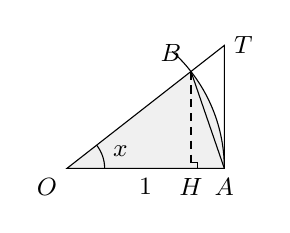
\begin{tikzpicture}[scale=2.0, font=\small]
\coordinate (O) at (0,0);
\coordinate (A) at (1,0);
\coordinate (B) at ({cos(38)},{sin(38)});
\coordinate (T) at (1,{tan(38)});
\coordinate (H) at ({cos(38)},0);
\fill[gray!12] (O)--(A) arc[start angle=0,end angle=38,radius=1]--cycle;
\draw (O)--(A)--(T)--cycle;
\draw (A)--(B);
\draw[densely dashed] (B)--(H);
\draw (H) ++(0,0.04)--++(0.04,0)--++(0,-0.04);
\draw (A) arc[start angle=0,end angle=48,radius=1];
\draw (0.24,0) arc[start angle=0,end angle=38,radius=0.24];
\node at (0.34,0.11) {$x$};
\node[below left] at (O) {$O$};
\node[below] at (A) {$A$};
\node[below] at (H) {$H$};
\node[above left] at (B) {$B$};
\node[right] at (T) {$T$};
\node[below] at (0.5,0) {$1$};
\end{tikzpicture}
\end{center}
作 $BH\perp OA$, 垂足为 $H$, 则 $BH=\sin x$. 比较三个图形的面积. $\triangle OAB$ 的底 $OA=1$, 高 $BH=\sin x$, 面积为 $\displaystyle\frac12\sin x$; 扇形 $OAB$ (图中阴影部分) 的半径为 $1$, 圆心角为 $x$, 面积为 $\displaystyle\frac12\cdot1^2\cdot x=\frac x2$; $\triangle OAT$ 的底 $OA=1$, 高 $AT=\tan x$, 面积为 $\displaystyle\frac12\tan x$.

三个图形依次包含. $\triangle OAB$ 中的每一点都在从 $O$ 到弦 $AB$ 上某一点的线段上. 弦 $AB$ 的两个端点在单位圆盘中, 而圆盘中两点的连线仍在圆盘中, 所以弦 $AB$ 上的点在圆盘中, 从 $O$ 到这些点的线段也在圆盘中; 这些线段又都在 $\angle AOB$ 内. 所以 $\triangle OAB$ 包含于扇形 $OAB$. 扇形中的每一点都在 $\angle AOB$ 内, 且与 $O$ 的距离不超过 $1$, 因而横坐标不超过 $1$; 而 $\triangle OAT$ 恰由 $\angle AOB$ 内横坐标不超过 $1$ 的点组成, 所以扇形包含于 $\triangle OAT$. 两次包含都少了一块面积为正的区域 (弦 $AB$ 与弧 $AB$ 之间的弓形, 以及弧 $AB$ 与线段 $BT$、$TA$ 之间的部分), 所以
\[
\frac12\sin x<\frac x2<\frac12\tan x,\qquad\text{即}\qquad\sin x<x<\tan x\quad\left(0<x<\frac\pi2\right).
\]
正弦是奇函数, 所以 $\displaystyle-\frac\pi2<x<0$ 时 $|\sin x|=\sin(-x)<-x=|x|$; 当 $\displaystyle|x|\ge\frac\pi2$ 时 $|\sin x|\le1<|x|$. 因此对一切 $x$ 都有 $|\sin x|\le|x|$.

由 $-|x|\le\sin x\le|x|$ 及两边夹定理, $\displaystyle\lim_{x\to0}\sin x=0$. 再由半角公式和复合函数的极限 (令 $\displaystyle u=\frac x2$),
\[
\lim_{x\to0}(1-\cos x)=\lim_{x\to0}2\sin^2\frac x2=2\left(\lim_{u\to0}\sin u\right)^2=0,
\]
所以 $\displaystyle\lim_{x\to0}\cos x=1$.
\end{cnproof}
任意一点 $c$ 处的极限可以由此得到. 令 $h=x-c$, 由和角公式及四则运算法则,
\[
\begin{aligned}
\lim_{x\to c}\sin x&=\lim_{h\to0}(\sin c\cos h+\cos c\sin h)=\sin c\cdot1+\cos c\cdot0=\sin c,\\
\lim_{x\to c}\cos x&=\lim_{h\to0}(\cos c\cos h-\sin c\sin h)=\cos c\cdot1-\sin c\cdot0=\cos c.
\end{aligned}
\]
\begin{theorem}[第一个重要极限]
$\displaystyle\lim_{x\to0}\frac{\sin x}x=1$.
\end{theorem}
由 $|\sin x|\le|x|$ 只知道比值的绝对值不超过 $1$, 还看不出它趋于 $1$, 需要一个同样趋于 $1$ 的下界. 上例中的另一半不等式 $x<\tan x$ 正好提供了它: 改写为 $\displaystyle\frac{\sin x}x>\cos x$.
\begin{cnproof}
当 $\displaystyle0<x<\frac\pi2$ 时, $\sin x>0$, $\cos x>0$. 由 $\sin x<x$ 得 $\displaystyle\frac{\sin x}x<1$; 由 $\displaystyle x<\frac{\sin x}{\cos x}$ 得 $\displaystyle\cos x<\frac{\sin x}x$. 所以
\[
\cos x<\frac{\sin x}x<1\qquad\left(0<x<\frac\pi2\right).
\]
由 $\displaystyle\lim_{x\to0}\cos x=1$ 及两边夹定理, 得右极限 $\displaystyle\lim_{x\to0^+}\frac{\sin x}x=1$. 由于 $\displaystyle\frac{\sin x}x$ 是偶函数, 左极限与右极限相等, 故 $\displaystyle\lim_{x\to0}\frac{\sin x}x=1$.
\end{cnproof}
\begin{example}
\textnormal{(教材例6.6)} 求 $\displaystyle\lim_{x\to0}\frac{1-\cos x}{2x^2}$.
\end{example}
\begin{cnsolution}
分子、分母都趋于零. 已知的极限是 $\displaystyle\frac{\sin u}u$ 型的, 而分子中只有余弦, 所以先用半角公式把 $1-\cos x$ 化为 $\displaystyle2\sin^2\frac x2$; 正弦的自变量是 $\displaystyle\frac x2$, 分母也要配成 $\displaystyle\left(\frac x2\right)^2$ 的倍数, 配出的常数要保留. 令 $\displaystyle u=\frac x2$, 由复合函数的极限及积的法则,
\[
\lim_{x\to0}\frac{1-\cos x}{2x^2}=\lim_{x\to0}\frac{2\sin^2\frac x2}{2x^2}=\lim_{x\to0}\frac14\left(\frac{\sin\frac x2}{\frac x2}\right)^2=\frac14\left(\lim_{u\to0}\frac{\sin u}u\right)^2=\frac14.
\]
\end{cnsolution}
由此得到以后常用的结果 $\displaystyle\lim_{x\to0}\frac{1-\cos x}{x^2}=\frac12$.
\begin{example}
\textnormal{(课堂例题: 第一个重要极限的基本变形)} 求
\[
\text{(1)}\ \lim_{x\to0}\frac x{\sin x};\qquad\text{(2)}\ \lim_{x\to\infty}x\sin\frac1x;\qquad\text{(3)}\ \lim_{x\to0}\frac{\tan x}x;\qquad\text{(4)}\ \lim_{x\to0}\frac{\sin2x}{\tan5x}.
\]
\end{example}
\par\indent\textbf{分析:} 使用第一个重要极限时, 正弦的自变量与分母必须是同一个趋于零的量. (1) 是基本极限的倒数, 用商的法则. (2) 中趋于零的量是 $\displaystyle\frac1x$, 所以令 $\displaystyle t=\frac1x$. (3) 把正切写成正弦与余弦之比. (4) 中有两个不同的角 $2x$ 与 $5x$, 要分别配成 $\displaystyle\frac{\sin2x}{2x}$ 与 $\displaystyle\frac{5x}{\sin5x}$, 配出的系数 $\displaystyle\frac{2x}{5x}=\frac25$ 保留下来.
\begin{cnsolution}
(1) 由商的法则,
\[
\lim_{x\to0}\frac x{\sin x}=\frac1{\displaystyle\lim_{x\to0}\frac{\sin x}x}=1.
\]

(2) 令 $\displaystyle t=\frac1x$, 当 $x\to\infty$ 时 $t\to0$, 且 $t\ne0$, 由复合函数的极限,
\[
\lim_{x\to\infty}x\sin\frac1x=\lim_{t\to0}\frac{\sin t}t=1.
\]

(3) 由 $\displaystyle\lim_{x\to0}\cos x=1\ne0$,
\[
\lim_{x\to0}\frac{\tan x}x=\lim_{x\to0}\left(\frac{\sin x}x\cdot\frac1{\cos x}\right)=1\cdot1=1.
\]

(4) 在 $0$ 的充分小的去心邻域内 $\sin5x\ne0$, $\cos5x\ne0$. 令 $u=2x$, $v=5x$, 由复合函数的极限及四则运算法则,
\[
\begin{aligned}
\lim_{x\to0}\frac{\sin2x}{\tan5x}
&=\lim_{x\to0}\left(\frac25\cdot\frac{\sin2x}{2x}\cdot\frac{5x}{\sin5x}\cdot\cos5x\right)\\
&=\frac25\cdot\lim_{u\to0}\frac{\sin u}u\cdot\frac1{\displaystyle\lim_{v\to0}\frac{\sin v}v}\cdot\lim_{x\to0}\cos5x=\frac25.
\end{aligned}
\]
\end{cnsolution}
\begin{example}
\textnormal{(课堂例题: 反三角函数的换元)} 求 $\displaystyle\lim_{x\to0}\frac{\arcsin x}x$ 及 $\displaystyle\lim_{x\to0}\frac{\arctan x}x$.
\end{example}
\par\indent\textbf{分析:} 已知的是三角函数的极限, 题中出现的却是反三角函数. 把反三角函数的值记为新的变量 $t$, 自变量就成为 $x=\sin t$ 或 $x=\tan t$, 式子回到上例的形式. 换元要用复合函数的极限, 须先验证 $x\to0$ 时 $t\to0$, 并且 $x\ne0$ 时 $t\ne0$. 前者由反三角函数的单调性得到: 要使 $|t|<\varepsilon$, 只需把 $x$ 限制在 $\sin\varepsilon$ 或 $\tan\varepsilon$ 以内, 但这需要 $\varepsilon$ 是一个合适的角, 所以先把 $\varepsilon$ 换成 $\displaystyle\eta=\min\left\{\varepsilon,\frac\pi4\right\}$.
\begin{cnsolution}
令 $t=\arcsin x$ ($|x|\le1$), 则 $x=\sin t$, $\displaystyle|t|\le\frac\pi2$. 先证 $x\to0$ 时 $t\to0$. 任给 $\varepsilon>0$, 令 $\displaystyle\eta=\min\left\{\varepsilon,\frac\pi4\right\}$, 取 $\delta=\sin\eta$. 当 $0<|x|<\delta$ 时, 由反正弦函数严格增加, $-\eta<\arcsin x<\eta$, 即 $|t|<\eta\le\varepsilon$. 又 $x\ne0$ 时 $t\ne0$. 由复合函数的极限及上例 (1),
\[
\lim_{x\to0}\frac{\arcsin x}x=\lim_{t\to0}\frac t{\sin t}=1.
\]
令 $t=\arctan x$, 则 $x=\tan t$. 对同样的 $\eta$, 当 $|x|<\tan\eta$ 时, 由反正切函数严格增加, $|t|<\eta\le\varepsilon$, 所以 $x\to0$ 时 $t\to0$; 又 $x\ne0$ 时 $t\ne0$. 由上例 (3),
\[
\lim_{x\to0}\frac{\arctan x}x=\lim_{t\to0}\frac t{\tan t}=\frac1{\displaystyle\lim_{t\to0}\frac{\tan t}t}=1.
\]
\end{cnsolution}
\begin{theorem}[第二个重要极限]
\[
\lim_{x\to\infty}\left(1+\frac1x\right)^x=e,\qquad\lim_{t\to0}(1+t)^{\frac1t}=e.
\]
\end{theorem}
\par\indent\textbf{分析:} 1.4 节已经证明 $\displaystyle\left(1+\frac1n\right)^n\to e$, 但那里 $n$ 是正整数, 现在 $x$ 取一切实数. 要把实数 $x$ 与整数联系起来, 可以用相邻的两个整数夹住它: 令 $n=[x]$, 则 $n\le x<n+1$. 于是底数 $\displaystyle1+\frac1x$ 夹在 $\displaystyle1+\frac1{n+1}$ 与 $\displaystyle1+\frac1n$ 之间. 指数为正时, 乘幂随底数增大而增大; 底数大于 $1$ 时, 乘幂随指数增大而增大. 所以 $\displaystyle\left(1+\frac1x\right)^x$ 夹在 $\displaystyle\left(1+\frac1{n+1}\right)^n$ 与 $\displaystyle\left(1+\frac1n\right)^{n+1}$ 之间. 两端稍加改写就是已知数列与一个趋于 $1$ 的因子之积或商, 都趋于 $e$.

$x\to-\infty$ 时底数小于 $1$, 上面的单调关系不能照搬. 令 $y=-x$, 则 $\displaystyle\left(1+\frac1x\right)^x=\left(\frac y{y-1}\right)^y$, 底数又成为 $\displaystyle1+\frac1{y-1}$, 可以化为已证的情形.
\begin{cnproof}
先设 $x\to+\infty$, 只需考虑 $x\ge1$. 令 $n=[x]$, 则 $n\ge1$, $n\le x<n+1$, 从而 $\displaystyle1<1+\frac1{n+1}<1+\frac1x\le1+\frac1n$. 这里的底数都大于 $1$, 指数都是正数, 由乘幂关于底数和指数的单调性,
\[
\left(1+\frac1{n+1}\right)^n\le\left(1+\frac1x\right)^x\le\left(1+\frac1n\right)^{n+1}.
\]
记
\[
b_n=\left(1+\frac1{n+1}\right)^n=\frac{\left(1+\frac1{n+1}\right)^{n+1}}{1+\frac1{n+1}},\qquad c_n=\left(1+\frac1n\right)^{n+1}=\left(1+\frac1n\right)^n\left(1+\frac1n\right).
\]
由 1.4 节 $e$ 的定义、去掉首项不改变极限以及四则运算法则, $b_n\to e$, $c_n\to e$. 任给 $\varepsilon>0$, 存在 $N$, 使 $n>N$ 时 $|b_n-e|<\varepsilon$, $|c_n-e|<\varepsilon$. 当 $x>N+1$ 时 $[x]>N$, 因而
\[
e-\varepsilon<b_{[x]}\le\left(1+\frac1x\right)^x\le c_{[x]}<e+\varepsilon.
\]
所以 $\displaystyle\lim_{x\to+\infty}\left(1+\frac1x\right)^x=e$.

再设 $x\to-\infty$. 令 $y=-x$, 当 $x<-2$ 时 $y>2$, 并且
\[
\left(1+\frac1x\right)^x=\left(1-\frac1y\right)^{-y}=\left(\frac y{y-1}\right)^y=\left(1+\frac1{y-1}\right)^{y-1}\left(1+\frac1{y-1}\right).
\]
记
\[
F(u)=\left(1+\frac1u\right)^u\left(1+\frac1u\right).
\]
由已证的情形、$\displaystyle\lim_{u\to+\infty}\left(1+\frac1u\right)=1$ 及积的法则, $\displaystyle\lim_{u\to+\infty}F(u)=e$. 任给 $\varepsilon>0$, 存在 $A>0$, 使 $u>A$ 时 $|F(u)-e|<\varepsilon$. 当 $x<-(A+2)$ 时, $u=y-1=-x-1>A+1$, 于是 $\displaystyle\left|\left(1+\frac1x\right)^x-e\right|=|F(u)-e|<\varepsilon$. 所以 $\displaystyle\lim_{x\to-\infty}\left(1+\frac1x\right)^x=e$. 两个方向的极限都是 $e$, 由 1.5 节定理1, 第一个等式成立.

最后证明第二个等式. 任给 $\varepsilon>0$, 由第一个等式, 存在 $A\ge1$, 使 $|x|>A$ 时 $\displaystyle\left|\left(1+\frac1x\right)^x-e\right|<\varepsilon$. 当 $\displaystyle0<|t|<\frac1A$ 时, $1+t>0$, 并且 $\displaystyle x=\frac1t$ 满足 $|x|>A$, 所以 $\bigl|(1+t)^{\frac1t}-e\bigr|<\varepsilon$.
\end{cnproof}
第二个重要极限中, 底数趋于 $1$ 而指数的绝对值无限增大. 这样的表达式俗称 $1^\infty$ 型, 它的极限由底数与 $1$ 的偏差和指数大小的相互关系决定, 不能分别对底数和指数取极限. 当底数和指数都有有限的极限且底数的极限为正时, 则可以分别取极限.
\begin{propositionsingle}[幂指函数的极限]
设 $\displaystyle\lim_{x\to a}u(x)=A$, $\displaystyle\lim_{x\to a}v(x)=B$, 且 $B>0$. 则 $\displaystyle\lim_{x\to a}v(x)^{u(x)}=B^A$.
\end{propositionsingle}
\begin{cnproof}
由保号性, $v(x)$ 在 $a$ 的某个去心邻域内为正, 可以写成 $v(x)^{u(x)}=e^{u(x)\ln v(x)}$. 由 1.5 节的习题1.5第3题, $\displaystyle\lim_{y\to B}\ln y=\ln B$; 外层函数 $\ln y$ 在 $B$ 处的值等于这个极限, 由复合函数极限后面的说明, $\ln v(x)\to\ln B$. 由积的法则, $u(x)\ln v(x)\to A\ln B$. 同理, 由 $\displaystyle\lim_{w\to w_0}e^w=e^{w_0}$ (教材例6.3), 得
\[
\lim_{x\to a}v(x)^{u(x)}=\lim_{x\to a}e^{u(x)\ln v(x)}=e^{A\ln B}=B^A.
\]
\end{cnproof}
命题对其他变化方式以及数列同样成立. 对 $1^\infty$ 型的极限 $\displaystyle\lim(1+u)^v$, 其中 $u\to0$, $|v|$ 无限增大, 可以借助第二个重要极限计算. 第二个重要极限提供的是整体 $(1+u)^{\frac1u}$, 为了用上它, 要把指数 $v$ 写成 $\displaystyle\frac1u$ 的倍数, 这个倍数只能是 $uv$:
\[
(1+u)^v=\left[(1+u)^{\frac1u}\right]^{uv}.
\]
方括号内的部分趋于 $e$. 若 $uv$ 趋于有限的数 $c$, 由上面的命题, 整个表达式趋于 $e^c$. 使用时要检验: 在所考察的范围内 $u\ne0$, 底数 $1+u>0$, 并且 $uv$ 有有限的极限.
\begin{example}
\textnormal{(教材例6.7)} 求 $\displaystyle\lim_{x\to\infty}\left(\frac{2x+1}{2x+3}\right)^x$.
\end{example}
\begin{cnsolution}
底数趋于 $1$, 指数的绝对值无限增大, 是 $1^\infty$ 型. 把底数写成 $1+t$, 其中 $\displaystyle t=\frac{2x+1}{2x+3}-1=-\frac2{2x+3}$. 当 $x\to\infty$ 时 $t\to0$; 当 $|x|>3$ 时 $t\ne0$, 且 $1+t>0$. 增量 $t$ 与指数的乘积为
\[
\lim_{x\to\infty}xt=\lim_{x\to\infty}\frac{-2x}{2x+3}=\lim_{x\to\infty}\frac{-2}{2+\frac3x}=-1.
\]
由第二个重要极限、复合函数的极限及幂指函数的极限,
\[
\lim_{x\to\infty}\left(\frac{2x+1}{2x+3}\right)^x=\lim_{x\to\infty}\left[(1+t)^{\frac1t}\right]^{xt}=e^{-1}.
\]
\end{cnsolution}
\begin{example}
\textnormal{(教材例6.8)} 设 $a>0$, $\mu\in\mathbb R$, 证明 $\displaystyle\lim_{x\to a}x^\mu=a^\mu$.
\end{example}
\begin{cnproof}
$\mu$ 是正整数时, 教材例5.2 已经用因式分解证明; 一般的实数 $\mu$ 没有这样的因式分解. 由对数的定义及运算法则, $x>0$ 时 $x^\mu=e^{\mu\ln x}$, 于是可以借助指数函数和对数函数的极限. 由 $a>0$, 在 $a$ 的邻域 $U(a,a)$ 内 $x>0$. 由习题1.5第3题及常数倍的法则, $\mu\ln x\to\mu\ln a$; 再由 $\displaystyle\lim_{w\to w_0}e^w=e^{w_0}$ 及复合函数极限后面的说明,
\[
\lim_{x\to a}x^\mu=\lim_{x\to a}e^{\mu\ln x}=e^{\mu\ln a}=a^\mu.
\]
\end{cnproof}
当 $\mu>0$ 时还有 $\displaystyle\lim_{x\to0^+}x^\mu=0$: 任给 $\varepsilon>0$, 当 $0<x<\varepsilon^{\frac1\mu}$ 时, 由幂函数 $x^\mu$ 在 $(0,+\infty)$ 上严格增加, $0<x^\mu<\varepsilon$.
\subsection{运算法则与重要极限的应用}
\begin{example}
\textnormal{(指定作业: 习题1.6第1题(4))} 求 $\displaystyle\lim_{x\to\infty}\frac{x^2-1}{2x^2-x-1}$.
\end{example}
\begin{cnsolution}
分子、分母都无限增大, 同除以最高次幂 $x^2$ 后各项都有有限的极限, 分母的极限不为零:
\[
\lim_{x\to\infty}\frac{x^2-1}{2x^2-x-1}=\lim_{x\to\infty}\frac{1-\frac1{x^2}}{2-\frac1x-\frac1{x^2}}=\frac{1-0}{2-0-0}=\frac12.
\]
\end{cnsolution}
\begin{example}
\textnormal{(指定作业: 习题1.6第1题(5))} 求 $\displaystyle\lim_{x\to1}\left(\frac1{1-x}-\frac3{1-x^3}\right)$.
\end{example}
\begin{cnsolution}
与教材例6.2 同型, 先通分. 由 $1-x^3=(1-x)(1+x+x^2)$, 通分后的分子 $x^2+x-2=(x-1)(x+2)$ 含有因子 $x-1$, 与分母中的 $1-x=-(x-1)$ 约去时出现一个负号. 在 $x\ne1$ 时,
\[
\begin{aligned}
\lim_{x\to1}\left(\frac1{1-x}-\frac3{1-x^3}\right)
&=\lim_{x\to1}\frac{(1+x+x^2)-3}{(1-x)(1+x+x^2)}=\lim_{x\to1}\frac{(x-1)(x+2)}{-(x-1)(1+x+x^2)}\\
&=\lim_{x\to1}\frac{-(x+2)}{1+x+x^2}=-1.
\end{aligned}
\]
\end{cnsolution}
\begin{example}
\textnormal{(指定作业: 习题1.6第1题(6))} 求 $\displaystyle\lim_{x\to4}\frac{\sqrt{2x+1}-3}{\sqrt{x-2}-\sqrt2}$.
\end{example}
\begin{cnsolution}
代入 $x=4$ 时分子、分母都为零. 根式之差中看不出因子 $x-4$, 分子、分母各乘以自己的共轭式后, 分子成为 $2x+1-9=2(x-4)$, 分母成为 $x-2-2=x-4$, 公因子就显露出来. 在 $4$ 的去心邻域 $\mathring U(4,2)$ 内,
\[
\begin{aligned}
\lim_{x\to4}\frac{\sqrt{2x+1}-3}{\sqrt{x-2}-\sqrt2}
&=\lim_{x\to4}\left(\frac{2(x-4)}{\sqrt{2x+1}+3}\cdot\frac{\sqrt{x-2}+\sqrt2}{x-4}\right)\\
&=\lim_{x\to4}\frac{2\left(\sqrt{x-2}+\sqrt2\right)}{\sqrt{2x+1}+3}=\frac{2\cdot2\sqrt2}{3+3}=\frac{2\sqrt2}3,
\end{aligned}
\]
其中根式的极限由本节例1 得到.
\end{cnsolution}
\begin{example}
\textnormal{(指定作业: 习题1.6第2题(4))} 求 $\displaystyle\lim_{x\to a}\frac{\sin x-\sin a}{x-a}$.
\end{example}
\begin{cnsolution}
分子是两个正弦之差, 分母是自变量之差, 两者都趋于零. 用和差化积把分子变成乘积 $\displaystyle2\cos\frac{x+a}2\sin\frac{x-a}2$, 其中正弦的自变量 $\displaystyle\frac{x-a}2$ 与分母只差一个常数倍. 令 $\displaystyle u=\frac{x-a}2$, 则 $x\to a$ 时 $u\to0$, $u\ne0$, 于是
\[
\lim_{x\to a}\frac{\sin x-\sin a}{x-a}=\lim_{x\to a}\left(\cos\frac{x+a}2\cdot\frac{\sin\frac{x-a}2}{\frac{x-a}2}\right)=\lim_{x\to a}\cos\frac{x+a}2\cdot\lim_{u\to0}\frac{\sin u}u=\cos a.
\]
余弦因子的极限由任意点处余弦的极限及复合函数极限后面的说明得到.
\end{cnsolution}
\begin{example}
\textnormal{(指定作业: 习题1.6第2题(6))} 求 $\displaystyle\lim_{x\to0}\frac{\tan x-\sin x}{\sin^3x}$.
\end{example}
\begin{cnsolution}
分子的两项都趋于零, 而且都与 $x$ 很接近, 相减以后剩下的量比 $x$ 小得多, 所以不能把分子的两项分开处理, 要先把差精确地化简. 把正切写成 $\displaystyle\frac{\sin x}{\cos x}$, 分子就成为 $\displaystyle\frac{\sin x(1-\cos x)}{\cos x}$; 约去 $\sin x$ 后, 剩下的 $\sin^2x$ 可以写成 $(1-\cos x)(1+\cos x)$, 再约去 $1-\cos x$. 在 $0$ 的充分小的去心邻域内 $\sin x\ne0$, $\cos x\ne0$, 由 $\sin^2x=(1-\cos x)(1+\cos x)$ 也有 $1-\cos x\ne0$, 于是
\[
\begin{aligned}
\lim_{x\to0}\frac{\tan x-\sin x}{\sin^3x}
&=\lim_{x\to0}\frac{\sin x(1-\cos x)}{\cos x\sin^3x}=\lim_{x\to0}\frac{1-\cos x}{\cos x(1-\cos x)(1+\cos x)}\\
&=\lim_{x\to0}\frac1{\cos x(1+\cos x)}=\frac1{1\cdot2}=\frac12.
\end{aligned}
\]
\end{cnsolution}
\begin{example}
\textnormal{(指定作业: 习题1.6第2题(8))} 求 $\displaystyle\lim_{x\to0}\frac{\sqrt{1-\cos x}}x$.
\end{example}
\begin{cnsolution}
由半角公式, $\displaystyle\sqrt{1-\cos x}=\sqrt2\left|\sin\frac x2\right|$, 开方后出现绝对值, 而分母 $x$ 带有符号, 所以分左、右两侧计算. 当 $0<x<\pi$ 时 $\displaystyle\sin\frac x2>0$, 令 $\displaystyle u=\frac x2$,
\[
\lim_{x\to0^+}\frac{\sqrt{1-\cos x}}x=\lim_{x\to0^+}\frac{\sqrt2\sin\frac x2}x=\frac{\sqrt2}2\lim_{u\to0^+}\frac{\sin u}u=\frac{\sqrt2}2.
\]
当 $-\pi<x<0$ 时 $\displaystyle\left|\sin\frac x2\right|=-\sin\frac x2$, 同理左极限为 $\displaystyle-\frac{\sqrt2}2$. 左、右极限不相等, 所求极限不存在.
\end{cnsolution}
\begin{example}
\textnormal{(指定作业: 习题1.6第2题(10))} 求 $\displaystyle\lim_{x\to0}(1-\tan x)^{\frac1{\sin x}}$.
\end{example}
\begin{cnsolution}
底数趋于 $1$, 指数的绝对值无限增大. 令 $t=-\tan x$, 则 $x\to0$ 时 $t\to0$; 在 $0$ 的充分小的去心邻域内 $t\ne0$, $1+t>0$. 增量与指数的乘积为
\[
\lim_{x\to0}\frac t{\sin x}=\lim_{x\to0}\frac{-\tan x}{\sin x}=\lim_{x\to0}\frac{-1}{\cos x}=-1,
\]
所以
\[
\lim_{x\to0}(1-\tan x)^{\frac1{\sin x}}=\lim_{x\to0}\left[(1+t)^{\frac1t}\right]^{\frac t{\sin x}}=e^{-1}.
\]
\end{cnsolution}
\begin{example}
\textnormal{(指定作业: 习题1.6第2题(11))} 求 $\displaystyle\lim_{x\to\infty}\left(\frac{2x-1}{2x+1}\right)^x$.
\end{example}
\begin{cnsolution}
与教材例6.7 同型. 令 $\displaystyle t=\frac{2x-1}{2x+1}-1=-\frac2{2x+1}$, 则 $x\to\infty$ 时 $t\to0$; 当 $|x|>2$ 时 $t\ne0$, $1+t>0$. 由
\[
\lim_{x\to\infty}xt=\lim_{x\to\infty}\frac{-2x}{2x+1}=\lim_{x\to\infty}\frac{-2}{2+\frac1x}=-1,
\]
得
\[
\lim_{x\to\infty}\left(\frac{2x-1}{2x+1}\right)^x=\lim_{x\to\infty}\left[(1+t)^{\frac1t}\right]^{xt}=e^{-1}.
\]
\end{cnsolution}
\begin{example}
\textnormal{(指定作业: 习题1.6第2题(13))} 对固定的实数 $x$, 求 $\displaystyle\lim_{n\to\infty}\left(1+\frac xn+\frac{x^2}{2n^2}\right)^{-n}$.
\end{example}
\begin{cnsolution}
这里变化的是 $n$, $x$ 是固定的参数. 底数趋于 $1$, 指数 $-n$ 的绝对值无限增大. 若 $x=0$, 各项都是 $1$, 极限为 $1$. 设 $x\ne0$, 令 $\displaystyle t_n=\frac xn+\frac{x^2}{2n^2}=\frac{2nx+x^2}{2n^2}$, 则 $t_n\to0$; 当 $\displaystyle n>\frac{|x|}2$ 时 $2nx+x^2\ne0$, 所以 $t_n\ne0$. 底数
\[
1+t_n=\frac12\left[\left(1+\frac xn\right)^2+1\right]>0.
\]
增量与指数的乘积的极限为
\[
\lim_{n\to\infty}(-nt_n)=\lim_{n\to\infty}\left(-x-\frac{x^2}{2n}\right)=-x,
\]
其中第二项 $\displaystyle\frac{x^2}{2n^2}$ 乘以 $n$ 后仍趋于零, 但在恒等变形完成之前不能把它删去. 由海涅定理, $\displaystyle(1+t_n)^{\frac1{t_n}}\to e$, 再由数列情形的幂指函数的极限,
\[
\lim_{n\to\infty}\left(1+\frac xn+\frac{x^2}{2n^2}\right)^{-n}=\lim_{n\to\infty}\left[(1+t_n)^{\frac1{t_n}}\right]^{-nt_n}=e^{-x}.
\]
$x=0$ 时结果 $1=e^0$ 也符合这个公式.
\end{cnsolution}
\begin{example}
\textnormal{(指定作业: 习题1.6第2题(14))} 求 $\displaystyle\lim_{x\to0}(\cos x)^{\frac1{x^2}}$.
\end{example}
\begin{cnsolution}
底数趋于 $1$, 指数无限增大. 令 $t=\cos x-1$, 则 $x\to0$ 时 $t\to0$; 在 $\displaystyle\mathring U\left(0,\frac\pi2\right)$ 内 $t\ne0$, $1+t=\cos x>0$. 由教材例6.6 后的结果,
\[
\lim_{x\to0}\frac t{x^2}=-\lim_{x\to0}\frac{1-\cos x}{x^2}=-\frac12,
\]
所以
\[
\lim_{x\to0}(\cos x)^{\frac1{x^2}}=\lim_{x\to0}\left[(1+t)^{\frac1t}\right]^{\frac t{x^2}}=e^{-\frac12}.
\]
\end{cnsolution}
\begin{example}
\textnormal{(指定作业: 习题1.6第6题)} 已知 $\displaystyle\lim_{x\to\infty}\left(\frac{x+a}{x-a}\right)^x=9$, 求常数 $a$.
\end{example}
\begin{cnsolution}
先把含参数 $a$ 的极限算出来, 再令它等于 $9$. 若 $a=0$, 表达式恒为 $1$, 极限为 $1\ne9$, 不合题意. 设 $a\ne0$, 令 $\displaystyle t=\frac{x+a}{x-a}-1=\frac{2a}{x-a}$, 则 $x\to\infty$ 时 $t\to0$; 当 $|x|>3|a|$ 时 $t\ne0$, 且 $|t|<1$, $1+t>0$. 由
\[
\lim_{x\to\infty}xt=\lim_{x\to\infty}\frac{2ax}{x-a}=\lim_{x\to\infty}\frac{2a}{1-\frac ax}=2a,
\]
得
\[
\lim_{x\to\infty}\left(\frac{x+a}{x-a}\right)^x=\lim_{x\to\infty}\left[(1+t)^{\frac1t}\right]^{xt}=e^{2a}.
\]
由 $e^{2a}=9$ 得 $2a=\ln9$, 即 $a=\ln3$.
\end{cnsolution}
\section{无穷小和无穷大}
前面关心的是变量趋于什么值, 本节比较变量趋于零或趋于无穷的快慢. 两个量同时趋于零时, 它们的差也趋于零, 差看不出谁快谁慢, 所以比较快慢要看它们的比值. 这种比较能找出表达式中起主要作用的部分, 从而简化极限的计算. 所有的比较都是在指定的极限过程中进行的.
\subsection{无穷小}
\begin{definition}
在某一极限过程中以 $0$ 为极限的函数, 称为这一过程中的\textbf{无穷小量}, 简称\textbf{无穷小}. 以 $0$ 为极限的数列也称为无穷小.
\end{definition}
无穷小是一个变量, 不是一个很小的数: 非零常数无论多么小都不是无穷小, 常数 $0$ 则是无穷小. 同一个函数在不同的过程中情况可能不同, 例如 $x$ 在 $x\to0$ 时是无穷小, 在 $x\to1$ 时不是. 所以说到无穷小, 必须指明极限过程.
\begin{example}
\textnormal{(教材例7.1)} 说明当 $x\to a$ 时 $(x-a)^2$ 与 $\sin(x-a)$ 是无穷小, 当 $x\to\infty$ 时 $\displaystyle\frac1x$、$\displaystyle\frac1{3x}$ 与 $\displaystyle\frac{x^2+x+1}{x^3+2}$ 是无穷小.
\end{example}
\begin{cnsolution}
只需验证各量在指定过程中的极限为零. 令 $h=x-a$, 当 $x\to a$ 时 $h\to0$, 所以 $(x-a)^2=h^2\to0$, $\sin(x-a)=\sin h\to0$. 当 $x\to\infty$ 时 $\displaystyle\frac1x\to0$, $\displaystyle\frac1{3x}=\frac13\cdot\frac1x\to0$. 最后一个量的分母次数高于分子, 同除以 $x^3$ 得
\[
\lim_{x\to\infty}\frac{x^2+x+1}{x^3+2}=\lim_{x\to\infty}\frac{\frac1x+\frac1{x^2}+\frac1{x^3}}{1+\frac2{x^3}}=\frac01=0.
\]
\end{cnsolution}
\begin{theoremsingle}
在同一极限过程中, $f\to L$ 的充分必要条件是 $f=L+\alpha$, 其中 $\alpha$ 是这一过程中的无穷小.
\end{theoremsingle}
\begin{cnproof}
若 $f\to L$, 令 $\alpha=f-L$, 由差的法则 $\alpha\to0$. 反过来, 若 $f=L+\alpha$, $\alpha\to0$, 由和的法则 $f\to L$.
\end{cnproof}
定理把“有极限”改写成“极限值加上一个无穷小”, 这样就可以进一步讨论误差 $\alpha$ 的大小.
\begin{proposition}
在同一极限过程中, 有限个无穷小之和是无穷小; 无穷小与局部有界的函数之积是无穷小. 特别地, 有限个无穷小之积是无穷小.
\end{proposition}
\begin{cnproof}
有限个无穷小之和由和的法则得到. 设 $\alpha\to0$, 而在所考察的范围内 $|\beta|\le M$, $M>0$. 任给 $\varepsilon>0$, 在相应的范围内 $\displaystyle|\alpha|<\frac\varepsilon M$, 于是 $|\alpha\beta|\le M|\alpha|<\varepsilon$, 所以 $\alpha\beta\to0$. 无穷小有极限, 由局部有界性, 它是局部有界的, 所以两个无穷小之积是无穷小.
\end{cnproof}
项数随过程变化时, 无穷小之和不一定是无穷小 (见 1.3 节运算法则后面的例子). 两个无穷小之商也没有确定的结论: 当 $x\to0$ 时, $\displaystyle\frac{x^2}x\to0$, $\displaystyle\frac{2x}x=2$, 而 $\displaystyle\frac x{x^2}=\frac1x$ 没有有限的极限. 商的这些不同情况, 就是后面比较无穷小的出发点.
\subsection{无穷大}
\begin{definition}
以 $x\to a$ 为例. 若对任意 $M>0$, 都存在 $\delta>0$, 使 $0<|x-a|<\delta$ 时恒有 $|f(x)|>M$, 则称当 $x\to a$ 时 $f(x)$ 为\textbf{无穷大量}, 简称\textbf{无穷大}, 记作 $\displaystyle\lim_{x\to a}f(x)=\infty$ 或 $f(x)\to\infty$ ($x\to a$). 若把条件 $|f(x)|>M$ 换成 $f(x)>M$ 或 $f(x)<-M$, 则分别称为\textbf{正无穷大}或\textbf{负无穷大}, 记作 $f(x)\to+\infty$ 或 $f(x)\to-\infty$. 其他极限过程以及数列的情形, 只需把去心邻域换成相应的范围.
\end{definition}
$\infty$ 不是实数. 写 $\displaystyle\lim_{x\to a}f(x)=\infty$ 时, 极限并不存在, 这个记号只描述 $|f(x)|$ 无限增大的情况. 定义要求相应范围内的\textbf{每一点}都满足 $|f(x)|>M$; 若只能找到一些点使 $|f(x)|$ 任意大, 只说明函数无界, 不能说明它是无穷大. 无穷大也不要求函数值在 $a$ 附近同号: 当 $x\to0$ 时 $\displaystyle\frac1x$ 是无穷大, 但它在左侧为负, 在右侧为正.
\begin{example}
\textnormal{(指定作业: 习题1.7第3题)} 函数 $f(x)=x\cos x$ 在 $\mathbb R$ 上是否有界? 当 $x\to\infty$ 时是否为无穷大?
\end{example}
\begin{cnsolution}
在余弦取 $1$ 的点处, $|f(x)|=|x|$ 可以任意大; 在余弦的零点处, $f(x)=0$. 这两类点在任意远处都有. 取 $x_n=2n\pi$, 则 $f(x_n)=2n\pi$, 可以超过任何正数, 所以 $f$ 在 $\mathbb R$ 上无界. 取 $\displaystyle y_n=n\pi+\frac\pi2$, 则 $f(y_n)=0$. 取 $M=1$, 对任意 $A>0$, 都存在 $n$ 使 $y_n>A$, 而 $|f(y_n)|=0<M$, 所以 $f$ 不满足无穷大的定义. 故 $f$ 无界, 但当 $x\to\infty$ 时不是无穷大.
\end{cnsolution}
\begin{example}
\textnormal{(教材例7.2)} 用定义证明 $\displaystyle\lim_{x\to1}\frac{x+2}{x^2-1}=\infty$.
\end{example}
\par\indent\textbf{分析:} 要对任意 $M>0$ 找出半径, 使去心邻域中 $\displaystyle\left|\frac{x+2}{x^2-1}\right|>M$. 分母趋于零, 分子趋于 $3$, 商的绝对值应当无限增大. 把分母分解为 $(x-1)(x+1)$, 原式的绝对值是
\[
\left|\frac{x+2}{x+1}\right|\cdot\frac1{|x-1|}.
\]
后一个因子在 $x\to1$ 时无限增大; 前一个因子趋于 $\displaystyle\frac32$, 给它一个正的下界, 就能由后一个因子的增大得到乘积的增大. 先把 $x$ 限制在 $\displaystyle|x-1|<\frac12$ 中, 这时 $x+1>0$, $\displaystyle\frac{x+2}{x+1}=1+\frac1{x+1}>1$, 原式的绝对值大于 $\displaystyle\frac1{|x-1|}$. 剩下只需 $\displaystyle\frac1{|x-1|}>M$, 即 $\displaystyle|x-1|<\frac1M$.
\begin{cnproof}
当 $\displaystyle0<|x-1|<\frac12$ 时, $\displaystyle\frac12<x<\frac32$, 所以
\[
\left|\frac{x+2}{x^2-1}\right|=\left(1+\frac1{x+1}\right)\frac1{|x-1|}>\frac1{|x-1|}.
\]
任给 $M>0$, 取 $\displaystyle\delta=\min\left\{\frac12,\frac1M\right\}$. 当 $0<|x-1|<\delta$ 时, $\displaystyle\left|\frac{x+2}{x^2-1}\right|>\frac1{|x-1|}>M$. 故 $\displaystyle\lim_{x\to1}\frac{x+2}{x^2-1}=\infty$.
\end{cnproof}
在上述范围内 $\displaystyle\frac{x+2}{x+1}>0$, 原式的符号与 $x-1$ 相同: $x\to1^-$ 时它是负无穷大, $x\to1^+$ 时它是正无穷大. 所以双侧只能写 $\infty$, 不能写 $+\infty$.
\begin{proposition}
在同一极限过程中: 若 $\alpha\to0$ 且 $\alpha$ 在所考察的范围内不为零, 则 $\displaystyle\frac1\alpha\to\infty$; 若 $f\to\infty$, 则 $\displaystyle\frac1f\to0$. 两个无穷大之积是无穷大; 无穷大与局部有界的函数之和是无穷大. 若 $g\to c\ne0$, $\alpha\to0$, 且 $\alpha$ 在所考察的范围内不为零, 则 $\displaystyle\frac g\alpha\to\infty$; 如果 $\alpha$ 在这个范围内与 $c$ 同号, 则 $\displaystyle\frac g\alpha\to+\infty$, 如果异号, 则 $\displaystyle\frac g\alpha\to-\infty$.
\end{proposition}
\begin{cnproof}
任给 $M>0$, 由 $\alpha\to0$, 在相应范围内 $\displaystyle0<|\alpha|<\frac1M$, 即 $\displaystyle\left|\frac1\alpha\right|>M$. 任给 $\varepsilon>0$, 由 $f\to\infty$, 在相应范围内 $\displaystyle|f|>\frac1\varepsilon$, 即 $\displaystyle\left|\frac1f\right|<\varepsilon$. 若 $f,g$ 都是无穷大, 任给 $M>0$, 在相应范围内两者的绝对值都大于 $\sqrt M$, 于是 $|fg|>M$. 若 $f\to\infty$ 而 $|g|\le C$, 任给 $M>0$, 在相应范围内 $|f|>M+C$, 由反三角不等式 $|f+g|\ge|f|-|g|>M$. 最后, 设 $g\to c\ne0$. 由保号性, 在相应范围内 $g$ 与 $c$ 同号且 $\displaystyle|g|>\frac{|c|}2$. 任给 $M>0$, 由 $\displaystyle\frac1\alpha\to\infty$, 在相应范围内 $\displaystyle\left|\frac1\alpha\right|>\frac{2M}{|c|}$, 于是 $\displaystyle\left|\frac g\alpha\right|>M$. $\displaystyle\frac g\alpha$ 的符号由 $g$ 与 $\alpha$ 的符号决定: $\alpha$ 与 $c$ 同号时它大于 $M$, 异号时它小于 $-M$.
\end{cnproof}
两个无穷大之和、无穷大与无穷小之积都没有确定的结论. 例如当 $x\to+\infty$ 时, $x$ 与 $-x$ 都是无穷大, 和为 $0$; 而 $\displaystyle x\cdot\frac1{x^2}\to0$, $\displaystyle x\cdot\frac1x=1$, $\displaystyle x\cdot\frac1{\sqrt x}=\sqrt x\to+\infty$. 这类情形要具体计算.
\subsection{无穷小的比较}
设 $x\to0$. $x$ 与 $x^2$ 都是无穷小, $x$ 与 $2x$ 也都是无穷小. 但 $x^2$ 比 $x$ 小得多: $x=0.01$ 时 $x^2=0.0001$, 只是 $x$ 的百分之一, 而且 $x$ 越小这个比例越小; $2x$ 则始终是 $x$ 的两倍. 要描述这种相对大小, 应以一个量为尺度, 看另一个量是它的多少倍, 也就是考察比值的极限.
\begin{definition}
设在同一极限过程中 $\alpha,\beta$ 都是无穷小, 且 $\beta$ 在所考察的范围内不为零.

\textup{(1)} 若 $\displaystyle\frac\alpha\beta\to0$, 则称 $\alpha$ 是比 $\beta$ \textbf{高阶的无穷小}, 记作 $\alpha=o(\beta)$.

\textup{(2)} 若 $\displaystyle\frac\alpha\beta\to k$, $k$ 是非零常数, 则称 $\alpha$ 与 $\beta$ 是\textbf{同阶无穷小}; 特别地, 若 $k=1$, 则称 $\alpha$ 与 $\beta$ 是\textbf{等价无穷小}, 记作 $\alpha\sim\beta$.

\textup{(3)} 若 $\displaystyle\left|\frac\alpha\beta\right|\to+\infty$, 则称 $\alpha$ 是比 $\beta$ \textbf{低阶的无穷小}.
\end{definition}
例如当 $x\to0$ 时 $x^2=o(x)$, $2x$ 与 $x$ 同阶但不等价, $\sin x\sim x$. 记号 $o(\beta)$ 表示某一个比 $\beta$ 高阶的无穷小, 它不是一个确定的函数, 所以 $o(\beta)-o(\beta)$ 未必等于 $0$; 另外约定 $o(1)$ 表示无穷小 (与常数 $1$ 之比趋于零的量). 比值的极限也可能不存在, 例如 $x\to0$ 时 $\displaystyle\frac{x\sin\frac1x}x=\sin\frac1x$, 这时两个量不能这样比较. 教材把同阶关系记作 $\alpha=O(\beta)$; 一般文献中的 $O$ 还可以表示比值有界这一较宽的关系, 本书作同阶判断时直接计算比值的极限.

比较的尺度通常取简单的无穷小, 例如 $x\to0$ 时取 $x$, $x\to\infty$ 时取 $\displaystyle\frac1x$.
\begin{definition}
设 $\beta$ 是同一过程中取作尺度的无穷小, $\mu>0$, 并且 $\beta^\mu$ 有意义 (例如 $\beta>0$, 或 $\mu$ 是正整数). 若 $\displaystyle\frac\alpha{\beta^\mu}\to k$, $k$ 是非零常数, 则称 $\alpha$ 是关于 $\beta$ 的 \textbf{$\mu$ 阶无穷小}, 并称 $k\beta^\mu$ 为 $\alpha$ 的\textbf{主部}.
\end{definition}
阶数越高, 趋于零越快. 主部同时反映大小和符号, 例如主部为 $-2x^3$ 表示 $\displaystyle\frac\alpha{x^3}\to-2$. 由定义, $k\beta^\mu$ 是 $\alpha$ 的主部当且仅当 $\alpha\sim k\beta^\mu$.
\begin{proposition}
在同一极限过程中, 设所涉及的无穷小在所考察的范围内都不为零.

\textup{(1)} $\alpha\sim\beta$ 的充分必要条件是 $\alpha=\beta+o(\beta)$.

\textup{(2)} 若 $\alpha\sim\beta$, 则 $\beta\sim\alpha$; 若 $\alpha\sim\beta$, $\beta\sim\gamma$, 则 $\alpha\sim\gamma$.

\textup{(3)} (等价替换) 设 $\alpha\sim\widetilde\alpha$, $f$ 是同一过程中的函数. 若 $\widetilde\alpha f$ 的极限存在或为 $\infty$, 则 $\alpha f$ 的极限也存在或为 $\infty$, 并且与前者相同; 若 $\displaystyle\frac f{\widetilde\alpha}$ 的极限存在或为 $\infty$, 则 $\displaystyle\frac f\alpha$ 也是如此. 因此乘积或商中的无穷小因子都可以换成与它等价的无穷小, 几个因子可以逐个替换.

\textup{(4)} 若 $\alpha\sim\widetilde\alpha$, $\beta\sim\widetilde\beta$, 且 $\displaystyle\frac{\widetilde\alpha}{\widetilde\beta}\to c$, $c\ne-1$, 则 $\alpha+\beta\sim\widetilde\alpha+\widetilde\beta$.
\end{proposition}
\begin{cnproof}
(1) 以 $\beta$ 为尺度衡量差 $\alpha-\beta$: $\displaystyle\frac{\alpha-\beta}\beta=\frac\alpha\beta-1$, 所以 $\displaystyle\frac\alpha\beta\to1$ 当且仅当 $\displaystyle\frac{\alpha-\beta}\beta\to0$, 即 $\alpha-\beta=o(\beta)$.

(2) 若 $\displaystyle\frac\alpha\beta\to1$, 由商的法则 $\displaystyle\frac\beta\alpha\to1$. 若还有 $\displaystyle\frac\beta\gamma\to1$, 则 $\displaystyle\frac\alpha\gamma=\frac\alpha\beta\cdot\frac\beta\gamma\to1$.

(3) 把替换前的表达式写成替换后的表达式乘以一个趋于 $1$ 的因子:
\[
\alpha f=\frac\alpha{\widetilde\alpha}\cdot\widetilde\alpha f,\qquad\frac f\alpha=\frac{\widetilde\alpha}\alpha\cdot\frac f{\widetilde\alpha}.
\]
若第二个因子有有限的极限 $c$, 由积的法则, 乘积也趋于 $c$. 若第二个因子是无穷大, 由保号性, 第一个因子在相应范围内大于 $\displaystyle\frac12$, 乘积的绝对值大于第二个因子的绝对值的一半, 所以乘积也是无穷大.

(4) 由 $c+1\ne0$ 及保号性, 在相应范围内 $\displaystyle\frac{\widetilde\alpha}{\widetilde\beta}+1\ne0$, 从而 $\widetilde\alpha+\widetilde\beta\ne0$. 于是
\[
\frac{\alpha+\beta}{\widetilde\alpha+\widetilde\beta}=\frac{\frac\alpha{\widetilde\alpha}\cdot\frac{\widetilde\alpha}{\widetilde\beta}+\frac\beta{\widetilde\beta}}{\frac{\widetilde\alpha}{\widetilde\beta}+1}\to\frac{1\cdot c+1}{c+1}=1.
\]
\end{cnproof}
(3) 说明, 乘积或商中的\textbf{因子}可以换成与它等价的量: 替换一个因子, 相当于乘上一个趋于 $1$ 的量, 不改变极限. 到目前为止, 当 $x\to0$ 时已知
\[
\sin x\sim x,\qquad\tan x\sim x,\qquad\arcsin x\sim x,\qquad\arctan x\sim x,\qquad1-\cos x\sim\frac{x^2}2,
\]
其中的 $x$ 换成任何一个在同一过程中趋于零 (且不为零) 的量 $u$ 也成立, 例如 $\sin(x^4)\sim x^4$. 1.8 节还将得到对数、指数和幂函数的几个等价关系.

和与差的情形不同. 由 (1), 替换 $\alpha\sim\widetilde\alpha$ 时丢掉的误差 $\alpha-\widetilde\alpha$ 只是比 $\widetilde\alpha$ 高阶, 不一定是零. 在乘积和商中, 这一相对误差不影响结果. 在和中, (4) 说明只要两个主部不相互抵消 ($c\ne-1$), 替换仍然可行. 但当 $c=-1$ 时, $\widetilde\alpha+\widetilde\beta$ 比 $\widetilde\alpha$ 本身小得多, 甚至可能等于零, 这时被丢掉的那些高阶误差可能与剩下的部分一样大, 甚至就是全部. 下面几个例子具体说明这一点.
\begin{example}
\textnormal{(教材例7.3)} 求 $\displaystyle\lim_{x\to0}\frac{x(\tan x-\sin x)}{\sin(x^4)}$.
\end{example}
\par\indent\textbf{分析:} 分子中 $\tan x$ 与 $\sin x$ 的主部都是 $x$, 相减时主部抵消, 不能分别替换. 要知道差有多大, 应先作精确的恒等变形. 把正切写成 $\displaystyle\frac{\sin x}{\cos x}$ 并通分:
\[
\tan x-\sin x=\frac{\sin x-\sin x\cos x}{\cos x}=\frac{\sin x(1-\cos x)}{\cos x}.
\]
差化成了乘积, 各因子的等价量都已知: $\sin x\sim x$, $\displaystyle1-\cos x\sim\frac{x^2}2$, $\cos x\to1$; 分母 $\sin(x^4)\sim x^4$. 这时可以逐个因子替换.
\begin{cnsolution}
在 $0$ 的充分小的去心邻域内 $\cos x\ne0$, $\sin(x^4)\ne0$. 由上面的恒等变形及等价替换,
\[
\lim_{x\to0}\frac{x(\tan x-\sin x)}{\sin(x^4)}=\lim_{x\to0}\frac{x\sin x(1-\cos x)}{\cos x\sin(x^4)}=\lim_{x\to0}\frac{x\cdot x\cdot\frac{x^2}2}{\cos x\cdot x^4}=\lim_{x\to0}\frac1{2\cos x}=\frac12.
\]
\end{cnsolution}
\begin{example}
\textnormal{(选自教材习题1.7第6题)} 求 $\displaystyle\lim_{x\to0}\frac{\tan x-\sin x}{x^3}$ 时, 为什么不能把 $\tan x$ 与 $\sin x$ 都换成 $x$?
\end{example}
\begin{cnsolution}
分别替换得到 $\displaystyle\frac{x-x}{x^3}=0$, 而由教材例7.3 中的恒等变形,
\[
\lim_{x\to0}\frac{\tan x-\sin x}{x^3}=\lim_{x\to0}\left(\frac{\sin x}x\cdot\frac{1-\cos x}{x^2}\cdot\frac1{\cos x}\right)=1\cdot\frac12\cdot1=\frac12,
\]
两者不同. 原因在于 $\tan x$ 与 $\sin x$ 是差中的项, 而且两项的主部 $x$ 相互抵消. 把它们写成
\[
\tan x=x+(\tan x-x),\qquad\sin x=x+(\sin x-x),
\]
替换就是丢掉误差 $\tan x-x$ 与 $\sin x-x$. 两个主部 $x$ 相减后完全抵消, 于是
\[
\tan x-\sin x=(\tan x-x)-(\sin x-x),
\]
原来的差全部由被丢掉的误差组成. 上面的计算表明 $\displaystyle\tan x-\sin x\sim\frac{x^3}2$, 所以这两个误差不可能都是比 $x^3$ 高阶的; 比值的极限 $\displaystyle\frac12$ 完全来自这两个误差, 而替换恰好把它们丢掉了. 用命题3(4) 来看, 这里 $\displaystyle\frac{\widetilde\alpha}{\widetilde\beta}=\frac x{-x}=-1$, 该命题的条件 $c\ne-1$ 不成立, 不能由它作替换; 上面的计算说明, 这时替换确实给出错误的结果.
\end{cnsolution}
\begin{example}
\textnormal{(指定作业: 习题1.7第7题(4))} 当 $x\to0$ 时, 求 $\tan x-\sin x$ 关于 $x$ 的阶与主部; 再求 $\displaystyle\lim_{x\to0}\frac{\tan x-\sin x}{x^2}$, 并与分母为 $x^3$ 的情形比较.
\end{example}
\begin{cnsolution}
由上例, $\displaystyle\lim_{x\to0}\frac{\tan x-\sin x}{x^3}=\frac12\ne0$, 所以 $\tan x-\sin x$ 是关于 $x$ 的三阶无穷小, 主部为 $\displaystyle\frac{x^3}2$. 分母换成 $x^2$ 时, 比值多出一个因子 $x$:
\[
\lim_{x\to0}\frac{\tan x-\sin x}{x^2}=\lim_{x\to0}\left(x\cdot\frac{\tan x-\sin x}{x^3}\right)=0\cdot\frac12=0.
\]
同一个三阶无穷小, 以低一阶的 $x^2$ 为尺度时比值趋于零, 以同阶的 $x^3$ 为尺度时比值趋于非零常数.
\end{cnsolution}
\begin{example}
\textnormal{(教材例7.4)} 当 $x\to0$ 时, $\sqrt{1+x^2}-\sqrt{1-x^2}$ 是关于 $x$ 的几阶无穷小?
\end{example}
\begin{cnsolution}
两个根式都趋于 $1$, 它们各自的极限反映不出差有多大, 先用共轭式把差精确地化开:
\[
\sqrt{1+x^2}-\sqrt{1-x^2}=\frac{(1+x^2)-(1-x^2)}{\sqrt{1+x^2}+\sqrt{1-x^2}}=\frac{2x^2}{\sqrt{1+x^2}+\sqrt{1-x^2}}.
\]
分母趋于 $2$, 所以应以 $x^2$ 为尺度. 当 $0<|x|<1$ 时,
\[
\lim_{x\to0}\frac{\sqrt{1+x^2}-\sqrt{1-x^2}}{x^2}=\lim_{x\to0}\frac2{\sqrt{1+x^2}+\sqrt{1-x^2}}=\frac2{1+1}=1.
\]
极限是非零常数, 故 $\sqrt{1+x^2}-\sqrt{1-x^2}$ 是二阶无穷小, 主部为 $x^2$.
\end{cnsolution}
判断阶数时, 比值的极限必须是非零常数. 若以 $x^\mu$ 为尺度时比值趋于零, 说明它的阶数高于 $\mu$; 若比值的绝对值无限增大, 说明阶数比 $\mu$ 低.
\begin{example}
\textnormal{(补充题型: 主部抵消与求参)} 求常数 $a$, 使 $\sqrt{1+x}-1-ax$ 在 $x\to0$ 时是关于 $x$ 的二阶无穷小, 并求它的主部.
\end{example}
\par\indent\textbf{分析:} 记 $R(x)=\sqrt{1+x}-1-ax$. 由有理化, $\displaystyle\sqrt{1+x}-1=\frac x{\sqrt{1+x}+1}\sim\frac x2$, 它是一阶的. 若 $\displaystyle a\ne\frac12$, $ax$ 抵消不掉这个一阶的主部, $R(x)$ 仍是一阶的; 要提高阶数, $ax$ 必须恰好抵消主部 $\displaystyle\frac x2$. 写成证明时, 用一个必要条件确定 $a$: 若 $\displaystyle\frac{R(x)}{x^2}\to k$, 则 $\displaystyle\frac{R(x)}x=x\cdot\frac{R(x)}{x^2}\to0$. 确定 $a$ 以后, 还要计算 $\displaystyle\frac{R(x)}{x^2}$ 的极限, 检验它不为零, 否则阶数比二阶更高.
\begin{cnsolution}
若 $R(x)$ 是二阶无穷小, 则 $\displaystyle\frac{R(x)}x\to0$. 而
\[
\lim_{x\to0}\frac{R(x)}x=\lim_{x\to0}\left(\frac1{\sqrt{1+x}+1}-a\right)=\frac12-a,
\]
所以必须 $\displaystyle a=\frac12$. 这时
\[
R(x)=\frac x{\sqrt{1+x}+1}-\frac x2=\frac{x\left(1-\sqrt{1+x}\right)}{2\left(\sqrt{1+x}+1\right)}=-\frac{x^2}{2\left(\sqrt{1+x}+1\right)^2},
\]
最后一步用了 $\displaystyle1-\sqrt{1+x}=-\frac x{1+\sqrt{1+x}}$. 于是
\[
\lim_{x\to0}\frac{R(x)}{x^2}=\lim_{x\to0}\frac{-1}{2\left(\sqrt{1+x}+1\right)^2}=-\frac18\ne0.
\]
故 $\displaystyle a=\frac12$, 此时 $R(x)$ 是二阶无穷小, 主部为 $\displaystyle-\frac{x^2}8$.
\end{cnsolution}
\begin{example}
\textnormal{(教材例7.5)} 当 $x\to+\infty$ 时, 求 $\displaystyle\frac1{x\sqrt{1+x^2}}$ 关于 $\displaystyle\frac1x$ 的主部, 并写成主部加高阶无穷小的形式.
\end{example}
\begin{cnsolution}
$x\to+\infty$ 时 $\sqrt{1+x^2}$ 与 $x$ 大小相当, 分母的大小与 $x^2$ 相当, 所以猜测主部为 $\displaystyle\frac1{x^2}$, 再用比值验证. 当 $x>0$ 时 $\sqrt{x^2}=x$, 于是
\[
\lim_{x\to+\infty}\frac{\frac1{x\sqrt{1+x^2}}}{\frac1{x^2}}=\lim_{x\to+\infty}\frac x{\sqrt{1+x^2}}=\lim_{x\to+\infty}\frac1{\sqrt{1+\frac1{x^2}}}=1.
\]
所以它是关于 $\displaystyle\frac1x$ 的二阶无穷小, 主部为 $\displaystyle\frac1{x^2}$, 并且
\[
\frac1{x\sqrt{1+x^2}}=\frac1{x^2}+o\!\left(\frac1{x^2}\right)\qquad(x\to+\infty).
\]
\end{cnsolution}
当 $x\to-\infty$ 时原式为负, $\sqrt{x^2}=-x$, 同样的比值趋于 $-1$, 主部是 $\displaystyle-\frac1{x^2}$. 所以写主部时必须注明过程.
\begin{example}
\textnormal{(指定作业: 习题1.7第5题(2)(4))} 证明
\[
\frac{x+2}{x^4+3}=o\!\left(\frac1{x^2}\right)\quad(x\to\infty),\qquad\sqrt{x+1}-\sqrt x=O\!\left(\frac1{\sqrt x}\right)\quad(x\to+\infty).
\]
第二式按教师更正取 $x\to+\infty$, $O$ 沿用教材的同阶约定.
\end{example}
\begin{cnproof}
两式都通过比值验证. 第一式的比值是多项式之商, 同除以最高次幂 $x^4$:
\[
\lim_{x\to\infty}\frac{\frac{x+2}{x^4+3}}{\frac1{x^2}}=\lim_{x\to\infty}\frac{x^3+2x^2}{x^4+3}=\lim_{x\to\infty}\frac{\frac1x+\frac2{x^2}}{1+\frac3{x^4}}=0,
\]
所以 $\displaystyle\frac{x+2}{x^4+3}=o\!\left(\frac1{x^2}\right)$. 第二式先把根式之差有理化:
\[
\lim_{x\to+\infty}\frac{\sqrt{x+1}-\sqrt x}{\frac1{\sqrt x}}=\lim_{x\to+\infty}\frac{\sqrt x}{\sqrt{x+1}+\sqrt x}=\lim_{x\to+\infty}\frac1{\sqrt{1+\frac1x}+1}=\frac12,
\]
比值趋于非零常数, 两者同阶, 并且 $\displaystyle\sqrt{x+1}-\sqrt x\sim\frac1{2\sqrt x}$.
\end{cnproof}
\begin{example}
\textnormal{(指定作业: 习题1.7第8题(4))} 求
\[
\lim_{x\to0^+}\frac{\sin(x^3)\tan x(1-\cos x)}{\sqrt{x+\sqrt[3]x}\,\sqrt[6]{x^5}\sin^5x}.
\]
\end{example}
\par\indent\textbf{分析:} 分子、分母都是若干因子的乘积, 可以逐个因子替换. 三角因子的等价量已知:
\[
\sin(x^3)\sim x^3,\qquad\tan x\sim x,\qquad1-\cos x\sim\frac{x^2}2,\qquad\sin^5x\sim x^5.
\]
因子 $\sqrt{x+\sqrt[3]x}$ 的根号内是一个和, 要先判断哪一项是主要的: $\displaystyle\frac x{\sqrt[3]x}=x^{\frac23}\to0$, 所以 $\sqrt[3]x$ 是主要的. 把它提出来, $x+\sqrt[3]x=x^{\frac13}\left(1+x^{\frac23}\right)$, 根式就等价于 $x^{\frac16}$.
\begin{cnsolution}
当 $x>0$ 时,
\[
\sqrt{x+\sqrt[3]x}=x^{\frac16}\sqrt{1+x^{\frac23}}\sim x^{\frac16},\qquad\sqrt[6]{x^5}=x^{\frac56},
\]
其中用到 $x\to0^+$ 时 $x^{\frac23}\to0$ (教材例6.8 后的说明), 从而 $\sqrt{1+x^{\frac23}}\to1$. 由等价替换,
\[
\lim_{x\to0^+}\frac{\sin(x^3)\tan x(1-\cos x)}{\sqrt{x+\sqrt[3]x}\,\sqrt[6]{x^5}\sin^5x}=\lim_{x\to0^+}\frac{x^3\cdot x\cdot\frac{x^2}2}{x^{\frac16}\cdot x^{\frac56}\cdot x^5}=\lim_{x\to0^+}\frac{x^6}{2x^6}=\frac12.
\]
\end{cnsolution}
对于有理函数, $x\to0$ 时分子、分母各取最低次项, $x\to\infty$ 时各取最高次项, 就是取主部后作等价替换.
\subsection{无穷大的比较}
无穷大同样用比值来比较.
\begin{definition}
设 $F,G$ 是同一过程中的无穷大. 若 $\displaystyle\frac FG$ 趋于非零常数, 则称 $F$ 与 $G$ 是\textbf{同阶无穷大}, 比值趋于 $1$ 时称它们\textbf{等价}; 若 $\displaystyle\frac FG\to0$, 则称 $F$ 是比 $G$ \textbf{低阶的无穷大}; 若 $\displaystyle\left|\frac FG\right|\to+\infty$, 则称 $F$ 是比 $G$ \textbf{高阶的无穷大}. 若 $\displaystyle\frac F{G^\mu}\to k$, 其中 $\mu>0$, $G^\mu$ 有意义, $k$ 是非零常数, 则称 $F$ 是关于 $G$ 的 \textbf{$\mu$ 阶无穷大}, $kG^\mu$ 称为 $F$ 的\textbf{主部}.
\end{definition}
主部为 $kG^\mu$ 时, $F=kG^\mu+o(G^\mu)$. 这里的 $o(G^\mu)$ 仍表示与 $G^\mu$ 之比趋于零的量, 它本身不一定趋于零.
\begin{example}
\textnormal{(教材例7.6)} 当 $x\to1$ 时, 求 $\displaystyle\frac1{\sin\pi x}$ 关于 $\displaystyle\frac1{x-1}$ 的阶与主部.
\end{example}
\par\indent\textbf{分析:} 按定义, 要计算比值 $\displaystyle\frac{x-1}{\sin\pi x}$ 的极限. 等价关系 $\sin u\sim u$ 要求 $u\to0$, 而这里 $\pi x\to\pi$, 不能直接使用. 令 $h=x-1$, 把趋近点移到零: $\sin\pi x=\sin(\pi+\pi h)=-\sin\pi h$, 其中 $\pi h\to0$. 诱导公式产生的负号决定了主部的符号.
\begin{cnsolution}
令 $h=x-1$, 当 $x\to1$ 时 $h\to0$, $h\ne0$, 且 $\sin\pi x=-\sin\pi h$. 由 $\sin\pi h\sim\pi h$,
\[
\lim_{x\to1}\frac{\frac1{\sin\pi x}}{\frac1{x-1}}=\lim_{x\to1}\frac{x-1}{\sin\pi x}=\lim_{h\to0}\frac h{-\sin\pi h}=\lim_{h\to0}\frac h{-\pi h}=-\frac1\pi.
\]
比值的极限是非零常数, 所以 $\displaystyle\frac1{\sin\pi x}$ 是关于 $\displaystyle\frac1{x-1}$ 的一阶无穷大, 主部为 $\displaystyle-\frac1{\pi(x-1)}$, 即
\[
\frac1{\sin\pi x}=-\frac1{\pi(x-1)}+o\!\left(\frac1{x-1}\right)\qquad(x\to1).
\]
\end{cnsolution}
\begin{example}
\textnormal{(教材例7.7)} 已知 $\displaystyle\lim_{x\to\infty}\left(\frac{x^2}{x+1}-ax-b\right)=0$, 求 $a,b$.
\end{example}
\par\indent\textbf{分析:} 题目要求 $\displaystyle\frac{x^2}{x+1}$ 与 $ax+b$ 之差趋于零. 只找出与 $\displaystyle\frac{x^2}{x+1}$ 等价的无穷大 $x$ 还不够: 等价只保证比值趋于 $1$, 差本身可以趋于非零常数, 甚至无界. 分子的次数比分母高一次, 用多项式除法可以把 $\displaystyle\frac{x^2}{x+1}$ 精确地写成一次式加真分式, 真分式趋于零, 一次式中的系数就决定了 $a,b$.
\begin{cnsolution}
由 $x^2=(x+1)(x-1)+1$ 得
\[
\frac{x^2}{x+1}-ax-b=(1-a)x-(1+b)+\frac1{x+1}.
\]
当 $x\to\infty$ 时 $\displaystyle\frac1{x+1}\to0$. 若 $a\ne1$, 则 $(1-a)x$ 是无穷大, 加上有界的其余两项仍是无穷大, 不可能趋于零, 所以 $a=1$. 这时差为 $\displaystyle-(1+b)+\frac1{x+1}$, 它趋于 $-(1+b)$, 由条件得 $b=-1$. 反过来, $a=1$, $b=-1$ 时差为 $\displaystyle\frac1{x+1}\to0$. 故 $a=1$, $b=-1$.
\end{cnsolution}
\section{连续函数}
函数在一点的极限只与该点附近的函数值有关, 与该点处的函数值无关. 如果进一步要求附近的函数值趋于该点处的函数值, 就得到连续的概念. 直观地看, 连续函数的图像在该点不断开. 本节先给出连续与间断的定义, 再证明连续性在四则运算、复合和取反函数时保持, 从而得到初等函数的连续性, 最后利用连续性得到对数、指数和幂函数的几个基本等价无穷小.
\subsection{连续与间断}
\begin{definition}
设 $f$ 在 $x_0$ 的某个邻域内有定义. 若对任意 $\varepsilon>0$, 都存在 $\delta>0$, 使当 $|x-x_0|<\delta$ 时恒有 $|f(x)-f(x_0)|<\varepsilon$, 则称 $f$ 在点 $x_0$ \textbf{连续}.
\end{definition}
与极限的定义相比, 这里有两处不同: 极限值换成了函数值 $f(x_0)$, 邻域也不再去心. 在 $x=x_0$ 处, $|f(x_0)-f(x_0)|=0<\varepsilon$ 自然成立, 所以 $f$ 在 $x_0$ 连续等价于三个条件同时成立: $f$ 在 $x_0$ 有定义, $\displaystyle\lim_{x\to x_0}f(x)$ 存在, 并且 $\displaystyle\lim_{x\to x_0}f(x)=f(x_0)$. 若记 $\Delta x=x-x_0$, $\Delta y=f(x_0+\Delta x)-f(x_0)$, 连续也可以说成: 当 $\Delta x\to0$ 时 $\Delta y\to0$, 即自变量的微小改变只引起函数值的微小改变.

若 $\displaystyle\lim_{x\to x_0^-}f(x)=f(x_0)$, 则称 $f$ 在 $x_0$ \textbf{左连续}; 若 $\displaystyle\lim_{x\to x_0^+}f(x)=f(x_0)$, 则称 $f$ 在 $x_0$ \textbf{右连续}. 由单侧极限与极限的关系, $f$ 在 $x_0$ 连续当且仅当它在 $x_0$ 既左连续又右连续. 设 $f$ 在数集 $E$ 上有定义. 若对每个 $x_0\in E$ 和任意 $\varepsilon>0$, 都存在 $\delta>0$, 使 $E$ 中满足 $|x-x_0|<\delta$ 的一切 $x$ 都有 $|f(x)-f(x_0)|<\varepsilon$, 则称 $f$ 在 $E$ 上\textbf{连续}. 当 $E$ 是区间时, 这就是说 $f$ 在 $E$ 的每个内点 (不是端点的点) 连续, 在 $E$ 所含的端点处单侧连续 (在左端点右连续, 在右端点左连续). 特别地, $f$ 在闭区间 $[a,b]$ 上连续, 是指它在 $(a,b)$ 内每一点连续, 在 $a$ 右连续, 在 $b$ 左连续; 这样的函数的全体记为 $C[a,b]$.
\begin{definition}
设 $f$ 在 $x_0$ 的某个去心邻域内有定义. 若 $f$ 在 $x_0$ 处没有定义, 或者有定义但不连续, 则称 $x_0$ 为 $f$ 的\textbf{间断点}. 若 $f$ 在 $x_0$ 处的左、右极限都存在, 则称 $x_0$ 为\textbf{第一类间断点}, 其中左、右极限相等时称为\textbf{可去间断点}, 不相等时称为\textbf{跳跃间断点}. 若左、右极限中至少有一个不存在, 则称 $x_0$ 为\textbf{第二类间断点}, 其中至少有一侧为无穷大时, 也称为\textbf{无穷间断点}.
\end{definition}
分类先看两侧的极限, 再看函数值. 在可去间断点处, 两侧的极限有共同的值 $L$, 只是 $f(x_0)$ 没有定义或 $f(x_0)\ne L$; 补充定义或改变定义, 令 $f(x_0)=L$, 函数在这一点就连续了, “可去”就是这个意思. 在跳跃间断点和第二类间断点处, 无论怎样规定 $f(x_0)$, 都不能使函数连续.
\begin{example}
\textnormal{(教材例8.1)} 讨论下列函数在 $x=0$ 处的连续性:
\[
f_1(x)=x^2,\quad f_2(x)=\begin{cases}|x|,&x\ne0,\\2,&x=0,\end{cases}\quad f_3(x)=\frac{\sin x}x\ (x\ne0),\quad f_4(x)=\begin{cases}e^{\frac1x},&x\ne0,\\1,&x=0.\end{cases}
\]
\end{example}
\begin{cnsolution}
对每个函数依次检查函数值是否有定义, 极限是否存在, 两者是否相等.

$f_1$: $\displaystyle\lim_{x\to0}x^2=0=f_1(0)$, 在 $0$ 连续.

$f_2$: $\displaystyle\lim_{x\to0}|x|=0$, 而 $f_2(0)=2$, 所以 $0$ 是可去间断点; 把 $f_2(0)$ 改为 $0$ 后连续.

$f_3$: 在 $0$ 处没有定义, 但 $\displaystyle\lim_{x\to0}\frac{\sin x}x=1$, 所以 $0$ 是可去间断点; 补充定义 $f_3(0)=1$ 后连续.

$f_4$: 与习题1.5第1题(5) 同样可证 $\displaystyle\lim_{x\to0^-}e^{\frac1x}=0$. 当 $x\to0^+$ 时, 任给 $M>1$, 只要 $\displaystyle0<x<\frac1{\ln M}$, 就有 $\displaystyle\frac1x>\ln M$, 从而 $e^{\frac1x}>M$, 所以 $e^{\frac1x}\to+\infty$. 右侧是无穷大, 所以 $0$ 是第二类间断点 (无穷间断点), 无论 $f_4(0)$ 取什么值都不连续.
\end{cnsolution}
又如取整函数 $[x]$: 在整数 $k$ 处, 左极限为 $k-1$, 右极限为 $k$, 所以 $k$ 是跳跃间断点; 在非整数点处 $[x]$ 是常数, 连续.
\begin{example}
\textnormal{(教材例8.2)} 设
\[
f(x)=\begin{cases}\frac{\sin x}x,&x<0,\\a,&x=0,\\x\sin\frac1x+b,&x>0.\end{cases}
\]
$a,b$ 满足什么条件时 $\displaystyle\lim_{x\to0}f(x)$ 存在? 满足什么条件时 $f$ 在 $0$ 连续?
\end{example}
\begin{cnsolution}
在分段点处要按两侧各自的表达式求左、右极限. 左极限是第一个重要极限: $\displaystyle\lim_{x\to0^-}\frac{\sin x}x=1$. 右侧的 $\displaystyle\sin\frac1x$ 没有极限, 但它有界, 由 $\displaystyle\left|x\sin\frac1x\right|\le|x|$ 及两边夹定理, $\displaystyle\lim_{x\to0^+}x\sin\frac1x=0$, 所以右极限为 $b$.

极限存在只要求左、右极限相等, 与函数值无关, 所以 $\displaystyle\lim_{x\to0}f(x)$ 存在当且仅当 $b=1$, 这时 $a$ 可以任意取值. 连续还要求函数值等于极限, 所以 $f$ 在 $0$ 连续当且仅当 $a=b=1$.
\end{cnsolution}
\subsection{连续函数的运算与初等函数的连续性}
\begin{theorem}
若 $f,g$ 都在 $x_0$ 连续, 则 $f\pm g$ 与 $fg$ 在 $x_0$ 连续; 若还有 $g(x_0)\ne0$, 则 $\displaystyle\frac fg$ 在 $x_0$ 连续. 若 $g$ 在 $x_0$ 连续, $f$ 在 $u_0=g(x_0)$ 连续, 并且复合函数 $f(g(x))$ 在 $x_0$ 的某个邻域内有定义, 则 $f(g(x))$ 在 $x_0$ 连续.
\end{theorem}
\begin{cnproof}
连续就是极限等于函数值, 所以前一部分由极限的四则运算法则直接得到. 例如
\[
\lim_{x\to x_0}f(x)g(x)=\lim_{x\to x_0}f(x)\cdot\lim_{x\to x_0}g(x)=f(x_0)g(x_0);
\]
商的情形用到 $g(x_0)\ne0$.

对复合函数, 由 $g$ 在 $x_0$ 连续, $\displaystyle\lim_{x\to x_0}g(x)=u_0$; 外层函数 $f$ 在 $u_0$ 有定义且 $\displaystyle\lim_{u\to u_0}f(u)=f(u_0)$. 由 1.6 节复合函数极限定理后面的说明, 这时不必要求 $g(x)\ne u_0$, 所以 $\displaystyle\lim_{x\to x_0}f(g(x))=f(u_0)=f(g(x_0))$.
\end{cnproof}
同样的道理给出计算极限时最常用的一条规则: 若 $\displaystyle\lim_{x\to a}g(x)=b$, 而 $f$ 在 $b$ 连续, 则
\[
\lim_{x\to a}f(g(x))=f(b)=f\left(\lim_{x\to a}g(x)\right),
\]
即对连续的外层函数, 极限号可以移到函数的内部. 这里不要求 $g$ 在 $a$ 处有定义, 也不要求 $g$ 在 $a$ 处连续.
\begin{example}
\textnormal{(教材例8.3)} 证明 $\sin x$ 在 $\mathbb R$ 上连续.
\end{example}
\begin{cnproof}
1.6 节已经由和角公式得到 $\displaystyle\lim_{x\to x_0}\sin x=\sin x_0$, 这就是连续性. 下面的证明还给出误差的明确估计. 任取 $x_0\in\mathbb R$. 两个正弦值本身都不一定小, 不便分开估计; 用和差化积把它们的差写成乘积, 其中一个因子 $\displaystyle\sin\frac{x-x_0}2$ 的自变量很小, 可以用 $|\sin t|\le|t|$, 另一个因子是余弦, 绝对值不超过 $1$:
\[
|\sin x-\sin x_0|=2\left|\cos\frac{x+x_0}2\right|\left|\sin\frac{x-x_0}2\right|\le2\cdot1\cdot\frac{|x-x_0|}2=|x-x_0|.
\]
任给 $\varepsilon>0$, 取 $\delta=\varepsilon$, 当 $|x-x_0|<\delta$ 时 $|\sin x-\sin x_0|<\varepsilon$. 故 $\sin x$ 在每一点连续. 同样,
\[
|\cos x-\cos x_0|=2\left|\sin\frac{x+x_0}2\right|\left|\sin\frac{x-x_0}2\right|\le|x-x_0|,
\]
所以 $\cos x$ 在 $\mathbb R$ 上连续.
\end{cnproof}
反三角函数是三角函数在单调区间上的反函数, 对数函数是指数函数的反函数. 下面的定理说明, 单调连续函数的反函数也连续.
\begin{theorem}[反函数的连续性]
设 $f$ 在区间 $I$ 上严格单调且连续, 则它的反函数 $f^{-1}$ 在 $f(I)$ 上与 $f$ 有相同的单调性, 并且在 $f(I)$ 上连续.
\end{theorem}
\par\indent\textbf{分析:} 设 $f$ 严格增加. 要证明 $f^{-1}$ 在 $y_0=f(x_0)$ 处连续, 就要对任意 $\varepsilon>0$ 找出 $\eta>0$, 使 $|y-y_0|<\eta$ 时 $|f^{-1}(y)-x_0|<\varepsilon$. 已知的条件都是关于 $f$ 的, 而要控制的是 $f^{-1}$ 的值, 方向正好相反. 单调性可以把大小关系在两边互相转换: 在 $x_0$ 两侧距离小于 $\varepsilon$ 的地方各取一点 $x_-<x_0<x_+$, 它们的像满足 $f(x_-)<y_0<f(x_+)$. 只要 $y$ 落在 $f(x_-)$ 与 $f(x_+)$ 之间, $f^{-1}(y)$ 就落在 $x_-$ 与 $x_+$ 之间, 与 $x_0$ 的距离小于 $\varepsilon$. 所以 $\eta$ 取 $y_0$ 到这两个像的距离中较小的一个.
\begin{cnproof}
设 $f$ 严格增加 (严格减少的情形把不等号反向). 严格单调的函数是单射, 所以反函数 $f^{-1}:f(I)\to I$ 存在. 若 $y_1<y_2$ 而 $f^{-1}(y_1)\ge f^{-1}(y_2)$, 则由 $f$ 严格增加得 $y_1\ge y_2$, 矛盾, 所以 $f^{-1}$ 也严格增加.

任取 $y_0\in f(I)$, 令 $x_0=f^{-1}(y_0)$, 并任给 $\varepsilon>0$. 先设 $x_0$ 不是 $I$ 的端点. 在 $I$ 中取 $x_-,x_+$, 使
\[
x_0-\varepsilon<x_-<x_0<x_+<x_0+\varepsilon,
\]
则 $f(x_-)<y_0<f(x_+)$. 取 $\eta=\min\{y_0-f(x_-),\,f(x_+)-y_0\}>0$. 若 $y\in f(I)$ 且 $|y-y_0|<\eta$, 则 $f(x_-)<y<f(x_+)$, 由 $f^{-1}$ 严格增加, $x_-<f^{-1}(y)<x_+$, 因而 $|f^{-1}(y)-x_0|<\varepsilon$.

若 $x_0$ 是 $I$ 的左端点, 则 $y_0$ 是 $f(I)$ 的最小值, 只需在 $x_0$ 右侧取 $x_+$, 令 $\eta=f(x_+)-y_0$, 同样的论证给出 $x_0\le f^{-1}(y)<x_+$. 右端点的情形类似. 所以 $f^{-1}$ 在 $f(I)$ 的每一点连续.
\end{cnproof}
证明中只用到了 $f$ 严格单调以及 $I$ 是区间. 1.9 节将由介值定理证明, 连续的条件保证 $f(I)$ 也是一个区间, 所以反函数是定义在区间上的连续函数.
\begin{theorem}[初等函数的连续性]
基本初等函数 (常数、幂函数、指数函数、对数函数、三角函数和反三角函数) 在各自的定义区间上连续. 由基本初等函数经有限次四则运算和复合得到的初等函数, 在其定义区间上连续.
\end{theorem}
\begin{cnproof}
常数函数在每一点连续. 指数函数 $a^x$ 的连续性见教材例6.3, 对数函数的连续性见习题1.5第3题 (一般的 $\displaystyle\log_ax=\frac{\ln x}{\ln a}$), 幂函数 $x^\mu$ 在 $x>0$ 处的连续性见教材例6.8; 当 $x^\mu$ 在负数处也有定义时 (例如 $\mu$ 为整数, 或 $\displaystyle\mu=\frac13$ 这样分母为奇数的有理数), 由 $x^\mu=\pm(-x)^\mu$ 及复合的连续性可得同样的结论, $\mu$ 为正整数时也可直接用教材例5.2; 当 $\mu>0$ 时, 由教材例6.8 后的说明, $\displaystyle\lim_{x\to0^+}x^\mu=0=0^\mu$, 即 $x^\mu$ 在 $0$ 处右连续 (在负数处也有定义时, 同理可得左连续). 正弦、余弦的连续性见上例, 正切、余切是它们的商, 在分母不为零处连续. 反正弦、反余弦和反正切分别是 $\sin x$ 在 $\displaystyle\left[-\frac\pi2,\frac\pi2\right]$、$\cos x$ 在 $[0,\pi]$、$\tan x$ 在 $\displaystyle\left(-\frac\pi2,\frac\pi2\right)$ 上的反函数, 由反函数的连续性, 它们在各自的定义区间上连续. 最后, 对基本初等函数反复应用四则运算与复合的连续性, 就得到关于初等函数的结论.
\end{cnproof}
这个定理把求极限的问题在许多情况下化为代入求值: 若 $f$ 是初等函数, $x_0$ 属于它的定义区间, 则 $\displaystyle\lim_{x\to x_0}f(x)=f(x_0)$. 使用时要确认 $x_0$ 在定义区间内; 分母为零、对负数开偶次方、对非正数取对数的点, 都不能直接代入.
\subsection{几个基本的等价无穷小}
有了连续性, 可以由第二个重要极限得到对数、指数和幂函数的几个基本极限.
\begin{example}
\textnormal{(教材例8.4)} 设 $a>0$, $a\ne1$, 求 $\displaystyle\lim_{x\to0}\frac{\log_a(1+x)}x$; 并求 $\displaystyle\lim_{x\to0}\frac{\ln(1+x)}{\sqrt{1+x}-1}$ (指定作业: 习题1.7第8题(2)).
\end{example}
\par\indent\textbf{分析:} 分子、分母都趋于零. 已知的极限中, 同时含有 $1+x$ 与 $\displaystyle\frac1x$ 的只有第二个重要极限 $(1+x)^{\frac1x}\to e$. 对数运算可以把系数 $\displaystyle\frac1x$ 移到真数的指数上: $\displaystyle\frac1x\log_a(1+x)=\log_a(1+x)^{\frac1x}$. 这样原式成为一个趋于 $e$ 的量的对数, 而对数函数在 $e$ 处连续, 极限号可以移到对数的内部. 第二个极限中, 分母的根式之差有理化以后成为 $\displaystyle\frac x{\sqrt{1+x}+1}$, 原式就化为第一个极限与一个连续因子的乘积.
\begin{cnsolution}
在 $0$ 的去心邻域 $\mathring U(0,1)$ 内 $1+x>0$. 由对数函数在 $e$ 处连续,
\[
\lim_{x\to0}\frac{\log_a(1+x)}x=\lim_{x\to0}\log_a(1+x)^{\frac1x}=\log_a\left(\lim_{x\to0}(1+x)^{\frac1x}\right)=\log_ae=\frac1{\ln a}.
\]
特别地, $\displaystyle\lim_{x\to0}\frac{\ln(1+x)}x=1$. 于是
\[
\lim_{x\to0}\frac{\ln(1+x)}{\sqrt{1+x}-1}=\lim_{x\to0}\frac{\ln(1+x)\left(\sqrt{1+x}+1\right)}x=\lim_{x\to0}\frac{\ln(1+x)}x\cdot\lim_{x\to0}\left(\sqrt{1+x}+1\right)=1\cdot2=2.
\]
\end{cnsolution}
\begin{example}
\textnormal{(教材例8.5)} 设 $a>0$, 求 $\displaystyle\lim_{x\to0}\frac{a^x-1}x$.
\end{example}
\par\indent\textbf{分析:} 上例处理的是对数的增量, 本题是指数的增量. 指数函数与对数函数互为反函数, 所以把指数的增量 $a^x-1$ 取作新的变量 $t$, 由 $x\ln a=\ln(1+t)$, 原式就化为上例中比值的倒数.
\begin{cnsolution}
若 $a=1$, 分子恒为 $0$, 极限为 $0=\ln1$. 设 $a\ne1$. 令 $t=a^x-1$, 由指数函数连续, $x\to0$ 时 $t\to0$; 由指数函数严格单调, $x\ne0$ 时 $t\ne0$. 由 $x\ln a=\ln(1+t)$,
\[
\lim_{x\to0}\frac{a^x-1}x=\lim_{t\to0}\frac{t\ln a}{\ln(1+t)}=\ln a\cdot\frac1{\displaystyle\lim_{t\to0}\frac{\ln(1+t)}t}=\ln a.
\]
\end{cnsolution}
\begin{example}
\textnormal{(教材例8.6)} 设 $\mu\in\mathbb R$, 求 $\displaystyle\lim_{x\to0}\frac{(1+x)^\mu-1}x$.
\end{example}
\par\indent\textbf{分析:} $\mu$ 为正整数时可以用二项式展开, 一般的实数 $\mu$ 不行. 由对数的定义及运算法则, $(1+x)^\mu=e^{\mu\ln(1+x)}$. 这样分子成为 $e^u-1$, 其中 $u=\mu\ln(1+x)\to0$. 前两例分别给出 $\displaystyle\frac{e^u-1}u\to1$ 与 $\displaystyle\frac{\ln(1+x)}x\to1$; 在分子、分母中同乘 $u$, 就能同时用上这两个结果:
\[
\frac{e^u-1}x=\frac{e^u-1}u\cdot\frac ux=\frac{e^u-1}u\cdot\mu\frac{\ln(1+x)}x.
\]
\begin{cnsolution}
若 $\mu=0$, 分子恒为 $0$, 极限为 $0$. 设 $\mu\ne0$. 在 $\mathring U(0,1)$ 内令 $u=\mu\ln(1+x)$, 由对数函数连续, $x\to0$ 时 $u\to0$; 由对数函数严格单调, $x\ne0$ 时 $u\ne0$. 于是
\[
\lim_{x\to0}\frac{(1+x)^\mu-1}x=\lim_{x\to0}\left(\frac{e^u-1}u\cdot\mu\cdot\frac{\ln(1+x)}x\right)=\lim_{u\to0}\frac{e^u-1}u\cdot\mu\cdot\lim_{x\to0}\frac{\ln(1+x)}x=\mu.
\]
\end{cnsolution}
以上三例给出当 $x\to0$ 时的等价无穷小
\[
\ln(1+x)\sim x,\qquad e^x-1\sim x,\qquad(1+x)^\mu-1\sim\mu x\quad(\mu\ne0),
\]
连同 1.7 节列出的 $\sin x\sim x$, $\tan x\sim x$, $\arcsin x\sim x$, $\arctan x\sim x$, $\displaystyle1-\cos x\sim\frac{x^2}2$, 构成等价替换中最常用的一组关系. 条件 $\mu\ne0$ 不能去掉, 因为 $\mu=0$ 时两边都恒为零. 其中的 $x$ 可以换成同一过程中任何趋于零且不为零的量, 例如 $x\to0$ 时 $\ln(1+x^2)\sim x^2$, $e^{\sin x}-1\sim\sin x\sim x$.
\begin{example}
\textnormal{(教材例8.7)} 已知当 $x\to0$ 时 $(1+ax^2)^{\frac13}-1$ 与 $\cos x-1$ 是等价无穷小, 求 $a$.
\end{example}
\begin{cnsolution}
等价要求两者之比趋于 $1$. 两个量都可以整体换成等价的幂函数, 比值就成为常数. 若 $a=0$, 第一个量恒为 $0$, 不是等价无穷小, 所以 $a\ne0$. 令 $u=ax^2$, 则 $x\to0$ 时 $u\to0$, $x\ne0$ 时 $u\ne0$, 由 $\displaystyle(1+u)^{\frac13}-1\sim\frac u3$ 得 $\displaystyle(1+ax^2)^{\frac13}-1\sim\frac a3x^2$; 又 $\displaystyle\cos x-1\sim-\frac{x^2}2$. 由等价替换,
\[
\lim_{x\to0}\frac{(1+ax^2)^{\frac13}-1}{\cos x-1}=\lim_{x\to0}\frac{\frac a3x^2}{-\frac{x^2}2}=-\frac{2a}3.
\]
令 $\displaystyle-\frac{2a}3=1$, 得 $\displaystyle a=-\frac32$. 此时当 $\displaystyle|x|<\sqrt{\frac23}$ 时 $1+ax^2>0$, 立方根 $(1+ax^2)^{\frac13}$ 按实数指数幂理解是有意义的.
\end{cnsolution}
\subsection{分段函数的连续性与间断点的判断}
分段函数在每一段内部通常由初等函数给出, 因而连续; 需要检查的是分段点. 在分段点处, 要按两侧各自的表达式分别求左、右极限, 再与函数值比较.
\begin{example}
\textnormal{(指定作业: 习题1.8第4题)} 设
\[
f(x)=\begin{cases}1+x^2,&x<0,\\a,&x=0,\\\frac{\sin bx}x,&x>0.\end{cases}
\]
$a,b$ 满足什么条件时 $\displaystyle\lim_{x\to0}f(x)$ 存在? 满足什么条件时 $f$ 在 $0$ 连续?
\end{example}
\begin{cnsolution}
左极限 $\displaystyle\lim_{x\to0^-}(1+x^2)=1$. 求右极限时, 正弦的自变量 $bx$ 与分母 $x$ 差一个因子 $b$, 要配成 $\displaystyle\frac{\sin bx}{bx}$, 这需要 $b\ne0$. 若 $b\ne0$, 令 $u=bx$,
\[
\lim_{x\to0^+}\frac{\sin bx}x=\lim_{x\to0^+}\left(b\cdot\frac{\sin bx}{bx}\right)=b\lim_{u\to0}\frac{\sin u}u=b;
\]
若 $b=0$, 右侧恒为 $0$, 右极限也等于 $b$. 所以 $\displaystyle\lim_{x\to0}f(x)$ 存在当且仅当 $b=1$, 这时 $a$ 任意; $f$ 在 $0$ 连续当且仅当 $a=b=1$.
\end{cnsolution}
\begin{example}
\textnormal{(课堂例题: 分段点处求连续参数)} 求参数, 使下列函数连续:
\[
\text{(1)}\ f(x)=\begin{cases}\frac{\sin(x^2-1)}{x-1},&x>1,\\a,&x\le1;\end{cases}\qquad\text{(2)}\ g(x)=\begin{cases}\frac{1-\cos\sqrt x}x,&x>0,\\ke^{x-1},&x\le0.\end{cases}
\]
\end{example}
\begin{cnsolution}
两个函数在各段内部都连续, 只需检查分段点. 在分段点处, 一侧的极限可以直接代入, 另一侧是分子、分母都趋于零的极限.

(1) $f(1)=a$, 左侧 $f$ 恒为 $a$, 左极限为 $a$. 右侧正弦的自变量是 $x^2-1$, 而分母是 $x-1$, 配成 $\displaystyle\frac{\sin(x^2-1)}{x^2-1}$ 后多出因子 $x+1$. 令 $u=x^2-1$, 当 $x\to1^+$ 时 $u\to0^+$, 于是
\[
\lim_{x\to1^+}\frac{\sin(x^2-1)}{x-1}=\lim_{x\to1^+}\left(\frac{\sin(x^2-1)}{x^2-1}\cdot(x+1)\right)=\lim_{u\to0^+}\frac{\sin u}u\cdot\lim_{x\to1^+}(x+1)=2.
\]
所以 $f$ 在 $1$ 连续当且仅当 $a=2$.

(2) $g(0)=ke^{-1}$, 左极限为 $\displaystyle\lim_{x\to0^-}ke^{x-1}=ke^{-1}$. 右侧令 $t=\sqrt x$, 则 $x=t^2$, 当 $x\to0^+$ 时 $t\to0^+$, 由 $\displaystyle1-\cos t\sim\frac{t^2}2$,
\[
\lim_{x\to0^+}\frac{1-\cos\sqrt x}x=\lim_{t\to0^+}\frac{1-\cos t}{t^2}=\frac12.
\]
所以 $g$ 在 $0$ 连续当且仅当 $\displaystyle ke^{-1}=\frac12$, 即 $\displaystyle k=\frac e2$.
\end{cnsolution}
\begin{example}
\textnormal{(课堂题型: 间断点分类)} 求下列函数的间断点, 并判断类型; 对可去间断点, 说明怎样补充或改变定义使函数连续:
\[
\begin{aligned}
&\text{(1)}\ \sin\frac1x;\qquad\text{(2)}\ \frac{\sin x}x;\qquad\text{(3)}\ p(x)=\begin{cases}\frac{\sin x}x,&x\ne0,\\0,&x=0;\end{cases}\qquad\text{(4)}\ q(x)=\begin{cases}\frac x{|x|},&x\ne0,\\0,&x=0;\end{cases}\\
&\text{(5)}\ \tan x;\qquad\text{(6)}\ \frac{x^2}{1-\cos x};\qquad\text{(7)}\ \frac1x\sin\frac1x.
\end{aligned}
\]
\end{example}
\begin{cnsolution}
初等函数在定义区间上连续, 所以间断点只可能是表达式没有定义的点或分段点. 找出这些点后, 先求左、右极限: 两侧极限都存在而且相等, 再看函数值; 两侧极限都存在但不相等, 是跳跃间断点; 至少有一侧的极限不存在, 是第二类间断点, 其中还要区分是否为无穷大.

(1) 只有 $x=0$ 没有定义. 教材例6.4 中的两列点 $x_n,y_n$ 都是正数, 由海涅定理 (单侧的形式), 右极限不存在, 同理左极限也不存在. 所以 $0$ 是第二类间断点, 函数值在 $-1$ 与 $1$ 之间振荡.

(2) 只有 $x=0$ 没有定义, 而 $\displaystyle\lim_{x\to0}\frac{\sin x}x=1$, 所以 $0$ 是可去间断点, 补充定义函数值为 $1$ 即连续.

(3) 函数值 $p(0)=0$, 而极限为 $1$, 所以 $0$ 是可去间断点, 把 $p(0)$ 改为 $1$ 即连续.

(4) 在 $0$ 处左极限为 $-1$, 右极限为 $1$, 所以 $0$ 是跳跃间断点, 改变 $q(0)$ 不能使它连续.

(5) $\tan x$ 在 $\displaystyle x_k=\frac\pi2+k\pi$ ($k\in\mathbb Z$) 处没有定义. 令 $h=x-x_k$, 则 $\displaystyle\tan x=\tan\left(h+\frac\pi2+k\pi\right)=-\frac{\cos h}{\sin h}$. 当 $h\to0^-$ 时, $-\cos h\to-1$, 而 $\sin h$ 是趋于零的负数, 与 $-1$ 同号, 由 1.7 节命题2, $\tan x\to+\infty$; 同理 $h\to0^+$ 时 $\tan x\to-\infty$. 每个 $x_k$ 都是无穷间断点.

(6) 分母 $1-\cos x=0$ 当且仅当 $x=2k\pi$ ($k\in\mathbb Z$). 当 $k=0$ 时, 由 $\displaystyle1-\cos x\sim\frac{x^2}2$ 得 $\displaystyle\lim_{x\to0}\frac{x^2}{1-\cos x}=2$, 所以 $0$ 是可去间断点, 补充定义函数值为 $2$ 即连续. 当 $k\ne0$ 时, 分子趋于 $(2k\pi)^2>0$, 分母是趋于零的正数, 由 1.7 节命题2, 函数是正无穷大, $2k\pi$ 是无穷间断点.

(7) 只有 $x=0$ 没有定义. 取 $\displaystyle x_n=\frac1{n\pi}$, 函数值为 $n\pi\sin n\pi=0$; 取 $\displaystyle y_n=\frac1{2n\pi+\frac\pi2}$, 函数值为 $\displaystyle2n\pi+\frac\pi2$, 可以超过任何正数. 两列点都从右侧趋于 $0$, 所以右极限不存在, 而且由于沿 $x_n$ 的函数值恒为 $0$, 右侧也不是无穷大. 这个函数是偶函数, 左侧的情况相同 (取 $-x_n$, $-y_n$). 所以 $0$ 是第二类间断点, 但不是无穷间断点. 这个例子说明, 函数在一点附近无界, 并不意味着它在这一点趋于无穷大.
\end{cnsolution}
\begin{example}
\textnormal{(指定作业: 习题1.8第5题)} 设 $\displaystyle f(x)=\frac{e^x-a}{x(x-1)}$. 已知 $x=1$ 是 $f$ 的可去间断点, 求 $a$, 并判断 $x=0$ 是哪一类间断点.
\end{example}
\par\indent\textbf{分析:} 可去间断要求 $\displaystyle\lim_{x\to1}f(x)$ 存在. 分母在 $x\to1$ 时趋于零, 若商有有限的极限, 那么分子 (分母与商之积) 必须趋于零, 由此得到 $a$ 应满足的必要条件; 然后还要验证, 对这个 $a$ 极限确实存在.
\begin{cnsolution}
若 $\displaystyle\lim_{x\to1}f(x)=L$ 存在, 则
\[
\lim_{x\to1}(e^x-a)=\lim_{x\to1}\bigl(f(x)\cdot x(x-1)\bigr)=L\cdot0=0,
\]
而 $\displaystyle\lim_{x\to1}(e^x-a)=e-a$, 所以 $a=e$. 反过来, 当 $a=e$ 时, 令 $h=x-1$, 由 $e^h-1\sim h$,
\[
\lim_{x\to1}f(x)=\lim_{h\to0}\frac{e(e^h-1)}{(1+h)h}=\lim_{h\to0}\frac{e\,h}{(1+h)h}=e,
\]
所以 $x=1$ 确实是可去间断点, 补充定义 $f(1)=e$ 即连续. 故 $a=e$.

在 $x=0$ 处, 分子趋于 $1-e<0$. 当 $x\to0^+$ 时分母 $x(x-1)$ 是趋于零的负数, 与分子的极限同号, 由 1.7 节命题2, $f(x)\to+\infty$; 当 $x\to0^-$ 时分母是趋于零的正数, $f(x)\to-\infty$. 所以 $x=0$ 是无穷间断点, 属于第二类.
\end{cnsolution}
\subsection{综合应用}
\begin{example}
\textnormal{(指定作业: 习题1.8第7题)} 设 $f$ 在 $0$ 的某个邻域内连续, 并且
\[
\lim_{x\to0}\left(1+x+\frac{f(x)}x\right)^{\frac1x}=e^3.
\]
求 $\displaystyle\lim_{x\to0}\left(1+\frac{f(x)}x\right)^{\frac1x}$.
\end{example}
\par\indent\textbf{分析:} 已知的和要求的都是 $1^\infty$ 型, 两个底数只差一个 $x$. 指数 $\displaystyle\frac1x$ 无界, 不能对底数和指数分别取极限. 取对数可以把乘幂化为商: 记 $\displaystyle B(x)=1+x+\frac{f(x)}x$, $C(x)=B(x)-x$, 已知条件给出 $\displaystyle\frac{\ln B(x)}x$ 的极限, 所求只需 $\displaystyle\frac{\ln C(x)}x$ 的极限. 两者之差是
\[
\frac{\ln B-\ln C}x=\frac1x\ln\frac BC=\frac1x\ln\left(1+\frac xC\right),
\]
这是 $\ln(1+u)$ 型, 其中 $\displaystyle u=\frac xC$. 要使 $u\to0$, 需要知道 $C$ 有非零的极限. 这可以从已知条件推出: $\ln B$ 等于 $x$ 乘以一个有极限的量, 所以趋于零, 从而 $B\to1$, $C\to1$. 这样做不需要预先知道 $\displaystyle\frac{f(x)}x$ 是否有极限.
\begin{cnsolution}
记 $\displaystyle B(x)=1+x+\frac{f(x)}x$, $C(x)=B(x)-x$. 由题设, 在 $0$ 的某个去心邻域内 $B(x)>0$. 由对数函数在 $e^3$ 处连续,
\[
\lim_{x\to0}\frac{\ln B(x)}x=\lim_{x\to0}\ln B(x)^{\frac1x}=\ln\left(\lim_{x\to0}B(x)^{\frac1x}\right)=\ln e^3=3.
\]
于是 $\displaystyle\ln B(x)=x\cdot\frac{\ln B(x)}x\to0$, 由指数函数连续, $B(x)=e^{\ln B(x)}\to1$, 从而 $C(x)=B(x)-x\to1$; 特别地, 在 $0$ 的某个去心邻域内 $C(x)>0$. 令 $\displaystyle u=\frac x{C(x)}$, 则 $x\to0$ 时 $u\to0$, 且 $x\ne0$ 时 $u\ne0$. 由 $B=C+x$,
\[
\lim_{x\to0}\frac{\ln B(x)-\ln C(x)}x=\lim_{x\to0}\frac{\ln\left(1+\frac x{C(x)}\right)}x=\lim_{x\to0}\left(\frac{\ln(1+u)}u\cdot\frac1{C(x)}\right)=1\cdot1=1.
\]
所以
\[
\lim_{x\to0}\frac{\ln C(x)}x=\lim_{x\to0}\frac{\ln B(x)}x-\lim_{x\to0}\frac{\ln B(x)-\ln C(x)}x=3-1=2.
\]
再由指数函数在 $2$ 处连续,
\[
\lim_{x\to0}\left(1+\frac{f(x)}x\right)^{\frac1x}=\lim_{x\to0}e^{\frac{\ln C(x)}x}=e^2.
\]
\end{cnsolution}
解答中没有用到 $f$ 的连续性. 题设还蕴含 $f(0)=0$: 由 $\displaystyle\frac{f(x)}x=C(x)-1\to0$ 得 $f(x)\to0$, 再由 $f$ 在 $0$ 连续知 $f(0)=0$.
\begin{example}
\textnormal{(指定作业: 习题1.8第11题(1)(4)(6))} 求
\[
\text{(1)}\ \lim_{x\to+\infty}x\bigl[\ln(x+1)-\ln x\bigr];\qquad\text{(4)}\ \lim_{x\to0}\frac{\sqrt{1-x\sin x}-1}{e^{x^2}-1};\qquad\text{(6)}\ \lim_{x\to0}\left(x+e^x\right)^{\frac1x}.
\]
\end{example}
\par\indent\textbf{分析:} (1) 两个对数都趋于无穷, 不能用差的法则. 用对数的运算把差合成一个对数 $\displaystyle\ln\frac{x+1}x=\ln\left(1+\frac1x\right)$, 真数偏离 $1$ 的量 $\displaystyle\frac1x$ 与前面的因子 $x$ 互为倒数, 正好是 $\displaystyle\frac{\ln(1+u)}u$ 的形式.

(4) 分子、分母都趋于零. 分子是根式减 $1$, 可以用 $\displaystyle(1+u)^{\frac12}-1\sim\frac u2$, 其中 $u=-x\sin x$; 也可以有理化. 分母 $e^{x^2}-1\sim x^2$. 替换以后都是因子的乘积.

(6) 底数 $x+e^x\to1$, 指数无界, 是 $1^\infty$ 型. 取对数后要求 $\displaystyle\frac{\ln(x+e^x)}x$ 的极限. 为了用 $\ln(1+u)\sim u$, 令 $u=x+e^x-1$, 再求 $\displaystyle\frac ux=1+\frac{e^x-1}x$ 的极限.
\begin{cnsolution}
(1) 当 $x>0$ 时, 令 $\displaystyle u=\frac1x$, 则 $x\to+\infty$ 时 $u\to0^+$, 于是
\[
\lim_{x\to+\infty}x\bigl[\ln(x+1)-\ln x\bigr]=\lim_{x\to+\infty}\frac{\ln\left(1+\frac1x\right)}{\frac1x}=\lim_{u\to0^+}\frac{\ln(1+u)}u=1.
\]

(4) 在 $0$ 的充分小的去心邻域内 $0<x\sin x<1$, $e^{x^2}-1\ne0$. 令 $u=-x\sin x$, 则 $u\to0$ 且 $u\ne0$, 由 $\displaystyle(1+u)^{\frac12}-1\sim\frac u2$, $e^{x^2}-1\sim x^2$ 及 $\sin x\sim x$,
\[
\lim_{x\to0}\frac{\sqrt{1-x\sin x}-1}{e^{x^2}-1}=\lim_{x\to0}\frac{-\frac12x\sin x}{x^2}=\lim_{x\to0}\frac{-\frac12x\cdot x}{x^2}=-\frac12.
\]

(6) 令 $u=x+e^x-1$, 由指数函数连续, $x\to0$ 时 $u\to0$. 又
\[
\lim_{x\to0}\frac ux=\lim_{x\to0}\left(1+\frac{e^x-1}x\right)=1+1=2,
\]
由保号性, 在 $0$ 的某个去心邻域内 $\displaystyle\frac ux>0$, 所以 $u\ne0$; 又由 $u\to0$, 在 $0$ 的某个去心邻域内 $|u|<1$, 底数 $1+u>0$. 于是
\[
\lim_{x\to0}\frac{\ln(x+e^x)}x=\lim_{x\to0}\left(\frac{\ln(1+u)}u\cdot\frac ux\right)=\lim_{u\to0}\frac{\ln(1+u)}u\cdot\lim_{x\to0}\frac ux=1\cdot2=2,
\]
再由指数函数连续,
\[
\lim_{x\to0}\left(x+e^x\right)^{\frac1x}=\lim_{x\to0}e^{\frac{\ln(x+e^x)}x}=e^2.
\]
\end{cnsolution}
\section{闭区间上连续函数的性质}
在一点连续只说明函数在这一点附近的情况. 本节讨论函数在整个闭区间上连续时具有的性质: 一致连续、有界、取得最大值和最小值、取得介于两个函数值之间的一切值. 前三条对开区间或无穷区间上的连续函数一般不成立, 介值性则对任何区间都成立 (见本节的推论). 这些性质的证明都要用到实数的完备性, 具体地说, 要用到 1.4 节的致密性定理或闭区间套定理. 以下闭区间 $[a,b]$ 都假定 $a<b$.

下面的证明多次用到连续函数与数列之间的一个关系. 1.6 节的海涅定理讨论的是去心邻域中的点列, 要求 $x_n\ne a$; 这里的点列可以取到极限点本身, 极限点也可以是区间的端点, 所以单独写出来.
\begin{propositionsingle}
设 $f\in C[a,b]$, $\{x_n\}$ 是 $[a,b]$ 中收敛于 $\xi$ 的数列, 则 $\xi\in[a,b]$, 并且 $f(x_n)\to f(\xi)$.
\end{propositionsingle}
\begin{cnproof}
由保序性, $\xi\in[a,b]$. 任给 $\varepsilon>0$, 由 $f$ 在 $\xi$ 处连续 ($\xi$ 是端点时为单侧连续), 存在 $\delta>0$, 使 $[a,b]$ 中满足 $|x-\xi|<\delta$ 的点都有 $|f(x)-f(\xi)|<\varepsilon$; 当 $x=\xi$ 时这个不等式自然成立. 当 $n$ 充分大时 $|x_n-\xi|<\delta$, 所以 $|f(x_n)-f(\xi)|<\varepsilon$.
\end{cnproof}
\subsection{一致连续性}
函数在区间上每一点连续, 是对每一点分别说的: 给定 $\varepsilon$ 后, 所找的 $\delta$ 可以随点 $x_0$ 改变. 例如 $\displaystyle f(x)=\frac1x$ 在 $(0,1)$ 内每一点连续. 取 $\varepsilon=1$, 点 $x_0$ 与 $\displaystyle\frac{x_0}2$ 相距 $\displaystyle\frac{x_0}2$, 函数值却相差 $\displaystyle\frac2{x_0}-\frac1{x_0}=\frac1{x_0}>1$, 所以在 $x_0$ 处适用的 $\delta$ 不能超过 $\displaystyle\frac{x_0}2$. $x_0$ 越接近 $0$, 适用的 $\delta$ 就必须越小, 没有一个对所有点都适用的 $\delta$. 若要求同一个 $\delta$ 对区间中的所有点都有效, 就得到更强的概念.
\begin{definitionsingle}
设 $f$ 定义在区间 $I$ 上. 若对任意 $\varepsilon>0$, 都存在 $\delta>0$, 使对任意 $x,y\in I$, 只要 $|x-y|<\delta$, 就有 $|f(x)-f(y)|<\varepsilon$, 则称 $f$ 在 $I$ 上\textbf{一致连续}.
\end{definitionsingle}
定义中 $\delta$ 只依赖于 $\varepsilon$ (以及函数和区间), 而不依赖于随后任取的 $x,y$; 这是与逐点连续的区别. 一致连续的函数在 $I$ 上每一点连续: 把 $y$ 固定为 $x_0$, 就得到连续的定义 ($x_0$ 是端点时得到单侧连续). 反过来不一定成立, 上面的 $\displaystyle\frac1x$ 就是例子.

否定一致连续, 就是要找一个固定的 $\varepsilon_0>0$, 使对每个 $\delta>0$, 都有距离小于 $\delta$ 的两点 $x,y\in I$, 而 $|f(x)-f(y)|\ge\varepsilon_0$. 通常构造两列点 $x_n,y_n\in I$, 使 $|x_n-y_n|\to0$, 而 $|f(x_n)-f(y_n)|$ 始终不小于某个正数.
\begin{example}
\textnormal{(教材例9.1)} 说明 $\displaystyle f(x)=\frac1x$ 与 $\displaystyle g(x)=\sin\frac1x$ 在 $(0,+\infty)$ 上连续, 但在任何区间 $(0,c)$ ($c>0$) 上都不一致连续.
\end{example}
\par\indent\textbf{分析:} 两个函数都是初等函数, 在 $(0,+\infty)$ 上连续. 要否定一致连续, 需要两列越来越靠近而函数值始终相差一个正数的点. 从函数值出发选点比较方便: 对 $\displaystyle\frac1x$, 让两列点的函数值是相邻的整数 $n+1$ 与 $n+2$, 相应的点是它们的倒数, 都趋于零, 距离也趋于零. 对 $\displaystyle\sin\frac1x$, 让函数值分别为 $1$ 与 $-1$, 相应的角可取 $\displaystyle2n\pi+\frac\pi2$ 与 $\displaystyle2n\pi+\frac{3\pi}2$, 点取这些角的倒数. 两列点都趋于零, 所以当 $n$ 充分大时都落在 $(0,c)$ 中.
\begin{cnsolution}
两个函数在 $(0,+\infty)$ 上连续, 这由初等函数的连续性得到.

对 $\displaystyle f(x)=\frac1x$, 取 $\displaystyle x_n=\frac1{n+1}$, $\displaystyle y_n=\frac1{n+2}$ ($n\in\mathbb N^+$), 则
\[
|x_n-y_n|=\frac1{n+1}-\frac1{n+2}=\frac1{(n+1)(n+2)}\to0,\qquad|f(x_n)-f(y_n)|=1.
\]
对 $\displaystyle g(x)=\sin\frac1x$, 取
\[
x_n=\frac1{2n\pi+\frac\pi2},\qquad y_n=\frac1{2n\pi+\frac{3\pi}2}\qquad(n\in\mathbb N^+),
\]
则 $0<y_n<x_n$, $|x_n-y_n|<x_n\to0$, 而 $g(x_n)=1$, $g(y_n)=-1$, $|g(x_n)-g(y_n)|=2$.

任给 $c>0$, 取 $\varepsilon_0=1$. 对任意 $\delta>0$, 上述两组点列都趋于 $0$, 并且每组中两点的距离趋于 $0$, 所以可以取充分大的 $n$, 使 $x_n,y_n\in(0,c)$ 且 $|x_n-y_n|<\delta$, 而相应的函数值之差不小于 $1=\varepsilon_0$. 所以两个函数在 $(0,c)$ 上都不一致连续.
\end{cnsolution}
$\displaystyle\frac1x$ 在 $(0,c)$ 上无界, 而 $\displaystyle\sin\frac1x$ 是有界的, 它不一致连续是因为越靠近 $0$ 振荡越快. 可见有界也不能保证一致连续.
\begin{example}
\textnormal{(教材例9.2)} 设 $0<a<1$, 证明 $\displaystyle f(x)=\frac1x$ 在 $[a,1]$ 上一致连续.
\end{example}
\par\indent\textbf{分析:} 按定义, 要估计任意两点处函数值之差. 通分得 $\displaystyle\left|\frac1x-\frac1y\right|=\frac{|x-y|}{xy}$, 其中 $|x-y|$ 是可以控制的距离, 因子 $\displaystyle\frac1{xy}$ 随点的位置变化. 在 $(0,c)$ 上这个因子可以任意大, 这是上例中 $\displaystyle\frac1x$ 不一致连续的原因; 现在 $x,y\ge a>0$, 它不超过 $\displaystyle\frac1{a^2}$, 于是函数值之差不超过 $\displaystyle\frac{|x-y|}{a^2}$, 由此可以找出与点的位置无关的 $\delta$.
\begin{cnproof}
对任意 $x,y\in[a,1]$, 有 $xy\ge a^2$, 所以
\[
\left|\frac1x-\frac1y\right|=\frac{|x-y|}{xy}\le\frac{|x-y|}{a^2}.
\]
任给 $\varepsilon>0$, 取 $\delta=a^2\varepsilon$. 对任意 $x,y\in[a,1]$, 只要 $|x-y|<\delta$, 就有 $\displaystyle\left|\frac1x-\frac1y\right|<\varepsilon$. 故 $f$ 在 $[a,1]$ 上一致连续.
\end{cnproof}
\begin{theorem}[一致连续定理]
闭区间 $[a,b]$ 上的连续函数在 $[a,b]$ 上一致连续.
\end{theorem}
\par\indent\textbf{分析:} 每一点的连续性各给出一个半径. 不能直接取所有这些半径的最小值: 点有无穷多个, 无穷多个正数不一定有最小值, 它们的下确界还可能是零. 换一个思路, 从一致连续的否定出发: 否定形式会给出具体的点列, 对点列可以使用 1.4 节关于数列的定理. 若不一致连续, 有一个固定的 $\varepsilon_0$, 对每个 $\displaystyle\delta=\frac1n$ 都有两点 $x_n,y_n$, 距离小于 $\displaystyle\frac1n$, 函数值之差却不小于 $\varepsilon_0$. 这些点的位置在变化, 不能对其中任何一点使用连续性. 致密性定理可以给出一个固定的点: $\{x_n\}$ 有收敛子列, 其极限 $\xi$ 在闭区间中, 而 $\{y_n\}$ 的相应子列也趋于 $\xi$. 在 $\xi$ 处使用连续性, 两列函数值都趋于 $f(\xi)$, 它们的差趋于零, 与差不小于 $\varepsilon_0$ 矛盾.
\begin{cnproof}
反设 $f$ 在 $[a,b]$ 上连续但不一致连续. 则存在 $\varepsilon_0>0$, 使对每个 $\delta>0$, 都有 $x,y\in[a,b]$ 满足 $|x-y|<\delta$ 而 $|f(x)-f(y)|\ge\varepsilon_0$. 对 $n=1,2,\ldots$, 取 $\displaystyle\delta=\frac1n$, 得到 $x_n,y_n\in[a,b]$, 满足
\[
|x_n-y_n|<\frac1n,\qquad|f(x_n)-f(y_n)|\ge\varepsilon_0.
\]
$\{x_n\}$ 有界, 由致密性定理, 它有收敛子列 $x_{n_k}\to\xi$, 由保序性 $\xi\in[a,b]$. 又
\[
|y_{n_k}-\xi|\le|y_{n_k}-x_{n_k}|+|x_{n_k}-\xi|<\frac1{n_k}+|x_{n_k}-\xi|,
\]
右端趋于零, 所以 $y_{n_k}\to\xi$. 由本节开头的命题, $f(x_{n_k})\to f(\xi)$, $f(y_{n_k})\to f(\xi)$, 从而 $f(x_{n_k})-f(y_{n_k})\to0$, 于是当 $k$ 充分大时 $|f(x_{n_k})-f(y_{n_k})|<\varepsilon_0$. 这与每一项都满足 $|f(x_{n_k})-f(y_{n_k})|\ge\varepsilon_0$ 矛盾. 故 $f$ 在 $[a,b]$ 上一致连续.
\end{cnproof}
区间是闭的, 保证了子列的极限 $\xi$ 仍在区间中, 是 $f$ 的连续点. 对于 $(0,c)$, 教材例9.1 中的点列趋于 $0$, 而 $0$ 不在区间中, 论证无法进行, 结论也确实不成立.
\subsection{有界性与最值}
\begin{theorem}[有界性定理]
若 $f\in C[a,b]$, 则 $f$ 在 $[a,b]$ 上有界, 即存在 $M>0$, 使每个 $x\in[a,b]$ 都满足 $|f(x)|\le M$.
\end{theorem}
\par\indent\textbf{分析:} 在每一点, 连续性只给出这一点附近的界, 无穷多个局部的界未必有共同的上界. 一致连续给出了一个对所有点都适用的半径: 对 $\varepsilon=1$ 取 $\delta$, 相距小于 $\delta$ 的两点的函数值相差小于 $1$. 于是把区间分成有限个长度小于 $\delta$ 的小段, 每一点的函数值都可以由某个分点的函数值加 $1$ 来控制, 而分点只有有限个.
\begin{cnproof}
由一致连续定理, 对 $\varepsilon=1$ 存在 $\delta>0$, 使 $x,y\in[a,b]$, $|x-y|<\delta$ 时 $|f(x)-f(y)|<1$. 由阿基米德性质, 取正整数 $m$ 使 $\displaystyle\frac{b-a}m<\delta$, 并令 $\displaystyle t_j=a+j\cdot\frac{b-a}m$ ($j=0,1,\ldots,m$). 每个 $x\in[a,b]$ 都落在某个 $[t_j,t_{j+1}]$ 中, 于是 $|x-t_j|<\delta$,
\[
|f(x)|\le|f(x)-f(t_j)|+|f(t_j)|<1+|f(t_j)|.
\]
令 $M=1+\max\{|f(t_0)|,|f(t_1)|,\ldots,|f(t_m)|\}$, 则每个 $x\in[a,b]$ 都满足 $|f(x)|\le M$.
\end{cnproof}
\begin{theorem}[最值定理]
若 $f\in C[a,b]$, 则存在 $x_*,x^*\in[a,b]$, 使每个 $x\in[a,b]$ 都满足 $f(x_*)\le f(x)\le f(x^*)$, 即 $f$ 在 $[a,b]$ 上取得最小值和最大值.
\end{theorem}
\par\indent\textbf{分析:} 先看最大值. 由有界性定理, 函数值的集合有上确界 $S$, 要找的是使 $f(x^*)=S$ 的点. 上确界不一定是函数值, 但由确界的刻画, 有函数值任意接近 $S$: 对每个 $n$, 有 $x_n$ 使 $\displaystyle S-\frac1n<f(x_n)\le S$. 这列点不一定收敛, 与上一小节一样, 用致密性定理取出收敛子列, 再在它的极限点处使用连续性.
\begin{cnproof}
由有界性定理, 非空数集 $\{f(x):x\in[a,b]\}$ 有上界, 设其上确界为 $S$. 由确界的刻画, 对每个正整数 $n$, 存在 $x_n\in[a,b]$, 使 $\displaystyle S-\frac1n<f(x_n)\le S$. 由致密性定理, $\{x_n\}$ 有收敛子列 $x_{n_k}\to x^*$, 且 $x^*\in[a,b]$. 由本节开头的命题, $f(x_{n_k})\to f(x^*)$; 又由 $\displaystyle S-\frac1{n_k}<f(x_{n_k})\le S$ 及两边夹定理, $f(x_{n_k})\to S$. 由极限的唯一性, $f(x^*)=S$, 所以每个 $x\in[a,b]$ 都满足 $f(x)\le f(x^*)$. 对 $-f$ 应用这一结论, 得到最小值点 $x_*$.
\end{cnproof}
最值定理比有界性定理更进一步: 函数值集合的上、下确界不仅存在, 而且在区间中被取到. 闭区间的条件不能去掉: $f(x)=x$ 在 $(0,1)$ 上连续且有界, 但既没有最大值也没有最小值; $\displaystyle\frac1x$ 在 $(0,1]$ 上连续, 却没有上界.
\begin{example}
\textnormal{(补充题型: 严格正函数的统一下界)} 设 $f\in C[a,b]$, 且每个 $x\in[a,b]$ 都有 $f(x)>0$. 证明存在 $m>0$, 使每个 $x\in[a,b]$ 都有 $f(x)\ge m$, 从而 $\displaystyle\frac1f$ 在 $[a,b]$ 上有界.
\end{example}
\par\indent\textbf{分析:} 每一点的函数值都是正数, 并不能直接得到一个共同的正下界: $f(x)=x$ 在 $(0,1)$ 上处处为正, 函数值的下确界却是 $0$. 在闭区间上, 最小值是某一点处的函数值, 因而是正数, 它就可以作为所求的下界.
\begin{cnproof}
由最值定理, 存在 $x_*\in[a,b]$ 使 $f(x_*)$ 是最小值. 令 $m=f(x_*)$, 它是一个函数值, 所以 $m>0$, 并且每个 $x\in[a,b]$ 都有 $f(x)\ge m$. 于是 $\displaystyle0<\frac1{f(x)}\le\frac1m$, 即 $\displaystyle\frac1f$ 在 $[a,b]$ 上有界.
\end{cnproof}
\subsection{零点定理与介值定理}
\begin{theorem}[零点定理]
若 $f\in C[a,b]$, 且 $f(a)$ 与 $f(b)$ 异号, 则存在 $\xi\in(a,b)$, 使 $f(\xi)=0$.
\end{theorem}
\par\indent\textbf{分析:} 零点的位置事先不知道, 而连续性只是每一点附近的性质, 不能直接指出零点. 可以逐步缩小零点所在的范围: 取区间的中点, 若函数在中点处为零, 零点已经找到; 否则中点处的函数值与某一个端点处同号, 舍去那一半, 剩下的半个区间两端仍然异号. 反复二分, 得到长度趋于零的闭区间套, 它们的公共点 $\xi$ 是可能的零点. 最后用连续性说明 $f(\xi)=0$: 设 $f(a)<0<f(b)$, 则各个左端点处的函数值都是负的, 右端点处都是正的, 两列端点都趋于 $\xi$, 所以 $f(\xi)$ 既不大于 $0$, 也不小于 $0$.
\begin{cnproof}
若 $f(a)>0>f(b)$, 对 $-f$ 讨论即可, 所以只需考虑 $f(a)<0<f(b)$ 的情形. 令 $[a_0,b_0]=[a,b]$. 设已得到 $[a_n,b_n]$, 满足 $f(a_n)<0<f(b_n)$. 取中点 $\displaystyle c_n=\frac{a_n+b_n}2$. 若 $f(c_n)=0$, 则 $\xi=c_n$ 就是所求的点; 由 $a\le a_n<c_n<b_n\le b$, 它属于 $(a,b)$. 若 $f(c_n)>0$, 令 $[a_{n+1},b_{n+1}]=[a_n,c_n]$; 若 $f(c_n)<0$, 令 $[a_{n+1},b_{n+1}]=[c_n,b_n]$. 两种情形都有 $f(a_{n+1})<0<f(b_{n+1})$.

若这一过程中始终没有遇到 $f(c_n)=0$, 就得到一串闭区间 $[a_n,b_n]$, 满足 $[a_{n+1},b_{n+1}]\subseteq[a_n,b_n]$,
\[
f(a_n)<0<f(b_n),\qquad b_n-a_n=\frac{b-a}{2^n}\to0.
\]
由闭区间套定理, 存在 $\xi\in[a,b]$, 使 $a_n\to\xi$, $b_n\to\xi$. 由本节开头的命题, $f(a_n)\to f(\xi)$, $f(b_n)\to f(\xi)$; 再由保序性, $f(\xi)\le0$ 且 $f(\xi)\ge0$, 所以 $f(\xi)=0$. 又 $f(a)\ne0$, $f(b)\ne0$, 故 $\xi\ne a,b$, 即 $\xi\in(a,b)$.
\end{cnproof}
二分法不仅证明了零点的存在, 还给出了一串逐步缩小的区间, 可以用来近似地求根. 区间中可能有多个零点, 二分法只找出其中一个.
\begin{theorem}[介值定理]
若 $f\in C[a,b]$, 且 $\mu$ 严格介于 $f(a)$ 与 $f(b)$ 之间, 则存在 $\xi\in(a,b)$, 使 $f(\xi)=\mu$.
\end{theorem}
\begin{cnproof}
要证明的等式 $f(\xi)=\mu$ 就是 $f(\xi)-\mu=0$, 所以考虑 $F(x)=f(x)-\mu$. $F\in C[a,b]$, 并且由 $\mu$ 严格介于 $f(a)$ 与 $f(b)$ 之间, $F(a)=f(a)-\mu$ 与 $F(b)=f(b)-\mu$ 异号. 由零点定理, 存在 $\xi\in(a,b)$ 使 $F(\xi)=0$, 即 $f(\xi)=\mu$.
\end{cnproof}
\begin{corollarysingle}
设 $f\in C[a,b]$, $m$ 与 $M$ 分别是 $f$ 在 $[a,b]$ 上的最小值与最大值, 则 $f$ 的值域是 $[m,M]$ ($m=M$ 时只含一点). 更一般地, 区间上的连续函数的值域是一个区间, 或者只含一点.
\end{corollarysingle}
\begin{cnproof}
设 $f(x_*)=m$, $f(x^*)=M$. 若 $m<\mu<M$, 则 $x_*\ne x^*$, 在以 $x_*,x^*$ 为端点的闭区间上应用介值定理, 得到使 $f(\xi)=\mu$ 的 $\xi$; 而 $m,M$ 本身是函数值. 所以值域是 $[m,M]$.

设 $f$ 在区间 $I$ 上连续. 若 $y_1<y_2$ 都是函数值, $y_1=f(x_1)$, $y_2=f(x_2)$, 则对 $y_1<\mu<y_2$, 在以 $x_1,x_2$ 为端点的闭区间 (它含于 $I$) 上应用介值定理, 知 $\mu$ 也是函数值. 所以值域中任意两数之间的数都属于值域. 若值域有上界, 记 $\beta$ 为它的上确界, 否则记 $\beta=+\infty$; 若值域有下界, 记 $\alpha$ 为它的下确界, 否则记 $\alpha=-\infty$. 对 $\alpha<\mu<\beta$, 由确界的刻画 (或值域无界), 值域中有 $y_1<\mu<y_2$, 于是 $\mu$ 属于值域. 另一方面, 每个函数值都不小于 $\alpha$, 也不大于 $\beta$. 所以值域由 $(\alpha,\beta)$ 以及 $\alpha,\beta$ 中属于值域的那些数组成: $\alpha<\beta$ 时它是以 $\alpha,\beta$ 为端点的区间, $\alpha=\beta$ 时它只含一点.
\end{cnproof}
若 $f$ 还严格单调, 则它是单射, 值域中的每个值只在一点取得. 推论的后半部分补全了 1.8 节反函数连续性定理后面的说明: 区间上严格单调的连续函数, 其反函数是定义在一个区间上的连续函数.
\begin{example}
\textnormal{(教材例9.3)} 证明方程 $x-\cos x=0$ 在 $\displaystyle\left(0,\frac\pi2\right)$ 内至少有一个实根.
\end{example}
\begin{cnproof}
方程的根就是函数 $F(x)=x-\cos x$ 的零点. $F$ 是初等函数, 在 $\displaystyle\left[0,\frac\pi2\right]$ 上连续. 在两个端点处, $x$ 与 $\cos x$ 分别有一个为零, 符号容易判断:
\[
F(0)=0-1=-1<0,\qquad F\!\left(\frac\pi2\right)=\frac\pi2-0>0.
\]
由零点定理, 存在 $\displaystyle\xi\in\left(0,\frac\pi2\right)$, 使 $F(\xi)=0$, 即 $\xi-\cos\xi=0$.
\end{cnproof}
\begin{example}
\textnormal{(指定作业: 习题1.9第1题)} 证明方程 $x\cdot2^x=1$ 至少有一个小于 $1$ 的正根.
\end{example}
\begin{cnproof}
小于 $1$ 的正根就是 $(0,1)$ 中的根. 令 $F(x)=x\cdot2^x-1$, 由初等函数的连续性, $F\in C[0,1]$. 又 $F(0)=-1<0$, $F(1)=2-1=1>0$, 由零点定理, 存在 $\xi\in(0,1)$, 使 $F(\xi)=0$, 即 $\xi\cdot2^\xi=1$.
\end{cnproof}
零点定理只说明根的存在. 若还要说明根是唯一的, 需要另外的论证, 例如说明函数严格单调.
\begin{example}
\textnormal{(补充应用)} 证明方程 $x^3+x-1=0$ 在 $(0,1)$ 内恰有一个实根.
\end{example}
\begin{cnproof}
令 $F(x)=x^3+x-1$, 则 $F\in C[0,1]$, $F(0)=-1<0$, $F(1)=1>0$, 由零点定理, $F$ 在 $(0,1)$ 内至少有一个零点. 再说明零点只有一个. 这里还没有引入导数, 可以直接比较函数值: 若 $0\le x<y\le1$, 则
\[
F(y)-F(x)=(y^3-x^3)+(y-x)=(y-x)(y^2+xy+x^2+1)>0,
\]
所以 $F$ 在 $[0,1]$ 上严格增加, 不可能在两个不同的点都取值 $0$. 故方程在 $(0,1)$ 内恰有一个实根.
\end{cnproof}
\begin{example}
\textnormal{(指定作业: 习题1.9第11题)} 设 $n$ 为奇数, $a_0,a_1,\ldots,a_n\in\mathbb R$, $a_n\ne0$. 证明方程
\[
a_nx^n+a_{n-1}x^{n-1}+\cdots+a_1x+a_0=0
\]
至少有一个实根.
\end{example}
\par\indent\textbf{分析:} 题目没有给出区间, 需要先找出两个函数值异号的点. 记方程左边为 $P(x)$. $|x|$ 很大时, 最高次项 $a_nx^n$ 起主要作用, 而 $n$ 是奇数, $x^n$ 在正、负两侧符号相反, 所以 $P(x)$ 在两侧应当异号. 要把“起主要作用”写成严格的推理, 可以考虑 $\displaystyle\frac{P(x)}{x^n}$: 它趋于 $a_n\ne0$, 由保号性, $|x|$ 充分大时它与 $a_n$ 同号, 再乘以 $x^n$, 就得到 $P(x)$ 在两侧的符号.
\begin{cnproof}
若 $n=1$, $\displaystyle x=-\frac{a_0}{a_1}$ 就是实根. 设 $n\ge3$. 对 $x\ne0$,
\[
\lim_{x\to\infty}\frac{P(x)}{x^n}=\lim_{x\to\infty}\left(a_n+\frac{a_{n-1}}x+\cdots+\frac{a_1}{x^{n-1}}+\frac{a_0}{x^n}\right)=a_n\ne0,
\]
其中 $x\to\infty$ 包括正、负两个方向, 因为每一项 $\displaystyle\frac{a_j}{x^{n-j}}$ ($j<n$) 在两个方向都趋于零. 由保号性, 存在 $A>0$, 使 $|x|>A$ 时 $\displaystyle\frac{P(x)}{x^n}$ 与 $a_n$ 同号. 取 $R>A$. 由于 $R^n>0$, $(-R)^n<0$, 所以 $\displaystyle P(R)=R^n\cdot\frac{P(R)}{R^n}$ 与 $a_n$ 同号, $\displaystyle P(-R)=(-R)^n\cdot\frac{P(-R)}{(-R)^n}$ 与 $a_n$ 异号, 从而 $P(-R)$ 与 $P(R)$ 异号. $P$ 在 $[-R,R]$ 上连续, 由零点定理, 存在 $\xi\in(-R,R)$, 使 $P(\xi)=0$.
\end{cnproof}
偶数次多项式没有这一结论, 例如 $x^2+1=0$ 没有实根. 对偶数次多项式, $|x|$ 充分大时 $P(x)$ 与 $P(-x)$ 同号, 上面的论证不能进行; 而 $x^2+1$ 的值都是正数.
\begin{example}
\textnormal{(补充应用)} 设 $f:[a,b]\to[a,b]$ 连续. 证明存在 $\xi\in[a,b]$, 使 $f(\xi)=\xi$.
\end{example}
\begin{cnproof}
要证明的等式 $f(\xi)=\xi$ 就是 $f(\xi)-\xi=0$, 所以考虑 $F(x)=f(x)-x$, 它在 $[a,b]$ 上连续. 端点处的符号由值域的条件给出: $f(a)\in[a,b]$, 所以 $F(a)=f(a)-a\ge0$; 同理 $F(b)=f(b)-b\le0$. 若 $F(a)=0$ 或 $F(b)=0$, 相应的端点就是所求的 $\xi$. 否则 $F(a)>0>F(b)$, 由零点定理, 存在 $\xi\in(a,b)$ 使 $F(\xi)=0$. 两种情形都有 $f(\xi)=\xi$.
\end{cnproof}
\begin{example}
\textnormal{(指定作业: 习题1.9第3题)} 设 $f\in C[a,b]$, $a<x_1<x_2<\cdots<x_n<b$. 证明存在 $\xi\in[x_1,x_n]$, 使
\[
f(\xi)=\frac{f(x_1)+f(x_2)+\cdots+f(x_n)}n.
\]
\end{example}
\par\indent\textbf{分析:} 要证明某个函数值等于给定的数 $A$ (这里是平均值), 应当用介值定理, 为此要先找两个函数值, 使 $A$ 介于它们之间. $A$ 不一定介于 $f(x_1)$ 与 $f(x_n)$ 之间, 因为这 $n$ 个函数值不一定按大小排列. 但 $n$ 个数的平均值一定介于其中最小者与最大者之间, 所以在这两个函数值对应的点之间使用介值定理, 这个区间含于 $[x_1,x_n]$.
\begin{cnproof}
记 $\displaystyle A=\frac{f(x_1)+\cdots+f(x_n)}n$. 在 $f(x_1),\ldots,f(x_n)$ 中取最小者 $f(x_p)$ 与最大者 $f(x_q)$. 把 $n$ 个不等式 $f(x_p)\le f(x_i)\le f(x_q)$ ($i=1,\ldots,n$) 相加后除以 $n$, 得 $f(x_p)\le A\le f(x_q)$. 若 $A=f(x_p)$ 或 $A=f(x_q)$, 取 $\xi$ 为相应的点. 否则 $A$ 严格介于 $f(x_p)$ 与 $f(x_q)$ 之间, 这时 $f(x_p)<f(x_q)$, 所以 $x_p\ne x_q$, 在以 $x_p,x_q$ 为端点的闭区间上应用介值定理, 得到其中的 $\xi$, 使 $f(\xi)=A$. 这个闭区间含于 $[x_1,x_n]$, 所以 $\xi\in[x_1,x_n]$.
\end{cnproof}
\begin{example}
\textnormal{(指定作业: 习题1.9第6题)} 设 $a>0$, $f\in C[0,2a]$, 且 $f(0)=f(2a)$. 证明存在 $\xi\in[0,a]$, 使 $f(\xi)=f(\xi+a)$.
\end{example}
\par\indent\textbf{分析:} $f$ 没有具体的表达式, 方程无法求解, 只能证明存在. 要证的等式就是 $f(\xi)-f(\xi+a)=0$, 所以考虑 $F(x)=f(x)-f(x+a)$ 的零点. 为了使 $x$ 与 $x+a$ 都在 $[0,2a]$ 中, $F$ 应在 $[0,a]$ 上讨论. 两端的值 $F(0)=f(0)-f(a)$ 与 $F(a)=f(a)-f(2a)$ 中都含有未知的 $f(a)$, 但条件 $f(0)=f(2a)$ 使它们互为相反数, 所以不必知道 $f(a)$, 就能断定两者异号或者都等于零.
\begin{cnproof}
令 $F(x)=f(x)-f(x+a)$, $x\in[0,a]$. 先说明 $g(x)=f(x+a)$ 在 $[0,a]$ 上连续: 对 $x_0\in[0,a]$, $f$ 在 $x_0+a\in[a,2a]$ 处连续 ($x_0=a$ 时为左连续), 它给出的 $\delta$ 对 $g$ 在 $x_0$ 处同样适用, 因为 $|(x+a)-(x_0+a)|=|x-x_0|$. 于是 $F$ 是两个连续函数之差, $F\in C[0,a]$, 并且
\[
F(0)=f(0)-f(a),\qquad F(a)=f(a)-f(2a)=f(a)-f(0)=-F(0).
\]
若 $F(0)=0$, 取 $\xi=0$. 否则 $F(0)$ 与 $F(a)$ 异号, 由零点定理, 存在 $\xi\in(0,a)$ 使 $F(\xi)=0$. 两种情形都有 $f(\xi)=f(\xi+a)$.
\end{cnproof}
取 $\displaystyle a=\frac12$ 就得到一个特例: 若 $f\in C[0,1]$ 且 $f(0)=f(1)$, 则有两点相距 $\displaystyle\frac12$, 并且函数值相等.
\end{document}
